% !BIB program = biber
% !TEX encoding = UTF-8 Unicode
\documentclass[a4paper,11pt]{book}
%\documentclass[a4paper,twoside,11pt,titlepage]{book}

\usepackage{listings}
\usepackage[utf8]{inputenc}
\usepackage[spanish]{babel}
\usepackage{tabularx}


% csquotes se coloca SIEMPRE antes de biblatex para la compatibilidad con babel
\usepackage{csquotes}    
\usepackage[style=numeric, sorting=none, backend=biber]{biblatex} 
\addbibresource{capitulos/referencias.bib}

\usepackage{graphicx}    % Para poder gestionar e incluir imágenes
\usepackage{subcaption}  % Para que funcione el entorno subfigure
\usepackage{url}         % Para que las URLs de la bibliografía no den error
\usepackage{pgfgantt}
\usepackage{pdflscape}

\decimalpoint
\usepackage{dcolumn}
\newcolumntype{.}{D{.}{\esperiod}{-1}}
\makeatletter
\addto\shorthandsspanish{\let\esperiod\es@period@code}
\makeatother

\RequirePackage{verbatim}
\usepackage{fancyhdr}
\usepackage{afterpage}
\usepackage{longtable}
\usepackage{colortbl}
\usepackage[stable]{footmisc}

% ********************************************************************
% Re-usable information
% ********************************************************************
\newcommand{\myTitle}{Título del proyecto\xspace}
\newcommand{\myDegree}{Grado en ...\xspace}
\newcommand{\myName}{Nombre Apllido1 Apellido2 (alumno)\xspace}
\newcommand{\myProf}{Nombre Apllido1 Apellido2 (tutor1)\xspace}
\newcommand{\myOtherProf}{Nombre Apllido1 Apellido2 (tutor2)\xspace}
\newcommand{\myFaculty}{Escuela Técnica Superior de Ingenierías Informática y de Telecomunicación\xspace}
\newcommand{\myFacultyShort}{E.T.S. de Ingenierías Informática y de Telecomunicación\xspace}
\newcommand{\myDepartment}{Departamento de ...\xspace}
\newcommand{\myUni}{\protect{Universidad de Granada}\xspace}
\newcommand{\myLocation}{Granada\xspace}
\newcommand{\myTime}{\today\xspace}
\newcommand{\myVersion}{Version 0.1\xspace}

% Configuración unificada de hyperref AL FINAL de los paquetes de datos
\usepackage[pdfborder={0 0 0}]{hyperref}
\hypersetup{
    pdfauthor = {\myName (email (en) ugr (punto) es)},
    pdftitle = {\myTitle},
    pdfsubject = {},
    pdfkeywords = {palabra_clave1, palabra_clave2, palabra_clave3, ...},
    pdfcreator = {LaTeX con el paquete ....},
    pdfproducer = {pdflatex},
    colorlinks = false
}

\pagestyle{fancy}
\fancyhf{}
\fancyhead[LO]{\leftmark}
\fancyhead[RE]{\rightmark}
\fancyhead[RO,LE]{\textbf{\thepage}}
\renewcommand{\chaptermark}[1]{\markboth{\textbf{#1}}{}}
\renewcommand{\sectionmark}[1]{\markright{\textbf{\thesection. #1}}}

\setlength{\headheight}{1.5\headheight}

\newcommand{\HRule}{\rule{\linewidth}{0.5mm}}

\newtheorem{teorema}{Teorema}[chapter]
\newtheorem{ejemplo}{Ejemplo}[chapter]
\newtheorem{definicion}{Definición}[chapter]

\definecolor{gray97}{gray}{.97}
\definecolor{gray75}{gray}{.75}
\definecolor{gray45}{gray}{.45}
\definecolor{gray30}{gray}{.94}

\lstset{ frame=Ltb,
     framerule=0.5pt,
     aboveskip=0.5cm,
     framextopmargin=3pt,
     framexbottommargin=3pt,
     framexleftmargin=0.1cm,
     framesep=0pt,
     rulesep=.4pt,
     backgroundcolor=\color{gray97},
     rulesepcolor=\color{black},
     stringstyle=\ttfamily,
     showstringspaces = false,
     basicstyle=\scriptsize\ttfamily,
     commentstyle=\color{gray45},
     keywordstyle=\bfseries,
     numbers=left,
     numbersep=6pt,
     numberstyle=\tiny,
     numberfirstline = false,
     breaklines=true,
   }
 
\lstnewenvironment{listing}[1][]
   {\lstset{#1}\pagebreak[0]}{\pagebreak[0]}

\lstdefinestyle{CodigoC}
   {
   basicstyle=\scriptsize,
   frame=single,
   language=C,
   numbers=left
   }
\lstdefinestyle{CodigoC++}
   {
   basicstyle=\small,
   frame=single,
   backgroundcolor=\color{gray30},
   language=C++,
   numbers=left
   }
 
\lstdefinestyle{Consola}
   {basicstyle=\scriptsize\bf\ttfamily,
    backgroundcolor=\color{gray30},
    frame=single,
    numbers=none
   }

\newcommand{\bigrule}{\titlerule[0.5mm]}

\makeatletter
\def\clearpage{%
  \ifvmode
    \ifnum \@dbltopnum =\m@ne
      \ifdim \pagetotal <\topskip
        \hbox{}
      \fi
    \fi
  \fi
  \newpage
  \thispagestyle{empty}
  \write\m@ne{}
  \vbox{}
  \penalty -\@Mi
}
\makeatother

\usepackage{pdfpages}
\begin{document}
\addto\captionsspanish{\renewcommand{\tablename}{Tabla}}
\addto\captionsspanish{\renewcommand{\listtablename}{Índice de tablas}}
\input{portada/portada}
\chapter*{}
%\thispagestyle{empty}
%\cleardoublepage

%\thispagestyle{empty}

\begin{titlepage}
 
\setlength{\centeroffset}{-0.5\oddsidemargin}
\addtolength{\centeroffset}{0.5\evensidemargin}
\thispagestyle{empty}

\noindent\hspace*{\centeroffset}\begin{minipage}{\textwidth}

\centering
%
\includegraphics[width=0.9\textwidth]{imagenes/logo_ugr.jpg}\\[1.4cm]

%\textsc{ \Large PROYECTO FIN DE CARRERA\\[0.2cm]}
%\textsc{ INGENIERÍA EN INFORMÁTICA}\\[1cm]
% Upper part of the page
% 

 \vspace{2.0cm}

% Hemos subido el tamaño del logo al 45% del ancho del texto para que destaque más

\includegraphics[width=0.45\textwidth]{imagenes/logo.png} 
 \vspace{0.8cm}

% Title

{\Huge\bfseries SkiClubManager\\
}
\noindent\rule[-1ex]{\textwidth}{3pt}\\[3.5ex]
{\large\bfseries Una aplicación para la gestión de un club de esquí.\\[3.2cm]}
\end{minipage}

\vspace{1.2cm}
\noindent\hspace*{\centeroffset}\begin{minipage}{\textwidth}
\centering

\textbf{Autor}\\ {Claudia de la Vieja Lafuente}\\[2.5ex]
\textbf{Director}\\
{Luis G. Baca Ruiz}\\[2cm]
%
\includegraphics[width=0.15\textwidth]{imagenes/tstc.png}\\[0.1cm]
%\textsc{Departamento de Teoría de la Señal, Telemática y Comunicaciones}\\
%\textsc{---}\\
%Granada, mes de 201
\end{minipage}
%\addtolength{\textwidth}{\centeroffset}
\vspace{\stretch{2}}

\end{titlepage}



\cleardoublepage
\thispagestyle{empty}

\begin{center}
{\large\bfseries SkiClubManager: Una aplicación para la gestión de un club de esquí}\\
\end{center}
\begin{center}
Claudia de la Vieja Lafuente (alumno)\\
\end{center}

%\vspace{0.7cm}
\noindent{\textbf{Palabras clave}: React Native, API REST, MySQL, Gestión Deportiva, Control de Asistencia, Autenticación basada en Roles.}\\

\vspace{0.7cm}
\noindent{\textbf{Resumen}}\\

Este proyecto expone el desarrollo de una aplicación móvil y un sistema de backend diseñados para resolver las necesidades logísticas y de comunicación de un club de esquí. Con el objetivo de modernizar y agilizar el funcionamiento de la entidad, la plataforma ofrece un entorno centralizado para entrenadores y deportistas que optimiza sus rutinas diarias.\\

La arquitectura del sistema se divide en cuatro áreas clave: la gestión y horarios de entrenamientos; la vertiente administrativa, que incluye el control de asistencia y la organización de eventos; un canal de sincronización adaptado a diferentes perfiles de usuario; y una sección multimedia para el seguimiento técnico de los atletas.\\

Como conclusión, la herramienta automatiza tareas administrativas críticas, eleva los estándares de eficiencia en la planificación deportiva y fomenta un intercambio de información transparente y dinámico entre todos los actores implicados.
\cleardoublepage


\thispagestyle{empty}

\begin{center}
{\large\bfseries SkiClubManager: An application for Ski Club Management.}\\
\end{center}
\begin{center}
Claudia, de la Vieja Lafuente (student)\\
\end{center}

%\vspace{0.7cm}
\noindent{\textbf{Keywords}: React Native, REST API, MySQL, Sports Management, Attendance Tracking, Role-Based Authentication.}\\

\vspace{0.7cm}
\noindent{\textbf{Abstract}}\\

This project presents the development of a mobile application and a backend system designed to address the logistical and communication needs of a ski club. Aimed at modernizing and streamlining the organization's operations, the platform provides a centralized environment for coaches and athletes to optimize their daily routines. \\

The system architecture is divided into four key areas: training management and scheduling; administrative workflows, which include attendance tracking and event organization; a synchronization channel tailored to different user profiles; and a multimedia section for the technical assessment of the athletes. \\

In conclusion, the tool automates critical administrative tasks, elevates efficiency standards in sports planning and execution, and fosters a transparent and dynamic information exchange among all stakeholders involved.
\chapter*{}
\thispagestyle{empty}

\noindent\rule[-1ex]{\textwidth}{2pt}\\[4.5ex]

Yo, \textbf{Claudia de la Vieja Lafuente}, alumno de la titulación TITULACIÓN de la \textbf{Escuela Técnica Superior
de Ingenierías Informática y de Telecomunicación de la Universidad de Granada}, con DNI 77390110D, autorizo la
ubicación de la siguiente copia de mi Trabajo Fin de Grado en la biblioteca del centro para que pueda ser
consultada por las personas que lo deseen.

\vspace{6cm}

\noindent Fdo: Claudia de la Vieja Lafuente

\vspace{2cm}

\begin{flushright}
Granada a 26 de mayo de 20226.
\end{flushright}


\chapter*{}
\thispagestyle{empty}

\noindent\rule[-1ex]{\textwidth}{2pt}\\[4.5ex]

D. \textbf{Luis G. Baca Ruiz }, Profesor del Departamento de Lenguajes y Sistemas Informáticos de la Universidad de Granada.

\vspace{0.5cm}

\textbf{Informa:}

\vspace{0.5cm}

Que el presente trabajo, titulado \textit{\textbf{Título del proyecto, Subtítulo del proyecto}},
ha sido realizado bajo su supervisión por \textbf{Nombre Apellido1 Apellido2 (alumno)}, y autorizamos la defensa de dicho trabajo ante el tribunal
que corresponda.

\vspace{0.5cm}

Y para que conste, expide y firma el presente informe en Granada a X de mes de 201 .

\vspace{1cm}

\textbf{El director:}

\vspace{5cm}

\noindent \textbf{Luis G. Baca Ruiz } 

\chapter*{Agradecimientos}
\thispagestyle{empty}

       \vspace{1cm}


Poner aquí agradecimientos...

\tableofcontents
\listoffigures
\listoftables

\chapter{Introducción}
    \subsubsection{Contexto}
    El ámbito del entrenamiento deportivo de alta competición y tecnificación, específicamente en disciplinas invernales como el esquí alpino, presenta una dinámica operativa altamente compleja. A diferencia de otros deportes de interior o con instalaciones estables, la gestión de un club de esquí está condicionada por factores variables como los constantes cambios en las condiciones meteorológicas y de la nieve, y la dispersión geográfica de las estaciones de esquí.

    En este escenario, el día a día de la entidad involucra de forma directa a tres actores principales o \textit{stakeholders}: el administrador, el cuerpo técnico (entrenadores) y los tutores legales (padres). La coordinación diaria requiere gestionar flujos de información críticos en tiempo real, tales como la planificación de sesiones en pistas, los cambios de horarios de última hora, la asistencia obligatoria a los entrenamientos y el posterior análisis técnico del rendimiento.

    Tradicionalmente, las organizaciones deportivas de mediana escala han sustentado esta logística mediante metodologías analógicas o herramientas de ofimática genéricas dispersas (hojas de cálculo compartidas, anotaciones en papel y canales de mensajería instantánea informal). 
    \newpage

    \section{Motivación}
    La motivación principal de este proyecto surge de una realidad evidente en el panorama deportivo español: el esquí alpino de competición es un deporte minoritario y poco conocido a nivel nacional. Tras más de ocho años de experiencia profesional trabajando como entrenadora en este sector, se constata que esta falta de repercusión masiva provoca un vacío tecnológico absoluto. Las grandes empresas de software deportivo desarrollan plataformas pensadas exclusivamente para deportes de masas como el fútbol, el baloncesto o el \textit{running}, ignorando por completo las necesidades logísticas de los deportes de invierno. 

    Un club de esquí opera en un entorno geográfico y meteorológico extremo, donde las sesiones dependen críticamente de la nieve, el calendario es altamente variable y el soporte visual es obligatorio para la corrección técnica. Al no existir plataformas comerciales que recojan estas particularidades, los clubes se ven obligados a trabajar de forma fragmentada, utilizando hojas de cálculo genéricas o aplicaciones de mensajería informal que saturan a los entrenadores. 

    Esta experiencia acumulada a pie de pista permite identificar las ineficiencias clave que justifican el desarrollo de una solución de software a medida:
    \begin{itemize}
        \item \textbf{Inexistencia de software especializado:} Las herramientas actuales del mercado son incapaces de gestionar un calendario supeditado a la estacionalidad de las estaciones invernales ni ofrecen soluciones para las dinámicas específicas del esquí alpino, forzando al club a adaptar rudimentariamente sistemas que no han sido diseñados para su realidad.
    
        \item \textbf{Demanda de contenido visual no resuelta:} En las categorías formativas, la principal queja recurrente de las familias es la falta de acceso a los vídeos y fotos de sus hijos en pista. En este deporte, el material audiovisual no es ocio, sino una herramienta indispensable para corregir la técnica y evaluar la progresión. Al no haber un canal oficial y centralizado para compartir este material pesado, la información se dispersa y se pierde.
    
        \item \textbf{Gestión de asistencia y datos precaria:} El registro de asistencia manual o mediante plantillas aisladas impide realizar un seguimiento histórico fiable de los deportistas. La falta de una base de datos centralizada conduce a la pérdida de información crítica sobre la constancia del atleta, impidiendo que el cuerpo técnico tome decisiones basadas en datos reales a lo largo de las temporadas.
    \end{itemize}

    Frente a esta problemática, la oportunidad de diseñar e implementar un sistema de software modular constituye un reto tecnológico de ingeniería de software con un impacto directo en la productividad del club y en la optimización de la planificación deportiva.

    \section{Estado del arte}
    En esta sección se realizará un análisis exhaustivo de las soluciones tecnológicas existentes en el ámbito del software deportivo, con un enfoque específico en aquellas plataformas que, aunque no estén diseñadas para el esquí alpino, puedan ofrecer funcionalidades relevantes para la gestión de clubes deportivos. Se evaluarán herramientas de gestión de entrenamientos, aplicaciones de seguimiento de rendimiento y plataformas de comunicación entre entrenadores y familias, identificando sus fortalezas y limitaciones en relación con las necesidades específicas del esquí alpino.
    
    \begin{enumerate}
        \item \textbf{SportEasy:} Es una de las plataformas más difundidas para la gestión de equipos amateurs y clubes deportivos. Permite el control de asistencia a entrenamientos, la asignación de convocatorias y dispone de un sistema de mensajería interno. Funciona bajo un modelo de suscripción (\textit{SaaS}) y ofrece aplicaciones móviles multiplataforma.
        \item \textbf{Playoff:} Una herramienta de origen nacional muy enfocada en la administración pura de clubes (gestión de cuotas, base de datos de socios, licencias y control de accesos). Cuenta con un módulo de comunicación interna y herramientas para que los administradores centralicen los registros de los atletas.
        \item \textbf{TeamSnap:} Solución norteamericana líder en la organización de ligas y equipos deportivos. Destaca por su potente calendario indexado, su sistema de notificaciones automáticas para cambios de última hora y su panel de control para entrenadores y familias.
        \item \textbf{Sprongo:} Es la plataforma de software de análisis de vídeo de referencia en el esquí alpino de competición a nivel mundial, utilizada por equipos olímpicos y clubes internacionales. Se centra exclusivamente en el procesamiento multimedia, permitiendo la subida de vídeos en pista para realizar análisis biomecánicos, superposición de imágenes (\textit{overlay}) y corrección de virajes en cámara lenta. Sin embargo, carece por completo de un módulo administrativo relacional; no gestiona el control de asistencia diario, calendarios supeditados a la logística de la estación o perfiles diferenciados con analíticas visuales de constancia para los tutores legales.
        \item \textbf{Onesporter:} Es una plataforma digital internacional orientada específicamente al entrenamiento de deportes de invierno y esquí alpino de competición. Permite a los entrenadores planificar sesiones en nieve, registrar métricas de preparación física, gestionar el calendario de carreras y realizar un seguimiento del rendimiento del atleta. Si bien es una de las soluciones más completas para el cuerpo técnico, presenta limitaciones críticas para el escenario de un club de base: funciona bajo un modelo de suscripción individual costoso, está diseñada exclusivamente para el seguimiento del deportista de élite (dejando fuera la gestión administrativa global de un club de mediana escala), carece de un sistema relacional abierto para el control automatizado de asistencia por categorías y no ofrece un canal de comunicación directo ni analíticas visuales adaptadas para los tutores legales (padres) de categorías formativas.
    \end{enumerate}

    \hfill \break
        A continuación, se muestran pequeñas ejemplos de las 5 aplicaciones mencionadas para que puedan ser visualizadas:
    

        \begin{figure}[htbp]
            \centering
            
            % Primera fila: 2 figuras
            \begin{subfigure}{.48\textwidth}
                \centering
                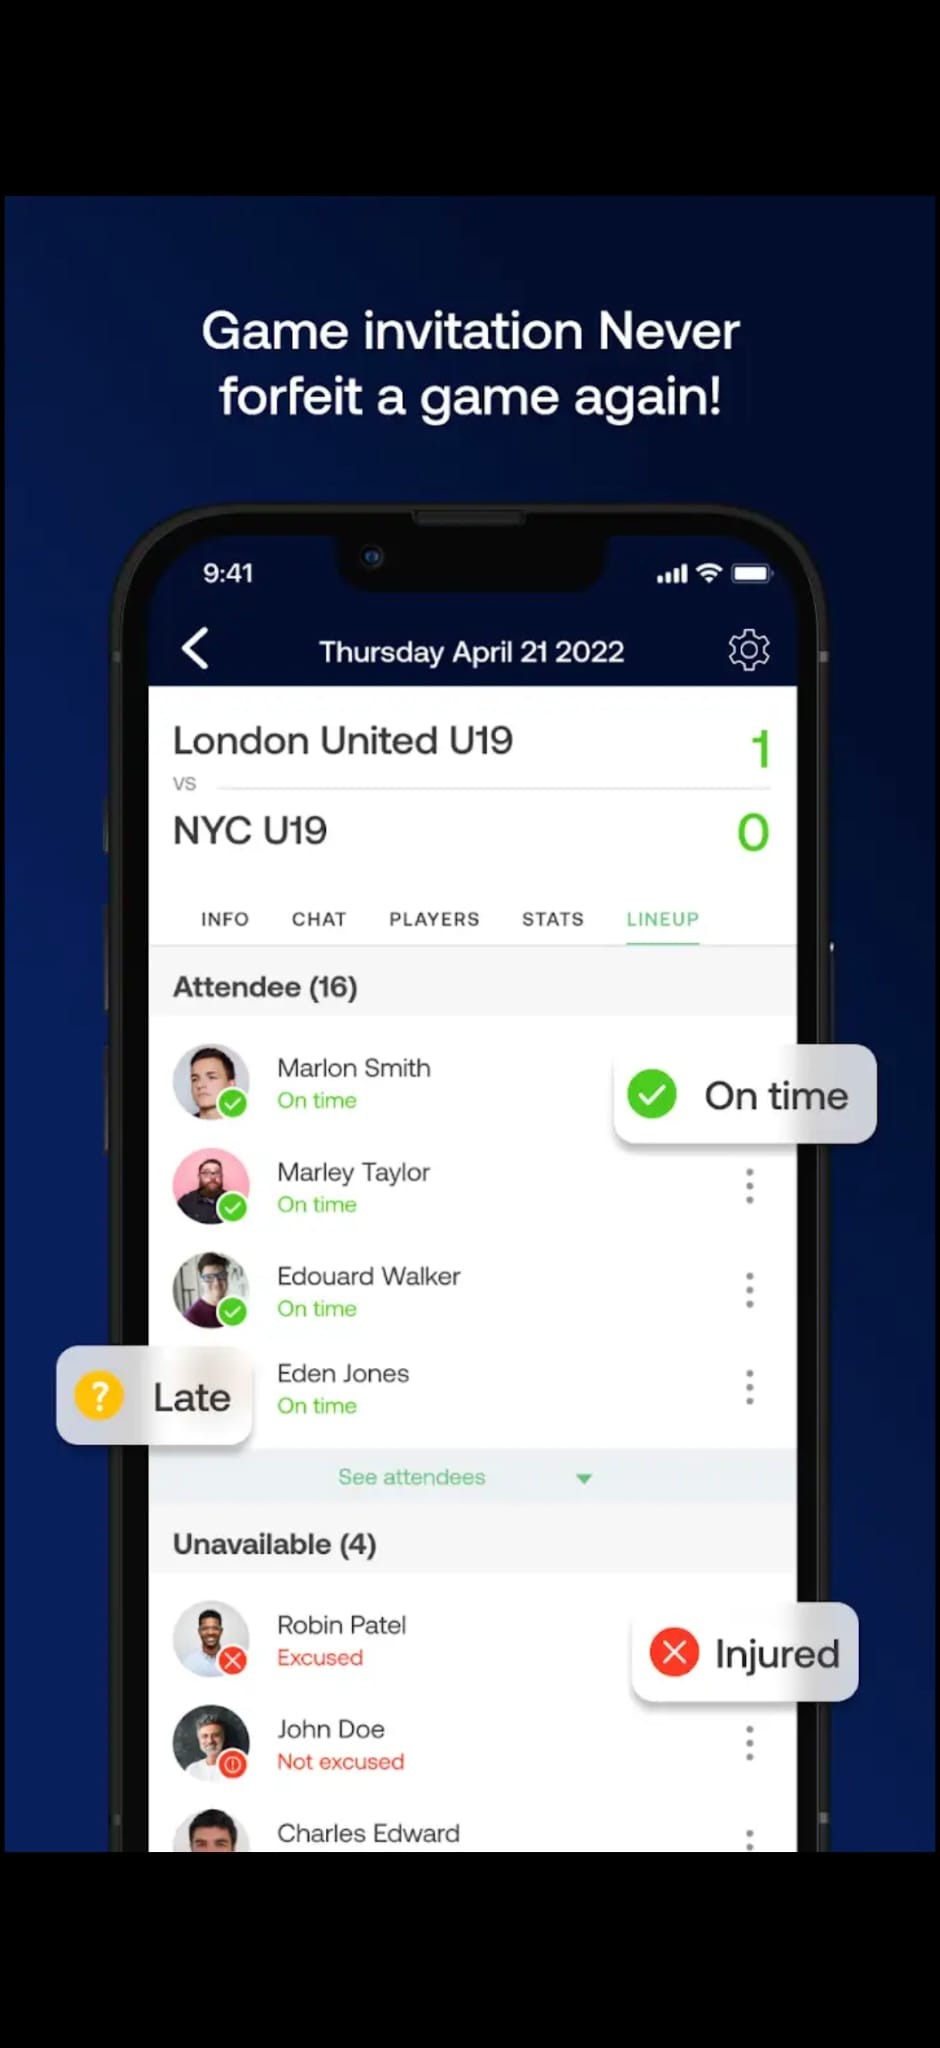
\includegraphics[width=.7\linewidth, height=1.1\linewidth]{imagenes/sportEasy.jpeg}
                \caption{SportEasy \protect\cite{SportEasy}}
                \label{fig:sporteasy_interface}            
            \end{subfigure}\hfill
            \begin{subfigure}{.48\textwidth}
                \centering
                \includegraphics[width=.7\linewidth, height=1.1\linewidth]{imagenes/Playoff.jpeg}
                \caption{Playoff \protect\cite{Playoff}}
                \label{fig:playoff_interface}            
            \end{subfigure}
            
            \vspace{0.5cm} % Espacio vertical entre la primera y segunda fila
            
            % Segunda fila: 2 figuras
            \begin{subfigure}{.48\textwidth}
                \centering
                \includegraphics[width=.7\linewidth, height=1.1\linewidth]{imagenes/TeamSnap.jpeg}
                \caption{TeamSnap \protect\cite{TeamSnap}}
                \label{fig:teamsnap_interface}            
            \end{subfigure}\hfill
            \begin{subfigure}{.48\textwidth}
                \centering
                \includegraphics[width=.7\linewidth, height=1.1\linewidth]{imagenes/Sprongo.jpeg}
                \caption{Sprongo \protect\cite{Sprongo}}
                \label{fig:sprongo_interface}            
            \end{subfigure}
            
            \vspace{0.5cm} % Espacio vertical entre la segunda y tercera fila
            
            % Tercera fila: 1 figura centrada
            \begin{subfigure}{\textwidth}
                \centering
                \includegraphics[width=.33\linewidth, height=0.52\linewidth]{imagenes/Onesporter.jpeg}
                \caption{Onesporter \protect\cite{Onesporter}}
                \label{fig:onesporter_interface}            
            \end{subfigure}
            
            \caption{Interfaces de las soluciones de software analizadas en el estudio competitivo.}
            \label{fig:analisis_competitivo_interfaces}
        \end{figure}

    \section{Objetivos}
    Dado el contexto analizado y las oportunidades de mejora detectadas, estos son los objetivos específicos del proyecto:

    \begin{itemize}
        \item \textbf{Diseñar e implementar la base de datos:} Modelar una estructura relacional en MySQL para almacenar de forma segura y organizada la información de los deportistas, entrenadores, eventos y el histórico de asistencia por temporadas.
        
        \item \textbf{Desarrollo del servicio backend:} Construir una API REST en Node.js con Express estructurada en controladores y rutas independientes para gestionar de manera eficiente todas las peticiones del sistema.
        
        \item \textbf{Garantizar la seguridad mediante roles:} Implementar un sistema de autenticación basado en JSON Web Tokens (JWT) que restrinja el acceso a las rutas del backend según el perfil del usuario (Administrador, Entrenador o Padre).
        
        \item \textbf{Crear la interfaz de usuario móvil:} Desarrollar una aplicación multiplataforma utilizando React Native y Context API que sea ligera, intuitiva y fácil de usar en las condiciones extremas a pie de pista.
        
        \item \textbf{Integrar analítica estadística visual:} Incorporar la librería \textit{react-native-chart-kit} para transformar los registros numéricos de asistencia y entrenamientos en gráficos estadísticos claros que muestren la progresión de los atletas.
        
        \item \textbf{Centralizar la gestión multimedia técnica:} Diseñar un repositorio indexado dentro de la aplicación para que los entrenadores puedan subir fotos y vídeos de los descensos, vinculándolos directamente al perfil de cada deportista para su corrección técnica.
    \end{itemize}

    Con todo ello, la gestión diaria del club de esquí y el seguimiento de los deportistas de base será no solo más eficiente y automatizado, sino también transparente y accesible para los entrenadores y las familias.
\chapter{Tecnologías y Herramientas Utilizadas}
\label{cap:tecnologias_utilizadas}

El desarrollo de la plataforma \textit{SkiClubManager} se ha basado en una arquitectura desacoplada compuesta por un servicio de \textit{backend} centralizado y una aplicación móvil nativa como \textit{frontend}. La selección de la pila tecnológica (\textit{stack}) responde a criterios estrictos de rendimiento, mantenibilidad y la necesidad de ofrecer una experiencia de usuario fluida en entornos de alta montaña. A continuación, se justifican técnicamente las herramientas y entornos seleccionados.

\subsubsection{Infraestructura Backend y API REST}
Para dar soporte a la aplicación móvil y centralizar la lógica de negocio, se ha diseñado un servicio backend basado en una arquitectura cliente-servidor mediante el desarrollo de una API REST.

\subsubsection{Node.js}
Node.js es un entorno de ejecución para JavaScript construido con el motor V8 de Google \cite{NodeJS}. Su elección como núcleo del \textit{backend} se justifica por las siguientes características:
\begin{itemize}
    \item \textbf{Modelo de E/S sin bloqueo y orientado a eventos:} Utiliza un único hilo de ejecución asistido por un bucle de eventos (\textit{Event Loop}). Esto permite gestionar múltiples conexiones concurrentes de forma asíncrona sin bloquear el servidor, una cualidad crítica cuando entrenadores y familias interactúan con la aplicación simultáneamente.
    \item \textbf{Unificación del lenguaje:} El uso de JavaScript tanto en el servidor como en el cliente (\textit{frontend}) optimiza los tiempos de desarrollo, reduce la curva de aprendizaje y simplifica el mantenimiento del código fuente global.
\end{itemize}

\subsubsection{Express}
Express es un \textit{framework} minimalista y flexible creado para Node.js \cite{ExpressJS}, seleccionado para estructurar la API REST debido a su solvencia en el manejo de peticiones HTTP:
\begin{itemize}
    \item \textbf{Arquitectura basada en Middleware:} Organiza el flujo de las peticiones mediante funciones interconectadas. Esto permite auditar, transformar o validar los datos de entrada antes de que alcancen la lógica de negocio final.
    \item \textbf{Enrutamiento modular:} Permite desglosar las rutas de la API en controladores independientes, garantizando un código limpio, escalable y alineado con los principios de diseño de software modular.
\end{itemize}

\subsubsection{Motor de Persistencia: MySQL}
Como sistema de gestión de bases de datos se ha seleccionado MySQL \cite{MySQL}, un motor relacional de código abierto que garantiza el almacenamiento seguro y consistente de la información del club. Su elección se fundamenta en su capacidad para gestionar restricciones de integridad referencial mediante claves foráneas, asegurando que las asistencias, transportes y expedientes queden vinculados de forma unívoca y protegida a las fichas de los deportistas menores de edad.

\subsubsection{Desarrollo Frontend Móvil}
La capa de interacción con el usuario final requiere un entorno capaz de ofrecer portabilidad sin penalizar el rendimiento en dispositivos móviles.

\subsubsection{React Native}
React Native es un \textit{framework} de código abierto desarrollado por Meta \cite{ReactNative} que permite compilar aplicaciones móviles nativas para iOS y Android a partir de una única base de código en JavaScript y React. Los motivos técnicos de su elección incluyen:
\begin{itemize}
    \item \textbf{Renderizado Nativo:} A diferencia de las soluciones híbridas basadas en vistas web, React Native invoca directamente los componentes nativos del sistema operativo, garantizando una interfaz fluida y una respuesta inmediata a las interacciones del usuario.
    \item \textbf{Eficiencia en Entornos de Nieve:} La ligereza de la aplicación y la velocidad de respuesta de sus componentes son críticas para el cuerpo técnico en las pistas de esquí, donde las bajas temperaturas exteriores exigen flujos de trabajo rápidos y pantallas de carga mínimas.
\end{itemize}

\subsubsection{Gestión de Estado: Context API}
Para la propagación del estado global de la aplicación se ha utilizado la herramienta nativa \textit{Context API} de React. Este mecanismo permite inyectar los datos de la sesión activa, el rol del usuario autenticado (Entrenador o Padre) y los filtros temporales a lo largo de todo el árbol de componentes sin necesidad de recurrir a librerías externas complejas, facilitando el renderizado condicional inmediato de la interfaz.

\subsubsection{Autenticación: JSON Web Tokens (JWT)}
La seguridad y el aislamiento de los datos sensibles se gestionan mediante el estándar abierto RFC 7519, conocido como JSON Web Tokens \cite{RFC7519_JWT}. Tras un inicio de sesión exitoso, el servidor genera un token firmado criptográficamente que la aplicación móvil almacena de forma segura. Este token se adjunta en las cabeceras de cada petición HTTP, garantizando la autenticidad del emisor y permitiendo la validación de roles en cada \textit{endpoint} de la API REST.

\subsubsection{Visualización Analítica: React Native Chart Kit}
Para la representación gráfica del rendimiento de los corredores y los balances de asistencia en los perfiles familiares, se ha implementado la librería complementaria \textit{react-native-chart-kit} \cite{ReactNativeChartKit}. Esta herramienta se acopla directamente sobre el flujo de datos del estado global, transformando registros relacionales planos de asistencia en métricas visuales comprensibles y optimizadas para su correcta renderización en dispositivos móviles.

\subsubsection{Diseño de Interfaces: Figma}
Como entorno de prototipado industrial se ha empleado Figma. Esta herramienta basada en la nube ha permitido modelar la arquitectura de la información y evolucionar los esquemas desde \textit{wireframes} de baja fidelidad hasta los \textit{mockups} de alta fidelidad que sirven como plano técnico exacto para la maquetación visual de la aplicación móvil.
\chapter{Análisis y Diseño}

En este capítulo se desglosan las decisiones arquitectónicas que articulan el proyecto, estructuradas en tres ejes principales: el diseño del almacén de datos, la lógica de interconexión entre las capas del sistema (frontend y backend) y el modelado de la interfaz de usuario. A través de este análisis se demuestra cómo cada componente ha sido planificado estratégicamente para ofrecer un desarrollo escalable en \textit{Node.js} y \textit{React Native}, garantizando una experiencia fluida para administrador, entrenadores y padres

\section{Planificación del proyecto}
    \subsubsection{Diagrama de Gantt}
    El diagrama de \textit{Gantt} a continuación muestra la planificación detallada de todas las actividades realizadas durante el desarrollo del proyecto. Este diagrama refleja la secuencia, duración y solapamiento de las diferentes tareas, ofreciendo una visión global de la gestión del tiempo y recursos a lo largo de todo el proceso.
    \begin{figure}[htbp]
        \centering
        \scriptsize
        \resizebox{\textwidth}{!}{%
            \begin{ganttchart}[
                hgrid,
                vgrid={*{6}{draw=none}, dotted},
                title/.append style={fill=blue!10},
                title label font=\tiny,
                title height=1,
                bar/.append style={fill=gray!30},
                bar height=.4,
                y unit chart=0.5cm,
                x unit=0.12cm,
                time slot format=isodate,
                milestone left shift=-1,
                milestone right shift=2
            ]{2026-02-01}{2026-06-05}
            
                \gantttitlecalendar{month=name} \\
                
                \ganttgroup{Análisis y Aprendizaje}{2026-02-01}{2026-02-14} \\
                    \ganttbar{Definición de alcance y requisitos}{2026-02-01}{2026-02-07} \\
                    \ganttbar{Investigación de tecnologías}{2026-02-08}{2026-02-14} \\
        
                \ganttgroup{Diseño de la Aplicación}{2026-02-15}{2026-02-28} \\
                    \ganttbar{Diseño del modelo entidad-relación}{2026-02-15}{2026-02-21} \\
                    \ganttbar{Bocetos de interfaz móvil}{2026-02-22}{2026-02-28} \\

                \ganttgroup{Desarrollo del Back-End}{2026-03-01}{2026-04-11} \\
                    \ganttbar{Configuración del entorno y MySQL}{2026-03-01}{2026-03-10} \\
                    \ganttbar{Implementación de controladores y lógica}{2026-03-11}{2026-03-25} \\
                    \ganttbar{Desarrollo de endpoints y JWT}{2026-03-26}{2026-04-11} \\
                    
                \ganttgroup{Desarrollo del Front-End}{2026-04-12}{2026-05-16} \\
                    \ganttbar{Estructura de vistas en React Native}{2026-04-12}{2026-04-25} \\
                    \ganttbar{Integración de API de contexto y lógica}{2026-04-26}{2026-05-05} \\
                    \ganttbar{Conexión con API y gráficos}{2026-05-06}{2026-05-16} \\
                
                \ganttgroup{Despliegue y Pruebas}{2026-05-17}{2026-05-31} \\
                    \ganttbar{Pruebas unitarias y del sistema}{2026-05-17}{2026-05-24} \\
                    \ganttbar{Ajustes finales y despliegue}{2026-05-25}{2026-05-31} \\
                
                \ganttgroup{Documentación Transversal}{2026-02-01}{2026-06-05} \\
                    \ganttbar{Redacción de la memoria del TFG}{2026-02-01}{2026-05-20} \\
                    \ganttbar{Revisiones finales y correcciones}{2026-05-21}{2026-06-05} \\
                    
            \end{ganttchart}
        }
        \caption{Diagrama de Gantt detallado con la planificación y fases de desarrollo}
        \label{fig:gantt_diagram_detailed}
    \end{figure}

    \newpage
    \subsubsection{Cronograma}
        \begin{table}[htbp]
            \centering
            \begin{tabular}{|l|c|}
            \hline
            \textbf{Fase} & \textbf{Duración} \\ \hline
            Análisis y aprendizaje & 2 semanas (14 días) \\ \hline
            Diseño de la aplicación & 2 semanas (14 días) \\ \hline
            Desarrollo del Backend & 6 semanas (42 días) \\ \hline
            Desarrollo del Frontend & 5 semanas (35 días) \\ \hline
            Despliegue y Pruebas & 2 semanas (15 días) \\ \hline
            Documentación transversal & 18 semanas (125 días) \\ \hline
            \end{tabular}
            \caption{Resumen de las fases del proyecto y su duración real}
            \label{tab:duracion_fases_real}
        \end{table}

    Como se puede observar en la Tabla~\ref{tab:duracion_fases_real}, el proyecto se compone de seis fases principales distribuidas a lo largo del segundo cuatrimestre. Es imperativo destacar que la fase de \textit{Documentación} posee un carácter transversal, desarrollándose de forma simultánea y paralela junto con las fases de diseño, desarrollo e implementación del sistema \textit{Full-Stack}.
    
    \section{Recursos y costes}
    \label{sec:recursos_costes}

    Esta sección recoge el coste real de los servicios externos aplicados en el desarrollo del TFG y una estimación de referencia del esfuerzo profesional equivalente para la replicación del sistema.

    \subsubsection{Recursos materiales y software}

    El \textit{stack} tecnológico seleccionado para \textit{SkiClubManager} ha sido elegido bajo la premisa de priorizar herramientas de código abierto, reduciendo el coste directo de licencias a 0 €. El desarrollo principal se realizó en un ordenador de sobremesa adquirido por un importe de 1\,450 €. Siguiendo las directrices estándar de ingeniería, no se imputa el precio íntegro del equipo, sino la parte proporcional al tiempo dedicado al TFG: considerando una vida útil estimada de cuatro años (48 meses), el coste mensual es de $1\,450 / 48 \approx 30$ €/mes. Aplicado a los cinco meses de duración del desarrollo (febrero--junio 2026), el importe de amortización resultante es de 150 €.

    En la tabla \ref{tab:recursos_materiales} se desglosan los recursos materiales y servicios externos utilizados durante la ejecución del proyecto.

    \begin{table}[htbp]
    \centering
    \scriptsize
    \renewcommand{\arraystretch}{1.1}
    \begin{tabularx}{\textwidth}{|l|X|c|l|}
    \hline
    \rowcolor[HTML]{EFEFEF} 
    \textbf{Recurso} & \textbf{Uso en SkiClubManager} & \textbf{Coste} & \textbf{Observaciones} \\ \hline
    Ordenador & IDE, emuladores Android/iOS, compilación & 150 € & Amortización de equipo propio \\ \hline
    Stack open source & Backend (Node.js), Frontend (React Native), BD (MySQL) & 0 € & Licencia libre \\ \hline
    \textbf{Total materiales} & & \textbf{150 €} & \\ \hline
    \end{tabularx}
    \caption{Recursos materiales y servicios externos.}
    \label{tab:recursos_materiales}
    \end{table}

    \subsubsection{Estimación de esfuerzo y coste laboral}
    Como tarifa de referencia para el cálculo del coste laboral, se ha tomado como base el XVII Convenio Colectivo Estatal de Empresas de Consultoría y Tecnologías de la Información, publicado en el BOE núm. 178, de 27 de julio de 2023 \cite{boe_convenio_consultoria}. Para un perfil de desarrollador \textit{full-stack} júnior, se adopta la categoría de Programador o Técnico de Sistemas (Área 3, Grupo E, Nivel E2).

    El salario mínimo garantizado por convenio para esta categoría, actualizado al año de ejercicio actual, se sitúa en torno a los 21\,500 € brutos anuales. A este importe se le añade un 32\% en concepto de costes sociales obligatorios a cargo de la empresa (Seguridad Social, contingencias comunes, formación y desempleo), elevando el coste total anual para la organización a 28\,380 €. 

    Considerando la jornada máxima anual establecida por dicho convenio de 1\,800 horas laborables, el coste horario real de ingeniería se calcula mediante la fórmula:
    
    $$\mathrm{Coste\ por\ hora} = \frac{28\,380\ \mathrm{EUR}}{1\,800\ \mathrm{h}} \approx 15,76\ \mathrm{EUR/h}$$    
    
    Para dotar al presupuesto de un margen de contingencia profesional y alinearlo con los precios medios de mercado para servicios de consultoría júnior, se establece una tarifa de **18 \euro/h**. Por tanto, el coste laboral de referencia para las 580 horas de dedicación queda establecido en $580 \times 18 = 10\,440$ €.

    \subsubsection{Presupuesto total}

    El presupuesto global estimado para la replicación del proyecto integra tanto los costes tangibles directos como la valoración del esfuerzo de ingeniería. La tabla \ref{tab:presupuesto_total} consolida el presupuesto final de la aplicación.

    \begin{table}[htbp]
    \centering
    \scriptsize
    \renewcommand{\arraystretch}{1.1}
    \begin{tabularx}{\textwidth}{|l|c|X|}
    \hline
    \rowcolor[HTML]{EFEFEF} 
    \textbf{Concepto} & \textbf{Importe} & \textbf{Notas} \\ \hline
    Ordenador (amortización) & 150 € & $1\,450 / 48 \times 5 \approx 150$ € \\ \hline
    Software & 0 € & Entorno open source sin costes de licencia \\ \hline
    Mano de obra (Convenio BOE) & 10\,440 € & 580 h $\times$ 18 €/h \\ \hline
    \textbf{Total estimado de replicación} & \textbf{10\,615 €} & \\ \hline
    \end{tabularx}
    \caption{Presupuesto total estimado del proyecto.}
    \label{tab:presupuesto_total}
    \end{table}

    \section{Análisis}
    \subsubsection{Definición de Requisitos y Flujos de Interacción}
        \subsubsection{Requisitos Funcionales y No Funcionales}
        En este apartado se detallan los requisitos que debe cumplir la aplicación para garantizar
        su correcto funcionamiento. Se clasifican en dos categorías: los requisitos funcionales, que
        describen las funcionalidades y características específicas que debe proporcionar el sistema,
        y los requisitos no funcionales, que establecen las condiciones y restricciones de calidad,
        usabilidad, rendimiento y seguridad que debe cumplir la aplicación.

        \subsection{Requisitos Funcionales}

        A continuación, se describen de manera detallada los requisitos funcionales del sistema, organizados por módulos lógicos. Estos especifican las acciones, comportamientos y operaciones que la aplicación informática debe ejecutar para satisfacer las necesidades de gestión del club de esquí alpino.

        \subsubsection*{RF1: Gestión de Usuarios y Roles}
        \begin{itemize}
            \item \textbf{RF1.1: Registro de cuentas de familiares.} La aplicación móvil debe permitir a los nuevos padres registrarse de forma autónoma en el sistema introduciendo sus datos personales, quedando su cuenta en estado pendiente de aprobación.
            \item \textbf{RF1.2: Control y validación de accesos por el administrador.} El sistema debe permitir al administrador, desde su panel de gestión centralizado, supervisar y validar las solicitudes de registro de los nuevos familiares, habilitando sus credenciales en la base de datos de forma segura.
            \item \textbf{RF1.3: Alta centralizada de entrenadores.} El sistema debe permitir únicamente al administrador dar de alta las cuentas del personal técnico y entrenadores en la base de datos, asignándoles una contraseña temporal por defecto.
            \item \textbf{RF1.4: Alta y vinculación de deportistas.} La interfaz móvil con rol de padre debe permitir registrar las fichas de los deportistas (hijos) introduciendo sus datos técnicos e integrándolos automáticamente bajo su tutoría mediante claves foráneas en MySQL.
            \item \textbf{RF1.5: Inicio de sesión y distribución de roles.} La aplicación debe permitir a los usuarios validados iniciar sesión de forma segura. El backend en Node.js emitirá un token JWT conteniendo el rol (Administrador, Entrenador o Padre) para configurar la interfaz en React Native.
            \item \textbf{RF1.6: Persistencia segura de sesión.} El frontend debe almacenar el token JWT de forma persistente en el dispositivo para mantener la sesión activa sin requerir credenciales en cada apertura del sistema.
            \item \textbf{RF1.7: Modificación de contraseña temporal.} El sistema debe permitir a cualquier usuario autentificado editar sus datos de contacto y forzar al entrenador a sustituir la contraseña asignada por defecto por una clave privada y segura.
            \item \textbf{RF1.8: Recuperación de credenciales.} La plataforma debe incorporar un mecanismo de recuperación de contraseña para que cualquier usuario, en caso de olvido, pueda restablecer su acceso mediante un código de validación por correo electrónico.
            \item \textbf{RF1.9: Modificación y actualización de fichas de deportistas.} La interfaz móvil con rol de padre debe permitir la edición posterior de los datos técnicos y de contacto de emergencia de los deportistas asociados a su cuenta.
        \end{itemize}

        \subsubsection*{RF2: Gestión de Entrenamientos}
        \begin{itemize}
            \item \textbf{RF2.1: Programación de eventos.} El usuario con rol de entrenador debe poder crear y calendarizar entrenamientos técnicos, competiciones o sesiones de preparación física, detallando fecha, hora y localización.
            \item \textbf{RF2.2: Inscripción obligatoria por los padres.} La aplicación debe permitir a los padres apuntar o desapuntar a sus hijos de los eventos programados de forma directa, gestionando de manera autónoma la asistencia del deportista.
            \item \textbf{RF2.3: Consulta de asistencia en tiempo real.} El sistema debe ofrecer al entrenador un listado dinámico con los atletas confirmados para cada sesión, permitiéndole conocer de antemano el volumen de alumnos en pista.
            \item \textbf{RF2.4: Gestión de eventos programados.} El sistema debe permitir al entrenador modificar o cancelar entrenamientos debido a contingencias climáticas o logísticas de la estación de esquí, notificando el cambio a los padres.
            \item \textbf{RF2.5: Buscador avanzado de entrenamientos.} La interfaz en React Native debe incorporar un campo de búsqueda que permita a los usuarios filtrar el listado de sesiones planificadas mediante la introducción de texto libre para entrenamientos específicos o mediante la selección de un día concreto.                
        \end{itemize}

        \subsubsection*{RF3: Gestión Multimedia}
        \begin{itemize}
            \item \textbf{RF3.1: Almacenamiento de fotografías.} La aplicación móvil debe permitir al usuario con rol de entrenador o administrador cargar imágenes en el servidor, ya sea capturándolas con la cámara del dispositivo o seleccionándolas desde su galería local.
            \item \textbf{RF3.2: Vinculación por categoría o alcance general.} El sistema debe indexar cada fotografía asociándola a una categoría deportiva específica del club o asignándole un identificador de carácter general, almacenando la ruta del archivo correspondiente en el motor de persistencia.
            \item \textbf{RF3.3: Buscador cronológico en galería.} La interfaz en React Native debe incorporar un módulo de búsqueda dentro de la galería que permita filtrar los registros fotográficos mediante consultas por año o mes.
            \item \textbf{RF3.4: Visualización restringida para padres.} El sistema debe garantizar que los usuarios con rol de padre puedan visualizar únicamente las fotografías de carácter general y las publicaciones pertenecientes a la categoría deportiva de sus hijos.
        \end{itemize}

        \subsubsection*{RF4: Gestión de Transporte del Club}
        \begin{itemize}
            \item \textbf{RF4.1: Configuración de capacidad de transporte.} El sistema debe permitir al entrenador vincular un servicio de transporte a cualquier entrenamiento programado, el límite máximo de plazas disponibles en los vehículos del club.
            \item \textbf{RF4.2: Reserva de plazas por los padres.} La aplicación móvil debe ofrecer a los padres la posibilidad de solicitar una plaza de transporte para sus hijos de manera simultánea al proceso de confirmación de asistencia al entrenamiento.
            \item \textbf{RF4.3: Control de aforo en tiempo real.} El backend en Node.js debe verificar de forma activa el número de asientos ocupados en MySQL, denegando nuevas solicitudes automáticamente e informando al usuario en React Native una vez que se alcance el límite de capacidad.
            \item \textbf{RF4.4: Listado logístico de transporte.} El sistema debe proporcionar al entrenador una vista clara y actualizada con la relación de deportistas que han reservado plaza para cada trayecto, facilitando la organización del viaje hacia la estación de esquí.
        \end{itemize}

        \subsubsection*{RF5: Gestión de Asistencias}
        \begin{itemize}
            \item \textbf{RF5.1: Filtrado por tipología de sesión.} La aplicación móvil debe permitir clasificar el historial de asistencias del deportista en función del entorno del entrenamiento, discriminando entre sesiones técnicas en pista y sesiones de preparación física.
            \item \textbf{RF5.2: Selección de deportista vinculado.} El sistema debe proporcionar un selector interactivo en la interfaz del padre que le permita alternar de forma dinámica la visualización de los datos entre los distintos hijos que tenga registrados bajo su tutela.
            \item \textbf{RF5.3: Filtrado cronológico por temporada y mes.} La plataforma debe resolver consultas relacionales que agrupen y muestren de forma integrada todo el registro de asistencias pertenecientes a una temporada completa del club de esquí o acotadas a mensualidades específicas.
            \item \textbf{RF5.4: Renderizado estadístico y gráfico.} El frontend en React Native debe capturar los datos filtrados provenientes de la API y transformarlos de manera automatizada en diagramas y gráficos evolutivos mediante el uso de la librería \textit{react-native-chart-kit}.
            \item \textbf{RF5.5: Restricción de vista para el entrenador.} La aplicación debe limitar la visualización del rol de entrenador de forma estricta a los registros de asistencia globales e individuales de los deportistas que pertenecen exclusivamente a su categoría asignada.
            \item \textbf{RF5.6: Panel de control global para el administrador.} El sistema debe permitir al administrador consultar el histórico de asistencia de la totalidad de los atletas del club, incorporando un selector dinámico para filtrar los resultados por categorías deportivas.
        \end{itemize}  

        \subsection{Requisitos No Funcionales}

        Los requisitos no funcionales definen los atributos de calidad, restricciones técnicas y criterios de rendimiento que debe cumplir el sistema informático. Estos garantizan que la solución de software no solo ejecute las tareas solicitadas, sino que lo haga de forma segura, eficiente, robusta y con una experiencia de usuario óptima.

        \subsubsection*{RNF1: Seguridad y Privacidad}
        \begin{itemize}
            \item \textbf{RNF1.1: Cifrado de credenciales.} Toda contraseña de usuario almacenada en la base de datos MySQL debe ser cifrada de extremo a extremo mediante el uso del algoritmo de hash robusto \textit{bcrypt}, aplicando una función de salado (\textit{salting}) para prevenir ataques de diccionario.
            \item \textbf{RNF1.2: Mecanismo de autenticación sin estado.} El control de sesiones e intercambio de información confidencial entre la aplicación móvil y la API REST debe gestionarse mediante tokens web de JSON (\textit{JSON Web Tokens}, JWT). Estos tokens viajarán firmados digitalmente para evitar su manipulación y tendrán un tiempo de expiración acotado.
            \item \textbf{RNF1.3: Control de accesos basado en roles (RBAC).} El backend en Node.js debe implementar capas de middleware interconectadas encargadas de interceptar cada petición HTTP, validando la firma del token JWT y verificando de forma estricta que el rol del usuario (Administrador, Entrenador o Padre) posea los privilegios específicos para consumir dicho recurso.
            \item \textbf{RNF1.4: Protección de datos sensibles.} Al tratar con información de menores de edad (deportistas), el sistema debe restringir el acceso a datos sensibles de contacto, exponiéndolos exclusivamente a los tutores legales vinculados y al administrador del club.
        \end{itemize}

        \subsubsection*{RNF2: Rendimiento y Escalabilidad}
        \begin{itemize}
            \item \textbf{RNF2.1: Gestión asíncrona de conexiones concurrentes.} El servicio backend basado en Express debe aprovechar el modelo de E/S sin bloqueo y el bucle de eventos (\textit{Event Loop}) de Node.js para mitigar la degradación del rendimiento en picos de alta concurrencia, como las horas previas al inicio de los entrenamientos.
            \item \textbf{RNF2.2: Optimización de transferencias multimedia.} El sistema de almacenamiento y servicio de imágenes técnicas debe optimizar el peso de los archivos cargados antes de su persistencia en el servidor, minimizando el consumo de ancho de banda en los dispositivos móviles que utilicen redes de datos móviles en las estaciones de esquí.
            \item \textbf{RNF2.3: Tiempos de respuesta de la API.} El backend debe procesar las consultas relacionales ordinarias (como listados de asistencia y consultas de calendario) y devolver una respuesta en formato JSON en un tiempo inferior a los 500 milisegundos en condiciones óptimas de red.
        \end{itemize}

        \subsubsection*{RNF3: Disponibilidad y Fiabilidad}
        \begin{itemize}
            \item \textbf{RNF3.1: Tasa de disponibilidad del servicio.} Al tratarse de una aplicación de gestión deportiva crítica para la planificación diaria del club, el despliegue del servidor API y el motor de persistencia MySQL debe garantizar una disponibilidad continua del 99\% mensual.
            \item \textbf{RNF3.2: Persistencia transaccional de datos.} El motor de base de datos debe operar bajo el motor de almacenamiento InnoDB para asegurar el cumplimiento de las propiedades ACID (Aislamiento, Consistencia, Integridad y Durabilidad), garantizando que las transacciones complejas de asistencias concurrentes se ejecuten por completo o se reviertan de forma segura.
        \end{itemize}

        \subsubsection*{RNF4: Usabilidad y Compatibilidad}
        \begin{itemize}
            \item \textbf{RNF4.1: Diseño de interfaz adaptativa y móvil.} El frontend desarrollado en React Native debe implementar un diseño de interfaz responsivo y coherente, optimizado tanto para dispositivos iOS como Android, garantizando que los elementos visuales y los formularios sean accesibles y legibles en pantallas de distintas dimensiones.
            \item \textbf{RNF4.2: Experiencia de usuario en entornos invernales.} La interfaz gráfica debe priorizar el uso de componentes interactivos de gran tamaño, tipografías contrastadas y selectores ágiles, facilitando la operativa del entrenador en la pista de esquí a bajas temperaturas y bajo condiciones lumínicas extremas.
        \end{itemize}

        \subsection{Descripción de los Implicados}

        En el contexto de la aplicación, los implicados desempeñan diferentes roles que son cruciales para su funcionamiento y evolución. A continuación, se presentan los tipos de implicados y sus respectivas responsabilidades de forma estructurada:

        \begin{table}[htbp]
            \centering
            \begin{tabularx}{\textwidth}{|l|>{\raggedright\arraybackslash}X|c|>{\raggedright\arraybackslash}X|}
            \hline
            \textbf{Nombre} & \textbf{Descripción} & \textbf{Tipo} & \textbf{Rol} \\ \hline
            Administrador & Personal de dirección o administración del club de esquí. & Interno & Supervisar y validar registros, dar de alta al personal técnico y auditar asistencias globales. \\ \hline
            Entrenador & Personal técnico profesional responsable de la parte deportiva. & Interno & Programar entrenamientos, gestionar furgonetas y multimedia. \\ \hline
            Padres / Tutores & Familiares y representantes legales de los atletas menores de edad. & Externo & Consultar calendario, confirmar asistencia y reservar transporte. \\ \hline
            Deportistas & Atletas menores de edad pertenecientes a las categorías del club. & Indirecto & Beneficiarios del sistema. No operan la app por seguridad, pero sus datos centralizan el sistema. \\ \hline
            Desarrollador & Ingeniero de software responsable de la creación técnica del proyecto. & Externo & Diseñar la arquitectura, implementar código, desplegar la base de datos y dar soporte técnico. \\ \hline
            \end{tabularx}
            \caption{Implicados en la Aplicación}
            \label{tab:implicados_aplicacion}
        \end{table}
        \newpage
        \subsubsection{Casos de Uso}
        Los casos de uso describen las interacciones entre los usuarios y el sistema, detallando cómo se comporta la aplicación para satisfacer las necesidades del usuario. Esta sección tiene como objetivo presentar los diferentes escenarios en los que los usuarios pueden interactuar con la aplicación y cómo el sistema responde a esas acciones. Los elementos que forman un caso de uso incluyen:

        \begin{description}
            \item[Nombre del Caso de Uso:] Descripción breve y clara de la funcionalidad que se va a representar.
            \item[Actores:] Usuarios o sistemas externos que interactúan con el sistema en el caso de uso.
            \item[Descripción:] Explicación del flujo principal del caso de uso, destacando los pasos principales.
            \item[Precondiciones:] Condiciones que deben cumplirse antes de que el caso de uso pueda ser ejecutado.
            \item[Flujo Principal:] Secuencia de pasos que describen cómo se lleva a cabo el caso de uso bajo circunstancias normales.
            \item[Flujo Alternativo:] Variaciones o excepciones al flujo principal, describiendo cómo se manejarían otras posibles situaciones.
            \item[Postcondiciones:] Estado final del sistema después de que el caso de uso ha sido ejecutado.
            \item[Requisitos Asociados:] Requisitos funcionales que se cumplen al llevar a cabo este caso de uso.
        \end{description}
        
        A continuación, se introduce el diagrama de paquetes que representa la arquitectura modular del sistema, mostrando la organización y dependencias.

        \begin{figure}[htbp]
        \centering
        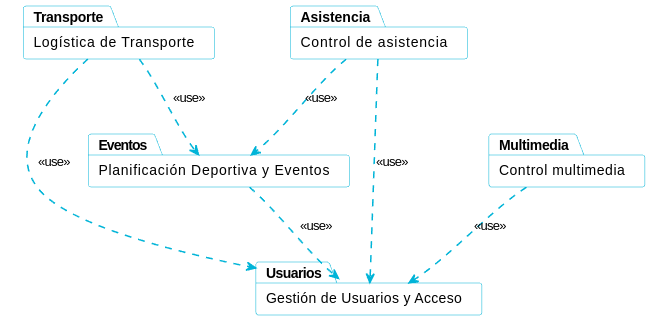
\includegraphics[width=0.6\textwidth]{diagramas/DiagramaPaquetes.drawio.png}
        \caption{Diagrama de paquetes del sistema.}
        \label{fig:diagrama_paquetes}
        \end{figure}
        
        \newpage
        \subsubsection{Módulo de gestión de usuarios y acceso.}
        Este módulo engloba la lógica de control de acceso, registro y seguridad perimetral de la plataforma. 
        \begin{figure}[htbp]
        \centering
        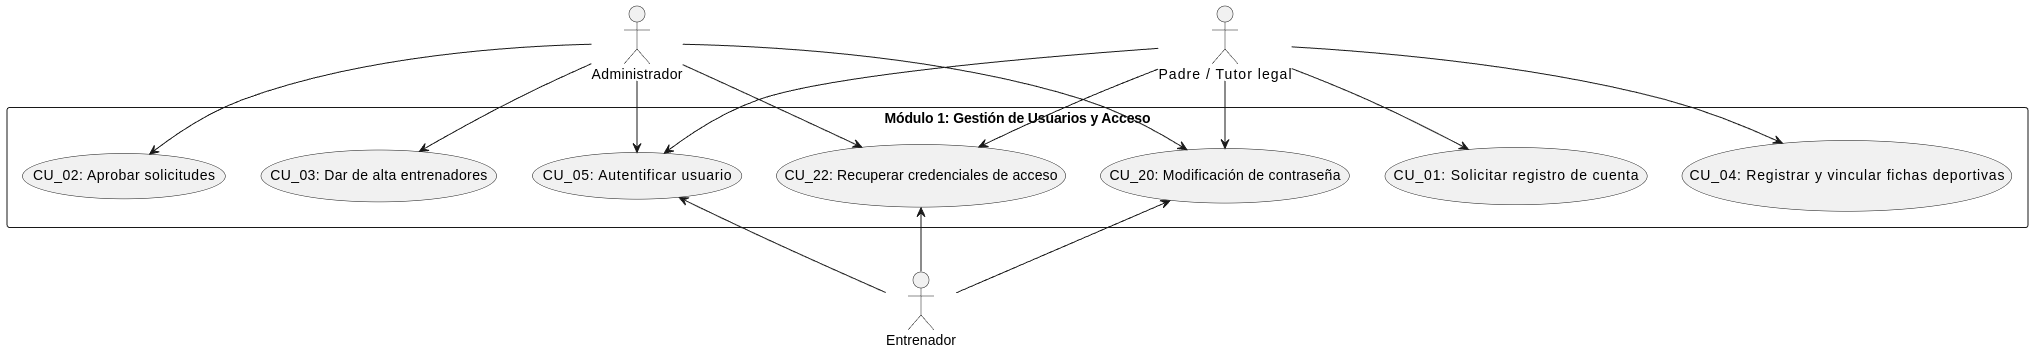
\includegraphics[width=1\textwidth]{diagramas/DiagramaGestionUsuariosYAcceso.drawio.png}
        \caption{Diagrama de gestión de usuarios y acceso.}
        \label{fig:diagrama_gestion_usuarios_acceso}

        \end{figure}
        \begin{table}[htbp]
        \centering
        \footnotesize
        \renewcommand{\arraystretch}{1.0}
        \begin{tabularx}{\textwidth}{|l|X|}
        \hline
        \rowcolor[HTML]{EFEFEF} 
        \textbf{Caso de Uso} & \textbf{Solicitar registro de cuenta (CU\_01)} \\ \hline
        \textbf{Actores} & Padre / Tutor legal \\ \hline
        \textbf{Tipo} & Primario y esencial. \\ \hline
        \textbf{Referencias} & RF1.1 \\ \hline
        \textbf{Precondición} & El usuario no debe de estar registrado en el sistema. \\ \hline
        \textbf{Postcondición} & El usuario está registrado en el sistema. \\ \hline
        \textbf{Propósito} & Permitir a los nuevos usuarios registrarse proporcionando sus datos. \\ \hline
        \textbf{Resumen} & Un usuario desea registrarse para acceder a la aplicación. Introduce los datos requeridos en el formulario de registro y el sistema valida y almacena la información relacionada con el registro. \\ \hline
        \textbf{Curso Normal (Básico)} & 
        \textbf{1.} El usuario accede a la pantalla de registro.\newline
        \textbf{2.} El usuario proporciona los datos necesarios.\newline
        \textbf{3.} El sistema verifica que los datos introducidos sean válidos.\newline
        \textbf{4.} El sistema almacena la petición. \\ \hline
        \textbf{Cursos Alternos} & 
        \textbf{3a:} El correo introducido ya está dado de alta.\newline
        \textbf{3b:} El correo tiene un formato erróneo.\newline
        \textbf{3c:} La contraseña y la confirmación no coinciden. \\ \hline
        \end{tabularx}
        \caption{Ficha caso de uso CU\_01.}
        \label{tab:cu_01}
        \end{table}

        \begin{figure}[htbp]
            \centering
            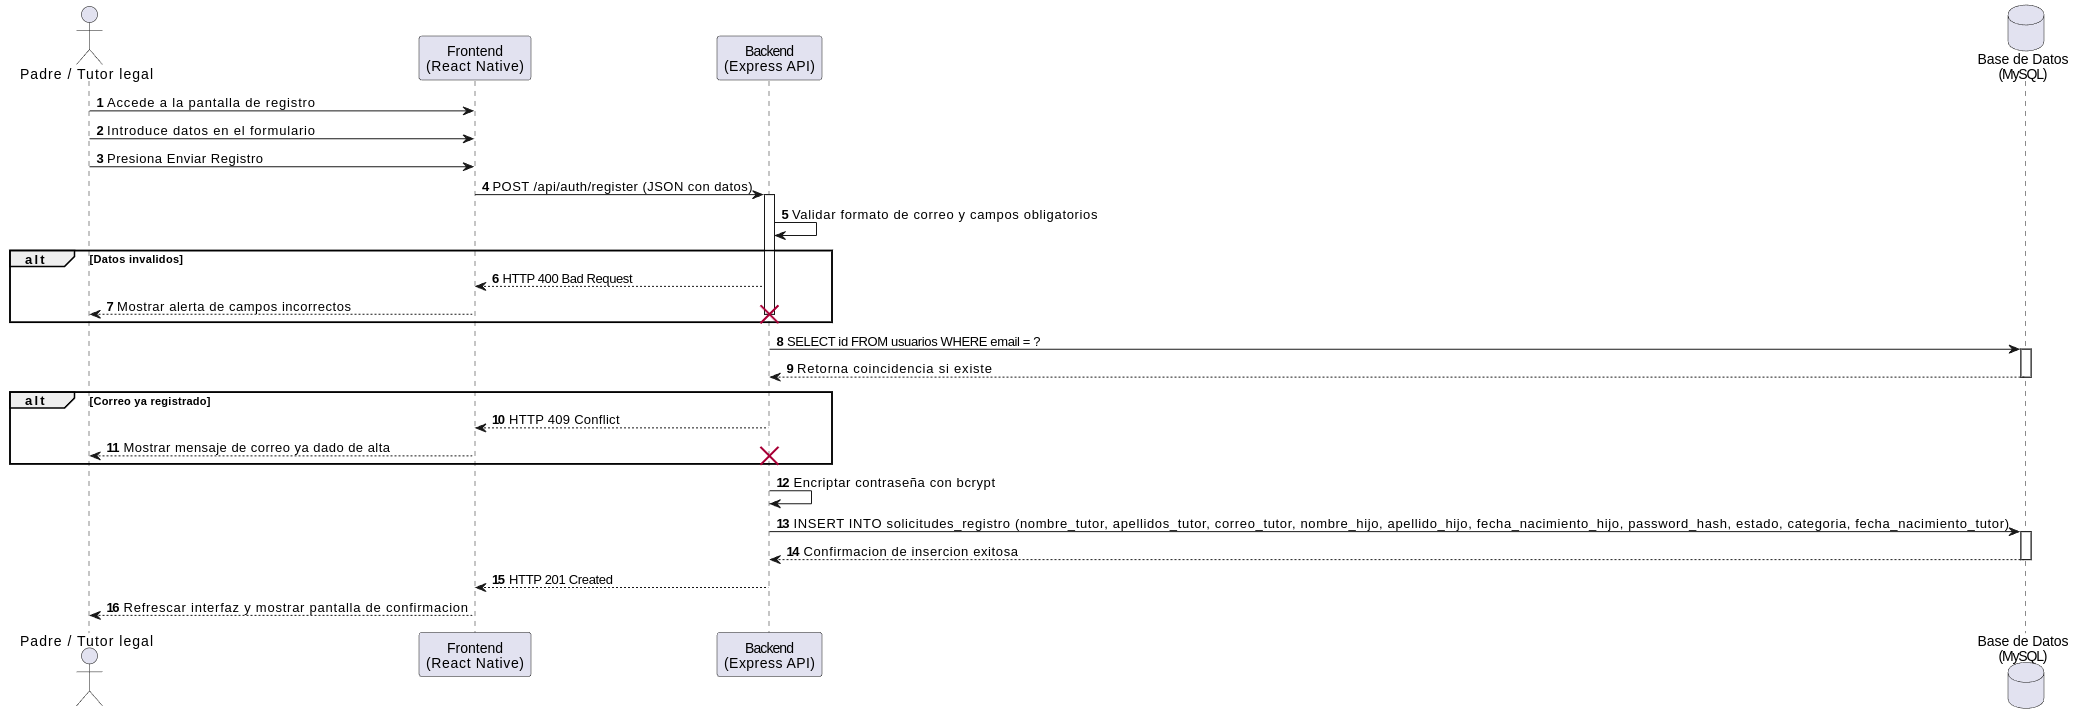
\includegraphics[width=1\textwidth]{diagramas/CU_01.drawio.png}
            \caption{Diagrama de secuencia del CU\_01.}
            \label{fig:seq_cu_01}
        \end{figure}

        \begin{table}[htbp]
        \centering
        \footnotesize
        \renewcommand{\arraystretch}{1.0}
        \begin{tabularx}{\textwidth}{|l|X|}
        \hline
        \rowcolor[HTML]{EFEFEF} 
        \textbf{Caso de Uso} & \textbf{Aprobar solicitudes (CU\_02)} \\ \hline
        \textbf{Actores} & Administrador \\ \hline
        \textbf{Tipo} & Primario y esencial. \\ \hline
        \textbf{Referencias} & RF1.2 \\ \hline
        \textbf{Precondición} & Tiene que haber una solicitud creada por el padre. \\ \hline
        \textbf{Postcondición} & El usuario está creado. \\ \hline
        \textbf{Propósito} & Una vez aprobada la solicitud se crea el usuario. \\ \hline
        \textbf{Resumen} & El administrador gestiona las solicitudes; una vez aceptada, los datos son almacenados en la base de datos. \\ \hline
        \textbf{Curso Normal} & 
        \textbf{1.} El administrador accede a la página de administrar solicitud.\newline
        \textbf{2.} El administrador mira que los datos sean correctos.\newline
        \textbf{3.} El administrador acepta la solicitud.\newline
        \textbf{4.} El sistema almacena la información en la base de datos y activa el usuario. \\ \hline
        \textbf{Cursos Alternos} & 
        \textbf{3a:} Alguno de los datos son incorrectos y el administrador rechaza la solicitud. \\ \hline
        \end{tabularx}
        \caption{Ficha caso de uso CU\_02.}
        \label{tab:cu_02}
        \end{table}

        \begin{figure}[htbp]
            \centering
            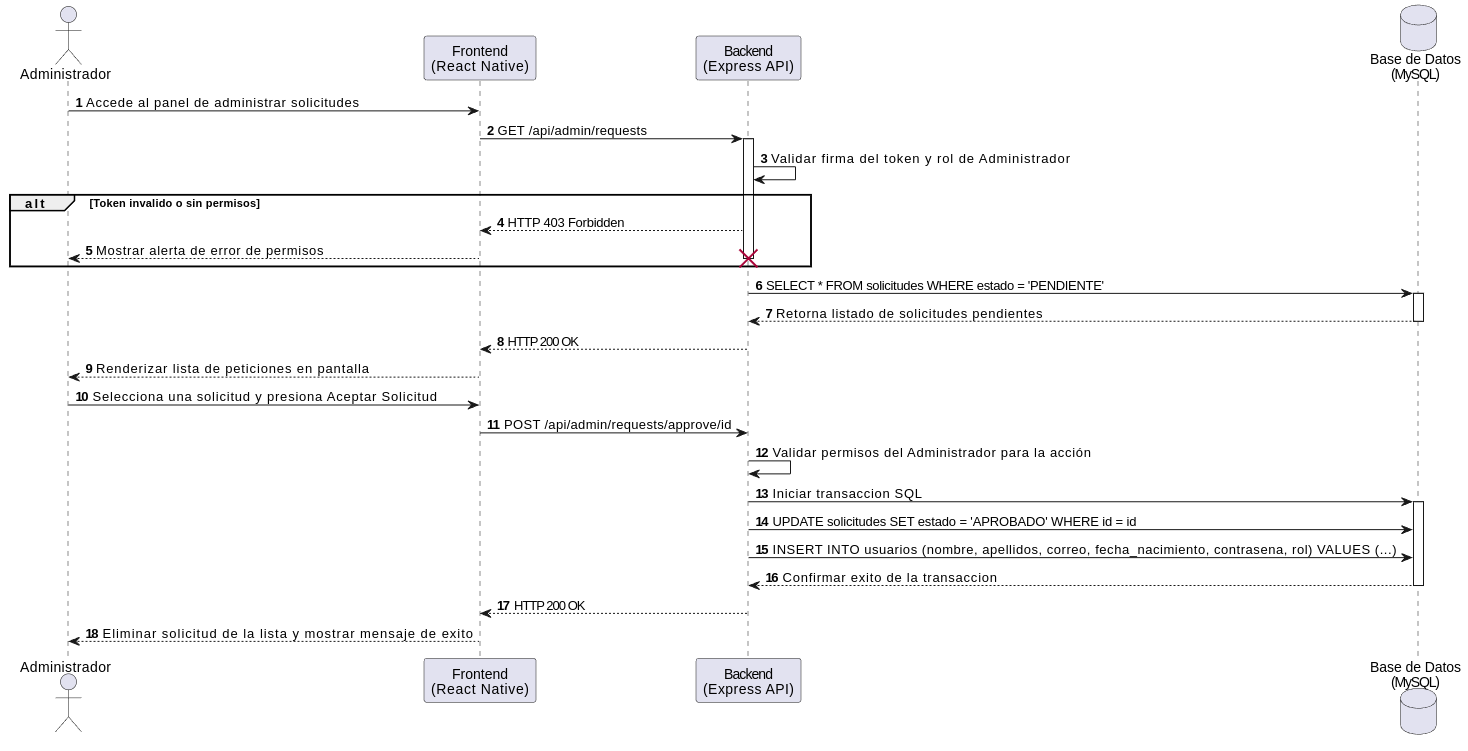
\includegraphics[width=1\textwidth]{diagramas/CU_02.drawio.png}
            \caption{Diagrama de secuencia del CU\_02.}
            \label{fig:seq_cu_02}
        \end{figure}
        
        \newpage
        \begin{table}[htbp]
        \centering
        \footnotesize
        \renewcommand{\arraystretch}{1.0}
        \begin{tabularx}{\textwidth}{|l|X|}
        \hline
        \rowcolor[HTML]{EFEFEF} 
        \textbf{Caso de Uso} & \textbf{Dar de alta entrenadores (CU\_03)} \\ \hline
        \textbf{Actores} & Administrador \\ \hline
        \textbf{Tipo} & Primario y esencial. \\ \hline
        \textbf{Referencias} & RF1.3 \\ \hline
        \textbf{Precondición} & No tiene que existir usuario entrenador. \\ \hline
        \textbf{Postcondición} & El entrenador está creado. \\ \hline
        \textbf{Propósito} & Creación centralizada de los usuarios cuyo rol es entrenador. \\ \hline
        \textbf{Resumen} & El administrador crea al usuario entrenador de manera que esté centralizado. \\ \hline
        \textbf{Curso Normal} & 
        \textbf{1.} El administrador accede a la página de administrar entrenadores.\newline
        \textbf{2.} El administrador rellena los datos correspondientes.\newline
        \textbf{3.} El sistema verifica que los datos son correctos.\newline
        \textbf{4.} El sistema almacena y crea el usuario entrenador. \\ \hline
        \textbf{Cursos Alternos} & 
        \textbf{3a:} El correo introducido ya está dado de alta.\newline
        \textbf{3b:} El correo tiene un formato erróneo. \\ \hline
        \end{tabularx}
        \caption{Ficha caso de uso CU\_03.}
        \label{tab:cu_03}
        \end{table}

        \begin{table}[htbp]
        \centering
        \footnotesize
        \renewcommand{\arraystretch}{0.9}
        \begin{tabularx}{\textwidth}{|l|X|}
        \hline
        \rowcolor[HTML]{EFEFEF} 
        \textbf{Caso de Uso} & \textbf{Registrar y vincular fichas deportivas (CU\_04)} \\ \hline
        \textbf{Actores} & Padre / Tutor legal \\ \hline
        \textbf{Tipo} & Primario y esencial. \\ \hline        
        \textbf{Referencias} & RF1.4 \\ \hline
        \textbf{Precondición} & El padre ha iniciado sesión y su cuenta está activa. \\ \hline
        \textbf{Postcondición} & Se crea la ficha del deportista y se vincula al padre. \\ \hline
        \textbf{Propósito} & Permitir a los padres dar de alta a sus hijos bajo su tutela. \\ \hline
        \textbf{Resumen} & El padre rellena el formulario del menor desde su perfil móvil y el sistema valida y almacena los datos. \\ \hline
        \textbf{Curso Normal} & 
        \textbf{1.} El padre accede a "Gestionar Perfil" en la aplicación móvil.\newline
        \textbf{2.} El sistema valida el token y muestra el botón "Añadir Deportista".\newline
        \textbf{3.} El padre pulsa el botón y rellena el formulario del menor.\newline
        \textbf{4.} El padre confirma la operación.\newline
        \textbf{5.} El sistema verifica que los datos introducidos sean correctos.\newline
        \textbf{6.} El sistema crea la ficha del deportista vinculada al padre en MySQL. \\ \hline
        \textbf{Cursos Alternos} & 
        \textbf{5a:} El sistema detecta campos obligatorios vacíos y muestra un error. \\ \hline
        \end{tabularx}
        \caption{Ficha caso de uso CU\_04.}
        \label{tab:cu_04}
        \end{table}
        
        \begin{table}[htbp]
        \centering
        \footnotesize
        \renewcommand{\arraystretch}{0.9}
        \begin{tabularx}{\textwidth}{|l|X|}
        \hline
        \rowcolor[HTML]{EFEFEF} 
        \textbf{Caso de Uso} & \textbf{Autentificar usuario (CU\_05)} \\ \hline
        \textbf{Actores} & General (Padre/Tutor legal, Entrenador y Administrador) \\ \hline
        \textbf{Tipo} & Primario y esencial. \\ \hline
        \textbf{Referencias} & RF1.5, RF1.6, CU\_22 \\ \hline
        \textbf{Precondición} & El usuario ya está registrado y su cuenta está activa en el sistema. \\ \hline
        \textbf{Postcondición} & El usuario accede a la pantalla de inicio según su rol asignado. \\ \hline
        \textbf{Propósito} & Permitir el acceso seguro a las funciones correspondientes al perfil. \\ \hline
        \textbf{Resumen} & El usuario introduce email y contraseña. El sistema valida las credenciales y genera un token de sesión si son correctas. \\ \hline
        \textbf{Curso Normal} & 
        \textbf{1.} El usuario abre la app e introduce sus credenciales (email y contraseña).\newline
        \textbf{2.} El usuario presiona el botón "Iniciar Sesión".\newline
        \textbf{3.} El sistema valida las credenciales contra la base de datos.\newline
        \textbf{4.} El sistema genera un token de acceso seguro (JWT) con el ID y rol del usuario.\newline
        \textbf{5.} El sistema retorna el token al frontend para actualizar el contexto global y redirige al usuario. \\ \hline
        \textbf{Cursos Alternos} & 
        \textbf{3a:} Credenciales incorrectas: el sistema muestra una alerta de error.\newline
        \textbf{3b:} El usuario selecciona "Olvidé mi contraseña" para iniciar la recuperación. \\ \hline
        \end{tabularx}
        \caption{Ficha caso de uso CU\_05.}
        \label{tab:cu_05}
        \end{table}

        \begin{figure}[htbp]
            \centering
            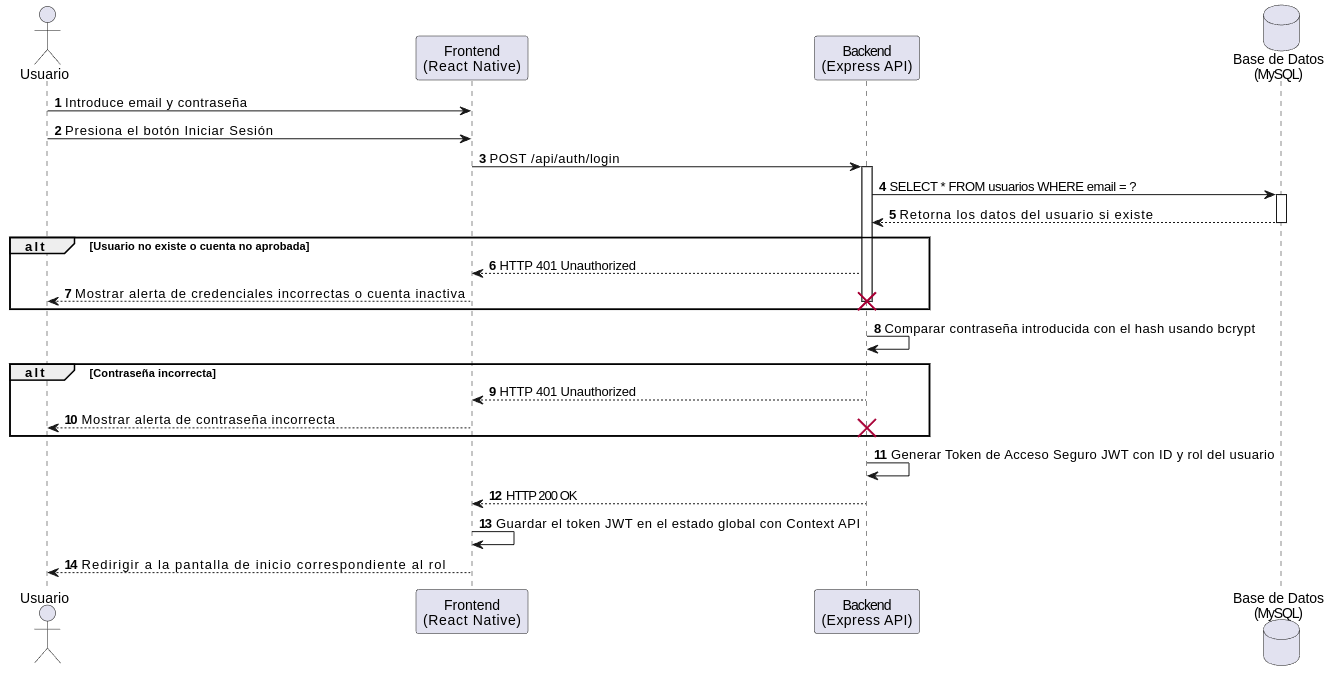
\includegraphics[width=1\textwidth]{diagramas/CU_05.drawio.png}
            \caption{Diagrama de secuencia del CU\_05.}
            \label{fig:seq_cu_05}
        \end{figure}  

        \begin{table}[htbp]
        \centering
        \footnotesize
        \renewcommand{\arraystretch}{1.0}
        \begin{tabularx}{\textwidth}{|l|X|}
        \hline
        \rowcolor[HTML]{EFEFEF} 
        \textbf{Caso de Uso} & \textbf{Modificación de contraseña (CU\_20)} \\ \hline
        \textbf{Actores} & General (Padre/Tutor legal, Entrenador y Administrador) \\ \hline
        \textbf{Tipo} & Primario y esencial. \\ \hline
        \textbf{Referencias} & RF1.7 \\ \hline
        \textbf{Precondición} & El usuario ha iniciado sesión con sus credenciales actuales. \\ \hline
        \textbf{Postcondición} & Los datos de contacto o la nueva contraseña se actualizan de forma persistente mediante hash en la base de datos MySQL. \\ \hline
        \textbf{Propósito} & Permitir a los usuarios modificar su contraseña. \\ \hline
        \textbf{Resumen} & El usuario accede a la sección de seguridad dentro de la aplicación móvil, introduce la nueva contraseña junto con su confirmación y el sistema valida, encripta y actualiza la credencial en la base de datos. \\ \hline
        \textbf{Curso Normal} & 
        \textbf{1.} El usuario accede al formulario de cambio de contraseña.\newline
        \textbf{2.} El sistema muestra los campos para introducir la nueva contraseña y su correspondiente confirmación.\newline
        \textbf{3.} El usuario introduce la nueva clave privada en ambos campos y presiona "Confirmar Cambio".\newline
        \textbf{4.} El frontend en React Native comprueba que la cadena de texto cumpla con los requisitos mínimos de longitud y coincidencia.\newline
        \textbf{5.} El backend en Node.js recibe la solicitud, valida la firma del token y procesa la nueva clave mediante el algoritmo \textit{bcrypt}.\newline
        \textbf{6.} El sistema ejecuta el query en MySQL actualizando el campo de la contraseña y cambia el estado de la cuenta a "validada".\newline
        \textbf{7.} La aplicación móvil redirige al usuario a la pantalla principal confirmando el éxito de la operación. \\ \hline
        \textbf{Cursos Alternos} & 
        \textbf{4a:} El sistema detecta en la interfaz que la contraseña y su confirmación no coinciden, interrumpe el envío al backend y muestra una alerta visual de error.\newline
        \textbf{6a:} El backend compara el hash y detecta que el usuario intenta reutilizar la misma clave temporal por defecto; deniega la actualización y solicita una combinación de caracteres diferente. \\ \hline
        \end{tabularx}
        \caption{Ficha caso de uso CU\_20.}
        \label{tab:cu_20}
        \end{table}

        \begin{table}[htbp]
        \centering
        \footnotesize
        \renewcommand{\arraystretch}{1.0}
        \begin{tabularx}{\textwidth}{|l|X|}
        \hline
        \rowcolor[HTML]{EFEFEF} 
        \textbf{Caso de Uso} & \textbf{Recuperar credenciales de acceso (CU\_22)} \\ \hline
        \textbf{Actores} & General (Padre/Tutor legal, Entrenador y Administrador) \\ \hline
        \textbf{Tipo} & Primario y esencial. \\ \hline
        \textbf{Referencias} & RF1.8, CU\_05 \\ \hline
        \textbf{Precondición} & El usuario está previamente registrado en el sistema, pero no recuerda sus credenciales de acceso. \\ \hline
        \textbf{Postcondición} & La contraseña anterior queda invalidada y la nueva clave se almacena encriptada de forma persistente en la base de datos MySQL. \\ \hline
        \textbf{Propósito} & Permitir a los usuarios restablecer su contraseña de forma autónoma y segura mediante la verificación de un código de validación enviado a su dirección de correo electrónico. \\ \hline
        \textbf{Resumen} & El usuario solicita la recuperación desde la pantalla de login introduciendo su correo electrónico. El sistema genera un código temporal y lo envía por email; tras introducir dicho código junto con la nueva contraseña, el sistema valida la transacción y actualiza las credenciales en la base de datos. \\ \hline
        \textbf{Curso Normal} & 
        \textbf{1.} El usuario abre la aplicación, selecciona la opción "Olvidé mi contraseña" e introduce su correo electrónico.\newline
        \textbf{2.} El backend verifica la existencia del correo en MySQL, genera un código de validación temporal y realiza el envío automático por email.\newline
        \textbf{3.} El usuario copia el código recibido en su buzón y accede al formulario de restablecimiento en la app.\newline
        \textbf{4.} El sistema habilita los campos para introducir el código de verificación, la nueva contraseña y su confirmación.\newline
        \textbf{5.} El usuario rellena los datos requeridos y presiona "Restablecer Contraseña".\newline
        \textbf{6.} El frontend comprueba que las cadenas de texto de las contraseñas coincidan.\newline
        \textbf{7.} El backend valida que el código introducido sea correcto. Encripta y guarda la nueva contraseña en la base de datos.\newline
        \textbf{8.} El sistema redirige al usuario a la pantalla de login original mostrando un mensaje de éxito. \\ \hline
        \textbf{Cursos Alternos} & 
        \textbf{2a:} El sistema detecta que el email introducido no coincide con ningún usuario en la base de datos. Interrumpe el flujo y muestra una alerta genérica en la interfaz por motivos de seguridad.\newline
        \textbf{6b:} El frontend detecta que la nueva contraseña y su confirmación no son idénticas y muestra un aviso de error.\newline
        \textbf{7b:} El backend comprueba que el código ingresado es incorrecto o que el tiempo límite del token ha caducado. Cancela la operación en MySQL y solicita al usuario demandar un nuevo código. \\ \hline
        \end{tabularx}
        \caption{Ficha caso de uso CU\_22.}
        \label{tab:cu_22}
        \end{table}

        \newpage
        \subsubsection{Módulo de planificación de entrenamientos}
        Este módulo gestiona el ciclo de vida de la programación deportiva del club, permitiendo la creación, modificación y consulta de sesiones de entrenamiento en nieve, competiciones y preparación física.
        
        \begin{figure}[htbp]
        \centering
        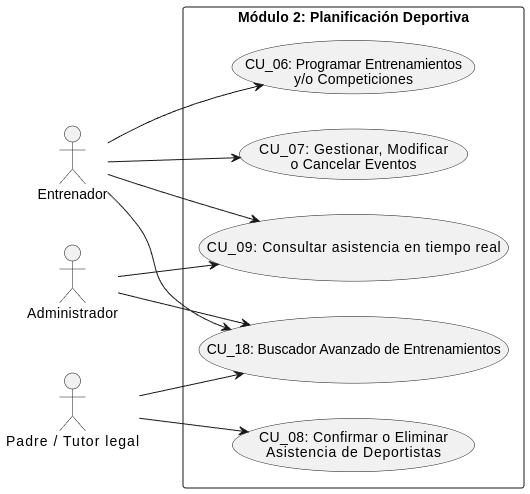
\includegraphics[width=1\textwidth]{diagramas/DiagramaPlanificacionEntrenos.drawio.png}
        \caption{Diagrama de planificación de entrenamientos.}
        \label{fig:diagrama_planificacion_entrenamientos}
        \end{figure}

        \begin{table}[htbp]
        \centering
        \footnotesize
        \renewcommand{\arraystretch}{0.95}
        \begin{tabularx}{\textwidth}{|l|X|}
        \hline
        \rowcolor[HTML]{EFEFEF} 
        \textbf{Caso de Uso} & \textbf{Programar entrenamientos y/o competiciones (CU\_06)} \\ \hline
        \textbf{Actores} & Entrenador \\ \hline
        \textbf{Tipo} & Primario y esencial \\ \hline
        \textbf{Referencias} & RF2.1, RF4.1 \\ \hline
        \textbf{Precondición} & El entrenador ha iniciado sesión y su cuenta está activa dentro de su categoría asignada. \\ \hline
        \textbf{Postcondición} & El evento se calendariza y se guarda de forma persistente en la tabla eventos de MySQL. \\ \hline
        \textbf{Propósito} & Permitir al personal técnico calendarizar una nueva sesión de entrenamiento, competición o preparación física. \\ \hline
        \textbf{Resumen} & El entrenador abre el módulo de planificación, introduce los detalles del evento (fecha, hora, lugar y plazas de transporte opcionales) y confirma. El sistema valida los datos y publica el evento en el calendario de las familias. \\ \hline
        \textbf{Curso Normal} & 
        \textbf{1.} El Entrenador accede al calendario y presiona Crear Evento.\newline
        \textbf{2.} El sistema muestra el formulario de creación solicitando los datos del evento.\newline
        \textbf{3.} El Entrenador rellena los campos.\newline
        \textbf{4.} El Entrenador confirma la creación del evento.\newline
        \textbf{5.} El sistema verifica que los campos obligatorios sean válidos y no tengan conflictos horarios.\newline
        \textbf{6.} El sistema almacena el registro en la base de datos y actualiza el calendario. \\ \hline
        \textbf{Cursos Alternos} & 
        \textbf{5a:} El sistema detecta que la fecha elegida es anterior a la fecha actual o faltan datos obligatorios. \\ \hline
        \end{tabularx}
        \caption{Ficha caso de uso CU\_06.}
        \label{tab:cu_06}
        \end{table}

        \begin{figure}[htbp]
            \centering
            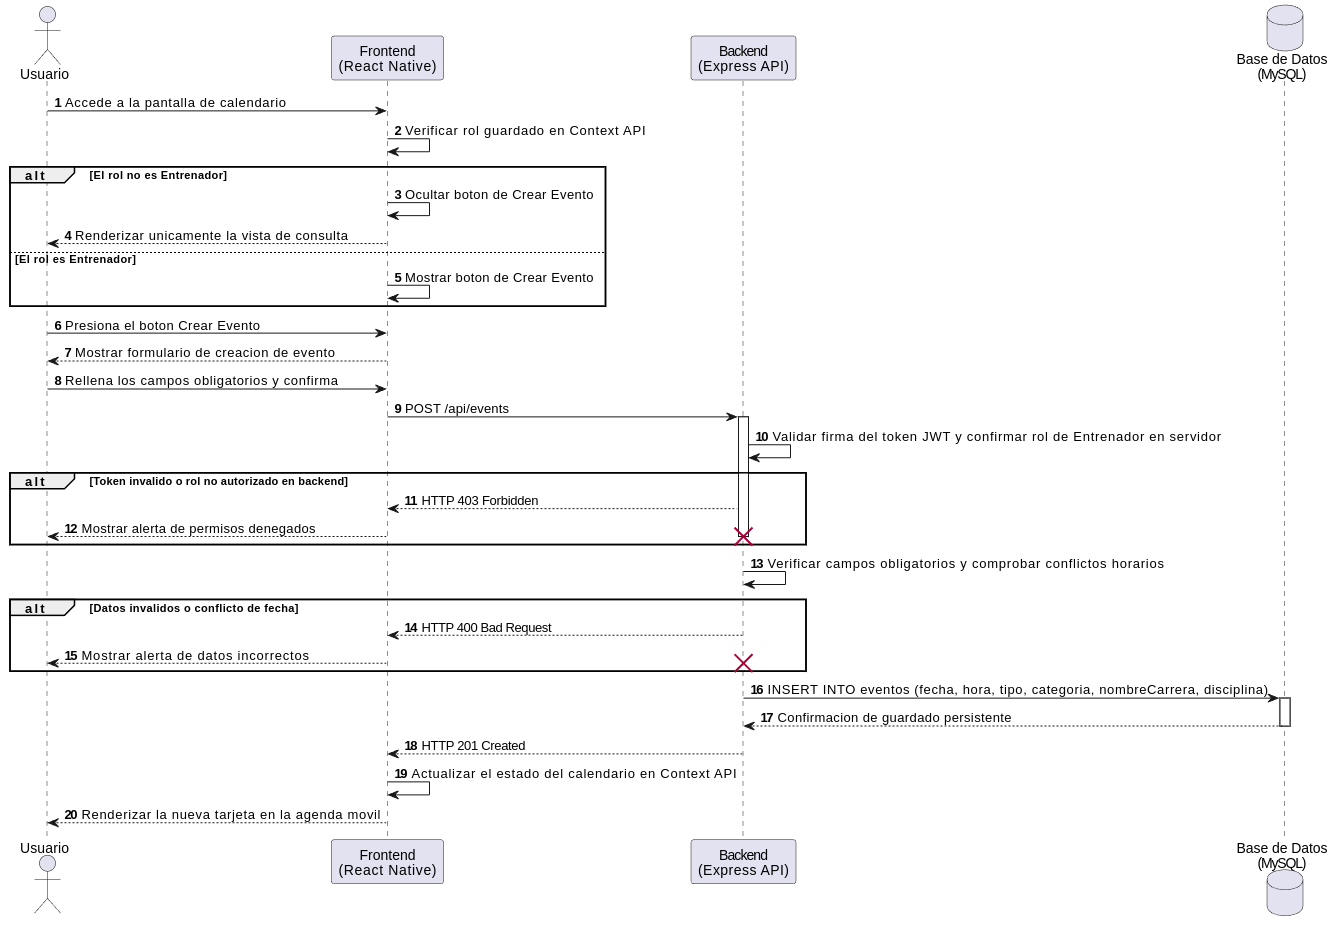
\includegraphics[width=1\textwidth]{diagramas/CU_06.drawio.png}
            \caption{Diagrama de secuencia del CU\_06.}
            \label{fig:seq_cu_06}
        \end{figure}

        \begin{table}[htbp]
        \centering
        \footnotesize
        \renewcommand{\arraystretch}{0.95}
        \begin{tabularx}{\textwidth}{|l|X|}
        \hline
        \rowcolor[HTML]{EFEFEF} 
        \textbf{Caso de Uso} & \textbf{Gestionar, modificar o cancelar eventos (CU\_07)} \\ \hline
        \textbf{Actores} & Entrenador \\ \hline
        \textbf{Tipo} & Primario y esencial. \\ \hline
        \textbf{Referencias} & RF2.4, RF4.1 y RF4.3 \\ \hline
        \textbf{Precondición} & El evento ya ha sido creado previamente por el entrenador y existe en la base de datos. \\ \hline
        \textbf{Postcondición} & El evento se actualiza o elimina en MySQL, y se notifica del cambio a los padres. \\ \hline
        \textbf{Propósito} & Permitir al personal técnico realizar modificaciones o cancelaciones en los entrenamientos ya programados debido a contingencias climáticas o logísticas. \\ \hline
        \textbf{Resumen} & El entrenador selecciona un evento de su calendario, modifica sus datos o pulsa en cancelar, y confirma la acción. El sistema actualiza la base de datos. \\ \hline
        \textbf{Curso Normal} & 
        \textbf{1.} El Entrenador accede a los detalles del entrenamiento y presiona ``Editar'' o ``Eliminar''.\newline
        \textbf{2.} El sistema muestra los datos actuales del evento permitiendo su edición o solicita confirmación de borrado.\newline
        \textbf{3.} El Entrenador modifica los datos necesarios (o confirma la cancelación) y presiona ``Guardar cambios''.\newline
        \textbf{4.} El sistema valida que los nuevos datos introducidos sean correctos.\newline
        \textbf{5.} El sistema actualiza el estado o la información del evento en la base de datos.\newline
        \textbf{6.} El sistema genera una notificación automática para avisar a los padres vinculados sobre el cambio. \\ \hline
        \textbf{Cursos Alternos} & 
        \textbf{4a:} El sistema detecta que la nueva fecha u hora introducida es inválida o anterior al día de hoy. \\ \hline
        \end{tabularx}
        \caption{Ficha caso de uso CU\_07.}
        \label{tab:cu_07}
        \end{table}

        \begin{figure}[htbp]
            \centering
            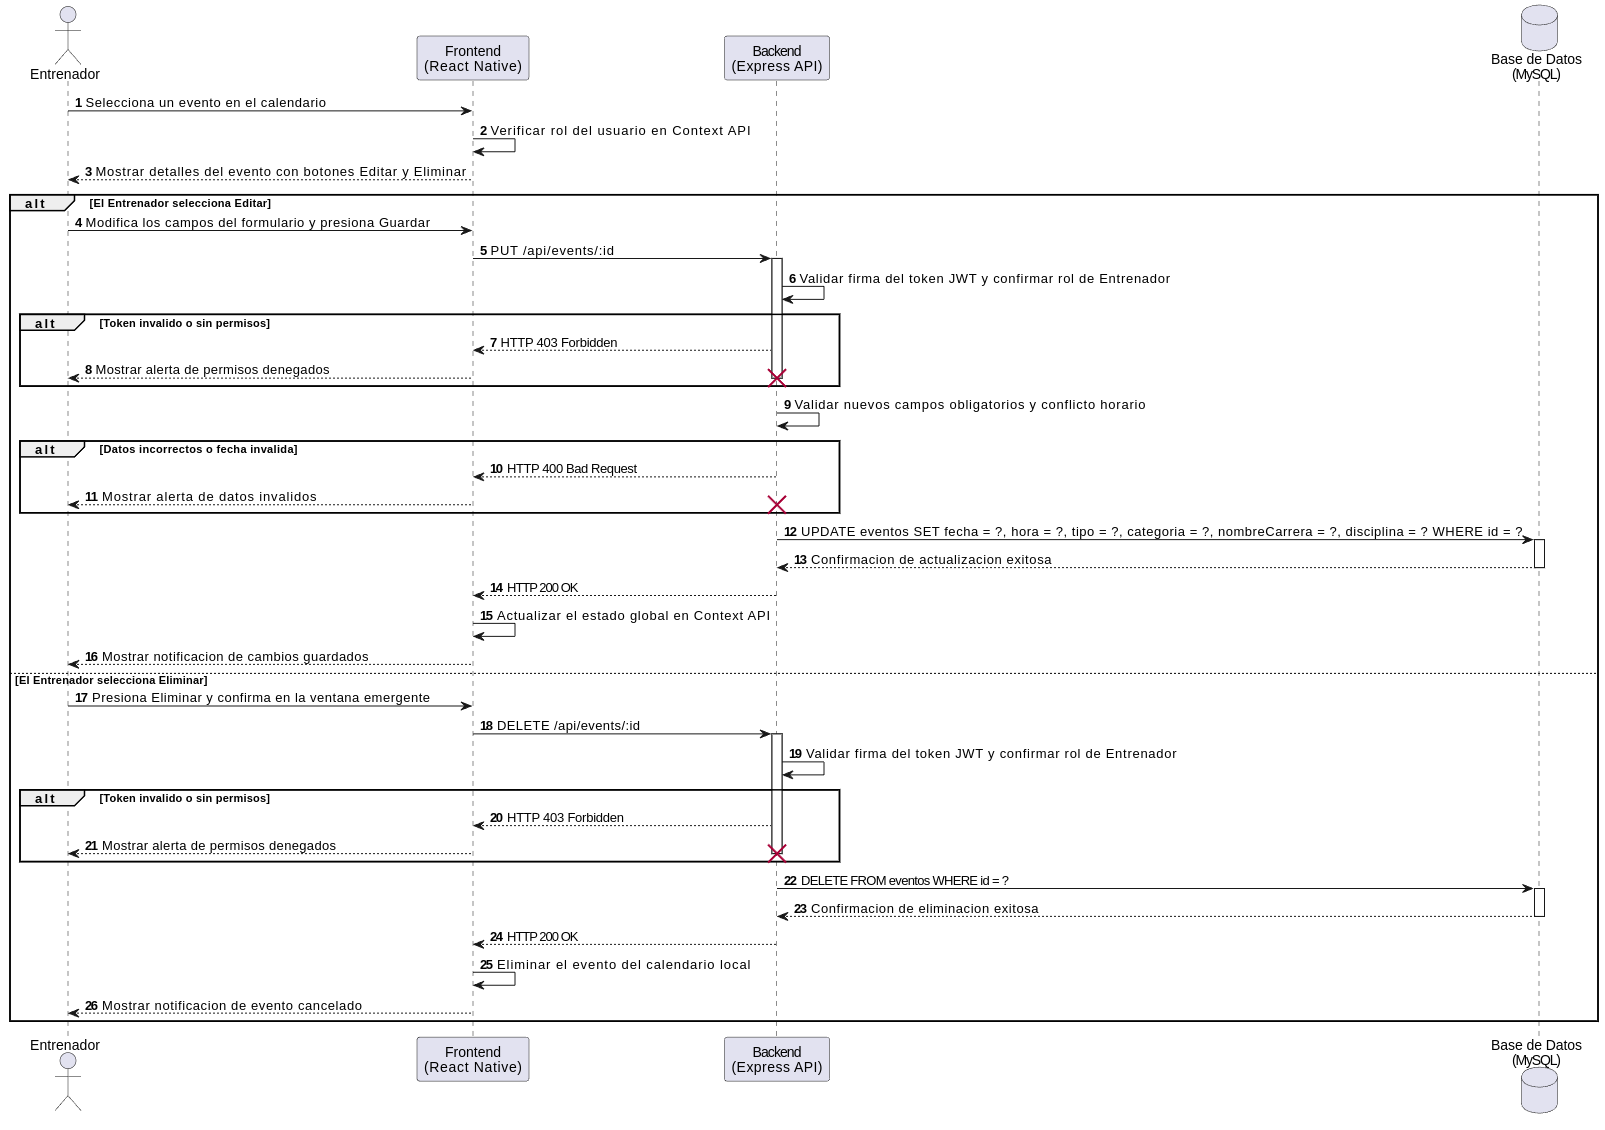
\includegraphics[width=0.8\textwidth]{diagramas/CU_07.drawio.png}
            \caption{Diagrama de secuencia del CU\_07.}
            \label{fig:seq_cu_07}
        \end{figure}

        \begin{table}[htbp]
        \centering
        \footnotesize
        \renewcommand{\arraystretch}{0.95}
        \begin{tabularx}{\textwidth}{|l|X|}
        \hline
        \rowcolor[HTML]{EFEFEF} 
        \textbf{Caso de Uso} & \textbf{Confirmar o eliminar la asistencia (CU\_08)} \\ \hline
        \textbf{Actores} & Padre / Tutor legal \\ \hline
        \textbf{Tipo} & Primario y esencial. \\ \hline
        \textbf{Referencias} & RF2.2, RF4.2 \\ \hline
        \textbf{Precondición} & El entrenador ha publicado un evento con transporte vinculado y el padre tiene a sus hijos registrados. \\ \hline
        \textbf{Postcondición} & Se actualiza el estado de asistencia y se reserva (o libera) la plaza de furgoneta en MySQL. \\ \hline
        \textbf{Propósito} & Permitir a los padres gestionar la asistencia de sus hijos a los entrenamientos y reservar su plaza en el transporte del club simultáneamente. \\ \hline
        \textbf{Resumen} & El padre selecciona un evento, marca la asistencia de su hijo junto con la opción de transporte y confirma. El sistema comprueba el aforo, procesa el cambio y actualiza la base de datos. \\ \hline
        \textbf{Curso Normal} & 
        \textbf{1.} El Padre accede al calendario de la app móvil y selecciona un entrenamiento.\newline
        \textbf{2.} El sistema muestra los detalles del evento, los nombres de sus hijos y la opción de transporte.\newline
        \textbf{3.} El Padre marca la casilla de asistencia, activa el check de ``Reserva de Transporte'' y presiona ``Guardar''.\newline
        \textbf{4.} El sistema verifica de forma activa que queden plazas libres en el vehículo para ese viaje.\newline
        \textbf{5.} El sistema registra la asistencia del menor y descuenta una plaza del aforo del transporte en la base de datos.\newline
        \textbf{6.} El sistema refresca la pantalla confirmando que la asistencia y la furgoneta se han reservado con éxito. \\ \hline
        \textbf{Cursos Alternos} & 
        \textbf{4a:} El sistema detecta que el transporte ya ha alcanzado el límite de capacidad máxima. Inscribe al niño solo en la asistencia en pista y muestra una alerta informando que ya no quedan plazas libres en el vehículo. \\ \hline
        \end{tabularx}
        \caption{Ficha caso de uso CU\_08.}
        \label{tab:cu_08}
        \end{table}

        \begin{figure}[htbp]
            \centering
            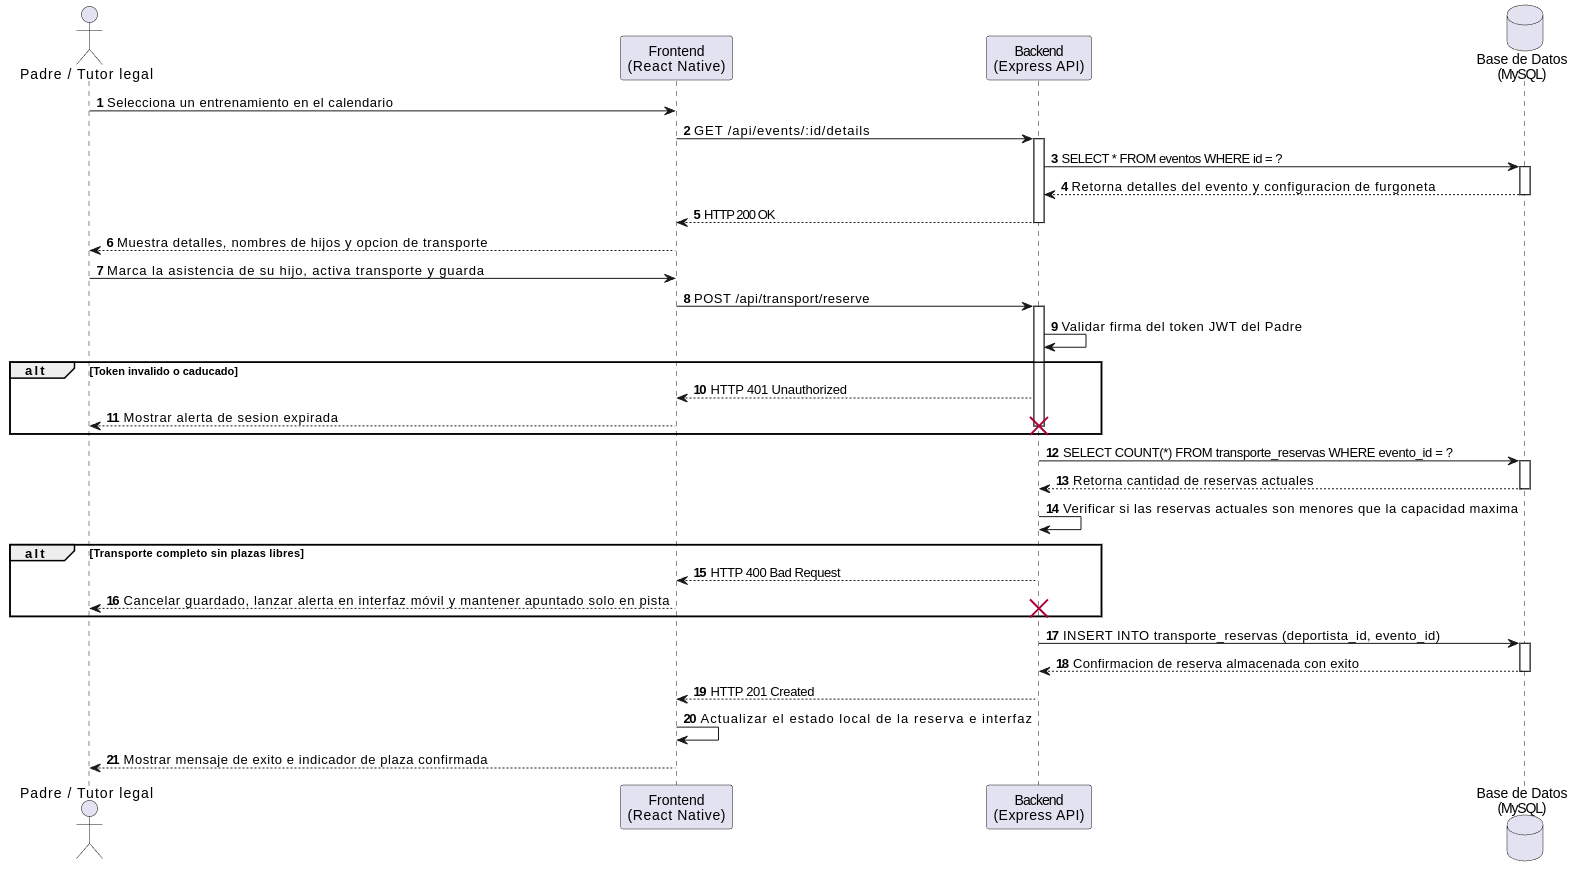
\includegraphics[width=0.9\textwidth]{diagramas/CU_08.drawio.png}
            \caption{Diagrama de secuencia del CU\_08.}
            \label{fig:seq_cu_08}
        \end{figure}

        \begin{table}[htbp]
        \centering
        \footnotesize
        \renewcommand{\arraystretch}{0.85}
        \begin{tabularx}{\textwidth}{|l|X|}
        \hline
        \rowcolor[HTML]{EFEFEF} 
        \textbf{Caso de Uso} & \textbf{Consultar el listado de asistencia (CU\_09)} \\ \hline
        \textbf{Actores} & Entrenador \\ \hline
        \textbf{Tipo} & Primario y esencial. \\ \hline
        \textbf{Referencias} & RF2.3, RF4.2 \\ \hline
        \textbf{Precondición} & El entrenador ha iniciado sesión y existen registros de asistencia para ese evento. \\ \hline
        \textbf{Postcondición} & El entrenador visualiza en tiempo real el listado consolidado de deportistas apuntados. \\ \hline
        \textbf{Propósito} & Permitir al personal técnico consultar de manera centralizada la lista de menores que asistirán y verificar el transporte. \\ \hline
        \textbf{Resumen} & El entrenador selecciona un evento de su calendario. El sistema consulta en MySQL y devuelve el listado con indicadores de transporte en la app móvil. \\ \hline
        \textbf{Curso Normal} & 
        \textbf{1.} El Entrenador accede a la agenda y selecciona un entrenamiento específico.\newline
        \textbf{2.} El Entrenador presiona la opción ``Ver Lista de Asistencia''.\newline
        \textbf{3.} El frontend realiza una petición GET al backend enviando el ID del evento y el token de sesión.\newline
        \textbf{4.} El backend valida el token e interroga a MySQL mediante un JOIN entre asistencia, deportistas y transporte.\newline
        \textbf{5.} El sistema retorna el listado de alumnos indicando quiénes tienen plaza reservada en la furgoneta.\newline
        \textbf{6.} La aplicación móvil genera la lista de forma visual en la pantalla del entrenador. \\ \hline
        \textbf{Cursos Alternos} & 
        \textbf{4a:} No hay asistencias confirmadas todavía: el sistema devuelve una estructura vacía y muestra un aviso informativo. \\ \hline
        \end{tabularx}
        \caption{Ficha caso de uso CU\_09.}
        \label{tab:cu_09}
        \end{table}

        \begin{table}[htbp]
        \centering
        \footnotesize
        \renewcommand{\arraystretch}{0.85}
        \begin{tabularx}{\textwidth}{|l|X|}
        \hline
        \rowcolor[HTML]{EFEFEF} 
        \textbf{Caso de Uso} & \textbf{Consultar entrenamientos (CU\_18)} \\ \hline
        \textbf{Actores} & Padre / Tutor legal \\ \hline
        \textbf{Tipo} & Primario y esencial. \\ \hline
        \textbf{Referencias} & RF4.1 \\ \hline
        \textbf{Precondición} & El usuario ha iniciado sesión en la aplicación móvil. \\ \hline
        \textbf{Postcondición} & El usuario visualiza la planificación de entrenamientos y competiciones en el calendario. \\ \hline
        \textbf{Propósito} & Permitir a los padres consultar los días, horarios y disciplinas asignadas para las sesiones de sus hijos. \\ \hline
        \textbf{Resumen} & El usuario accede a la vista de calendario en la app móvil. El sistema consulta en MySQL filtrando por los deportistas vinculados al tutor y muestra los eventos. \\ \hline
        \textbf{Curso Normal} & 
        \textbf{1.} El Padre accede al apartado de ``Calendario'' desde el menú principal de la aplicación móvil.\newline
        \textbf{2.} La app envía una solicitud GET al backend solicitando los eventos programados para las categorías de sus hijos.\newline
        \textbf{3.} El backend recibe la solicitud, valida el token JWT y realiza la consulta en la base de datos MySQL.\newline
        \textbf{4.} El sistema retorna un listado con los detalles de los entrenamientos (fecha, hora, disciplina y ubicación).\newline
        \textbf{5.} La aplicación móvil recibe los datos y los genera de forma ordenada en la interfaz del calendario. \\ \hline
        \textbf{Cursos Alternos} & 
        \textbf{4a:} No existen eventos programados para las categorías asociadas al usuario: el sistema devuelve una estructura vacía y muestra el mensaje correspondiente. \\ \hline
        \end{tabularx}
        \caption{Ficha caso de uso CU\_18.}
        \label{tab:cu_18}
        \end{table}        
        \newpage
        \subsubsection{Módulo de gestión de logística y transporte}
        Este módulo coordina la asignación, reserva y liberación de plazas limitadas en los vehículos del club, implementando validaciones de concurrencia en el backend para controlar los aforos en tiempo real y asegurar la integridad de las reservas en la base de datos MySQL.
        \begin{figure}[htbp]
            \centering
            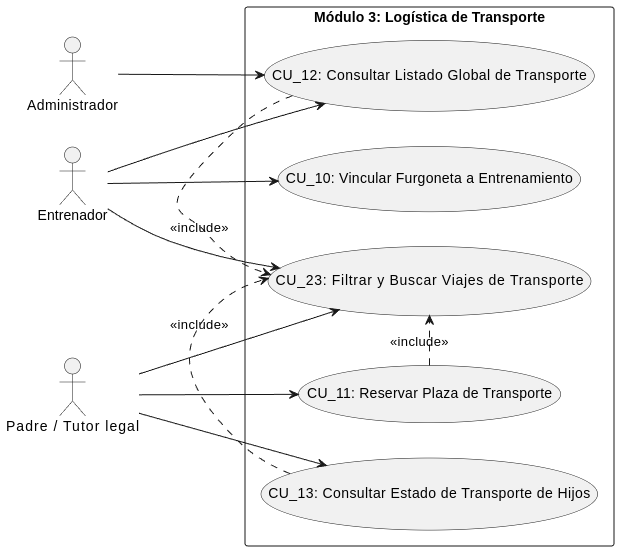
\includegraphics[width=0.6\textwidth]{diagramas/DiagramaLogisticaTransporte.drawio.png}
            \caption{Diagrama de gestión de transporte.}
            \label{fig:diagrama_gestion_transporte}
        \end{figure}
        \newline
        \newline
        \newline
        \newline
        \newline
        \newline
        \newline
        \newline
        \newline
        \newline
        \newline
        \newline
        \newline
        \newline

        \begin{table}[htbp]
        \centering
        \footnotesize
        \renewcommand{\arraystretch}{0.95}
        \begin{tabularx}{\textwidth}{|l|X|}
        \hline
        \rowcolor[HTML]{EFEFEF} 
        \textbf{Caso de Uso} & \textbf{Modificar capacidad del transporte (CU\_10)} \\ \hline
        \textbf{Actores} & Administrador \\ \hline
        \textbf{Tipo} & Primario y esencial. \\ \hline
        \textbf{Ref} & RF4.2 \\ \hline
        \textbf{Precondicion} & El administrador ha iniciado sesión y el transporte está registrado en el sistema. \\ \hline
        \textbf{Postcondicion} & La nueva capacidad de plazas queda actualizada de forma persistente en la base de datos MySQL. \\ \hline
        \textbf{Propósito} & Permitir la modificación del número máximo de plazas disponibles en el transporte del club. \\ \hline
        \textbf{Resumen} & El administrador accede al módulo de transporte, edita el número de plazas asignadas a un vehículo y confirma el cambio. El sistema valida la información y actualiza el aforo en MySQL. \\ \hline
        \textbf{Curso Normal} & 
        \textbf{1.} El Administrador accede al apartado de gestión de transporte en el panel de administración.\newline
        \textbf{2.} El sistema muestra los datos del transporte actual junto con el campo de capacidad de plazas.\newline
        \textbf{3.} El Administrador introduce el nuevo número de plazas disponibles y presiona ``Guardar''.\newline
        \textbf{4.} El backend recibe la petición, valida el token JWT del administrador y comprueba que el valor sea un número entero válido.\newline
        \textbf{5.} El sistema ejecuta la actualización en la base de datos MySQL reflejando el nuevo aforo.\newline
        \textbf{6.} El panel de administración web refresca los datos confirmando que la capacidad se ha actualizado con éxito. \\ \hline
        \textbf{Cursos Alternos} & 
        \textbf{4a:} El Administrador introduce un valor negativo o vacío: el sistema interrumpe la operación y muestra un mensaje de error en la interfaz. \\ \hline
        \end{tabularx}
        \caption{Ficha caso de uso CU\_10.}
        \label{tab:cu_10}
        \end{table}

        \begin{figure}[htbp]
            \centering
            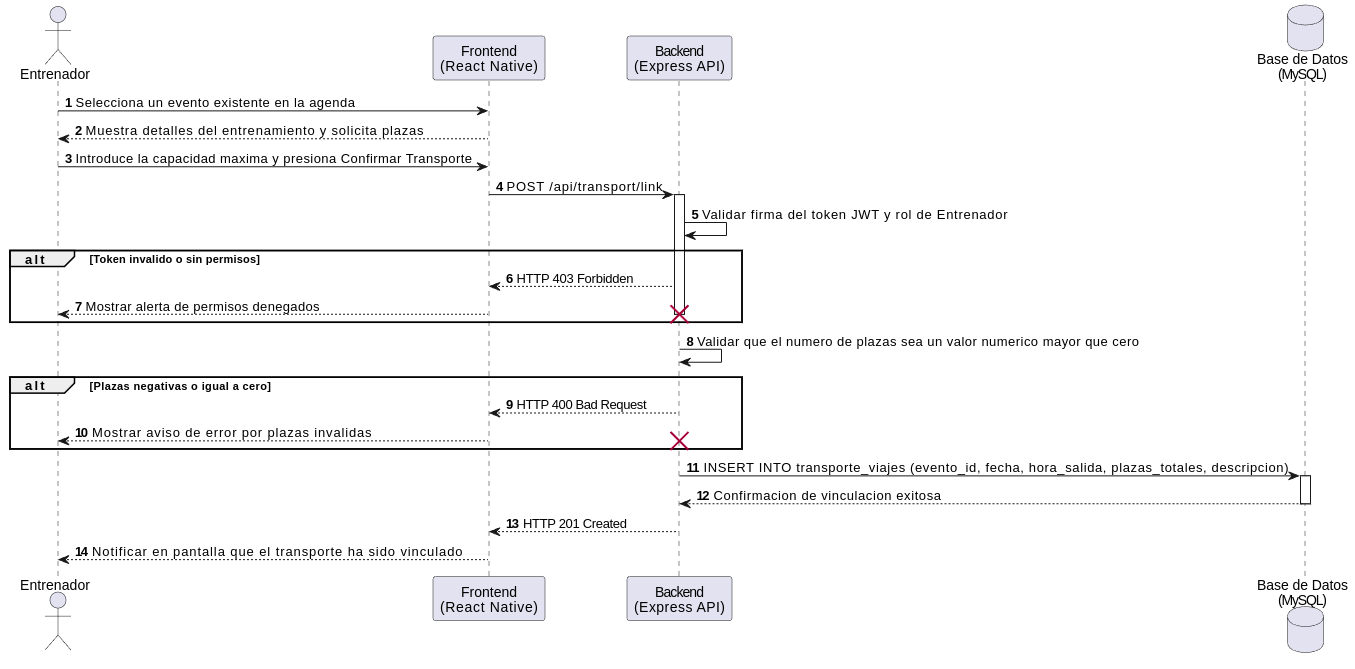
\includegraphics[width=1\textwidth]{diagramas/CU_10.drawio.png}
            \caption{Diagrama de secuencia del CU\_10.}
            \label{fig:seq_cu_10}
        \end{figure}

        \begin{table}[htbp]
        \centering
        \footnotesize
        \renewcommand{\arraystretch}{0.95}
        \begin{tabularx}{\textwidth}{|l|X|}
        \hline
        \rowcolor[HTML]{EFEFEF} 
        \textbf{Caso de Uso} & \textbf{Reservar plaza de transporte (CU\_11)} \\ \hline
        \textbf{Actores} & Padre/tutor legal \\ \hline
        \textbf{Tipo} & Primario y esencial \\ \hline
        \textbf{Referencias} & RF4.2, RF4.3 \\ \hline
        \textbf{Precondición} & El entrenador ha vinculado previamente una furgoneta al entrenamiento y el menor está confirmado para asistir al entrenamiento. \\ \hline
        \textbf{Postcondición} & Se crea el registro de reserva en MySQL y se decrementa una plaza disponible en el aforo del vehículo. \\ \hline
        \textbf{Propósito} & Permitir a los padres asegurar un asiento en el vehículo del club para el traslado de sus hijos a la estación de esquí, garantizando que no se supere la capacidad máxima del vehículo. \\ \hline
        \textbf{Resumen} & El padre accede al detalle del entrenamiento en la aplicación móvil, activa la opción de transporte y confirma. El sistema comprueba el aforo disponible en tiempo real, bloquea la plaza y actualiza la base de datos. \\ \hline
        \textbf{Curso Normal} & 
        \textbf{1.} El Padre accede al evento programado dentro de su calendario en la aplicación móvil.\newline
        \textbf{2.} El sistema comprueba si el evento tiene transporte asociado y solicita al backend el aforo disponible.\newline
        \textbf{3.} El Padre marca la casilla ``Reservar Plaza en Furgoneta'' y presiona el botón ``Confirmar''.\newline
        \textbf{4.} El sistema verifica en la base de datos (MySQL) que el número de reservas actuales sea estrictamente menor que la capacidad máxima permitida.\newline
        \textbf{5.} El sistema almacena la reserva del alumno de forma persistente en la tabla \textit{transporte\_reservas}.\newline
        \textbf{6.} El sistema actualiza la interfaz en React Native mostrando un mensaje de éxito y el indicador de plaza confirmada. \\ \hline
        \textbf{Cursos Alternos} & 
        \textbf{4a:} El sistema detecta que el número de reservas ha alcanzado el límite de capacidad de la furgoneta. Cancela el proceso de guardado, lanza una alerta en la interfaz móvil informando de que ya no quedan asientos libres y mantiene al deportista apuntado únicamente al entrenamiento. \\ \hline
        \end{tabularx}
        \caption{Ficha caso de uso CU\_11.}
        \label{tab:cu_11_reserva}
        \end{table}

        \clearpage

        \begin{table}[htbp]
        \centering
        \footnotesize
        \renewcommand{\arraystretch}{0.85}
        \begin{tabularx}{\textwidth}{|l|X|}
        \hline
        \rowcolor[HTML]{EFEFEF} 
        \textbf{Caso de Uso} & \textbf{Consultar listado global de transporte (CU\_12)} \\ \hline
        \textbf{Actores} & Entrenador, administrador \\ \hline
        \textbf{Tipo} & Primario y esencial \\ \hline
        \textbf{Referencias} & RF4.3, RF4.4 \\ \hline
        \textbf{Precondición} & El usuario ha iniciado sesión y existen reservas de plazas confirmadas por los padres para el viaje. \\ \hline
        \textbf{Postcondición} & El sistema muestra en pantalla la hoja con todos los pasajeros asignados al vehículo. \\ \hline
        \textbf{Propósito} & Permitir al personal técnico controlar el aforo total y la lista de menores que viajan en la furgoneta en un entrenamiento específico. \\ \hline
        \textbf{Resumen} & El usuario accede al apartado de transporte. El sistema realiza una consulta relacional y genera la lista de deportistas con plaza reservada. \\ \hline
        \textbf{Curso Normal} & 
        \textbf{1.} El usuario accede al menú de logística del transporte y selecciona un viaje programado.\newline
        \textbf{2.} El usuario presiona el botón de ``Logística de furgoneta''.\newline
        \textbf{3.} El backend ejecuta la consulta en MySQL uniendo las tablas de reservas y deportistas sin aplicar filtros.\newline
        \textbf{4.} El sistema renderiza en la pantalla de la aplicación móvil el listado consolidado de todos los pasajeros confirmados. \\ \hline
        \textbf{Cursos Alternos} & 
        \textbf{3a:} El sistema detecta que ningún padre ha solicitado plaza para este trayecto y muestra la lista vacía con un aviso de 0 deportistas apuntados. \\ \hline
        \end{tabularx}
        \caption{Ficha caso de uso CU\_12.}
        \label{tab:cu_12}
        \end{table}

        \begin{figure}[htbp]
            \centering
            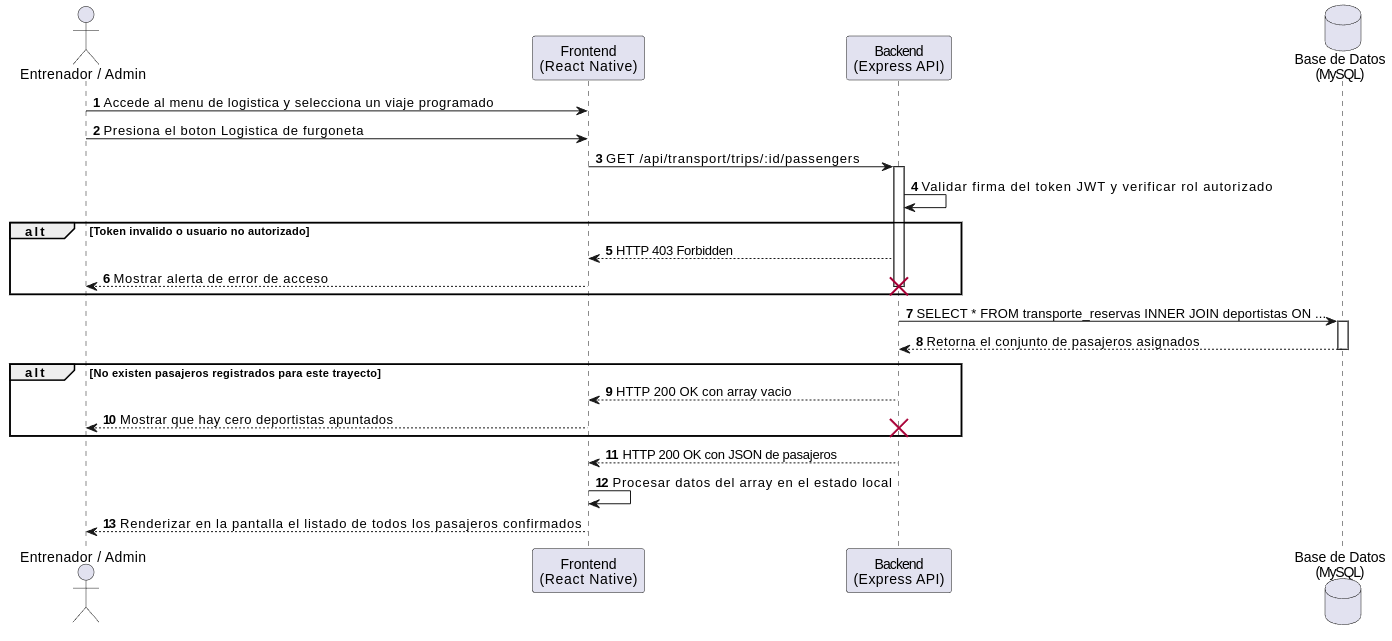
\includegraphics[width=0.8\textwidth]{diagramas/CU_12.drawio.png}
            \caption{Diagrama de secuencia del CU\_12.}
            \label{fig:seq_cu_12}
        \end{figure}

        \begin{table}[htbp]
        \centering
        \scriptsize
        \renewcommand{\arraystretch}{0.78}
        \begin{tabularx}{\textwidth}{|l|X|}
        \hline
        \rowcolor[HTML]{EFEFEF} 
        \textbf{Caso de Uso} & \textbf{Consultar estado de transporte de hijos (CU\_13)} \\ \hline
        \textbf{Actores} & Padre/tutor legal \\ \hline
        \textbf{Tipo} & Primario y esencial. \\ \hline
        \textbf{Referencias} & RF4.2, RF4.3 \\ \hline
        \textbf{Precondición} & El padre ha iniciado sesión y tiene solicitudes de reserva previas para los menores bajo su tutela. \\ \hline
        \textbf{Postcondición} & El sistema muestra únicamente el estado de las plazas solicitadas por el núcleo familiar. \\ \hline
        \textbf{Propósito} & Permitir a los padres verificar de forma privada si las plazas de furgoneta de sus hijos están asignadas. \\ \hline
        \textbf{Resumen} & El padre accede a transporte. El sistema lee su identidad mediante el token JWT, filtra en MySQL por sus hijos vinculados y genera los estados de reserva en la interfaz. \\ \hline
        \textbf{Curso Normal} & 
        \textbf{1.} El Padre accede al apartado de ``Mis Reservas de Transporte'' en la aplicación móvil.\newline
        \textbf{2.} El sistema extrae el ID del padre del token JWT almacenado en el estado global (Context API).\newline
        \textbf{3.} El Padre selecciona el entrenamiento que desea revisar.\newline
        \textbf{4.} El backend en Node.js realiza la consulta en MySQL filtrando por las plazas asociadas a los menores vinculados.\newline
        \textbf{5.} El sistema actualiza React Native mostrando el historial y estado (``Confirmado'' o ``No Confirmado'') de sus hijos. \\ \hline
        \textbf{Cursos Alternos} & 
        \textbf{4a:} No hay solicitudes vigentes: el sistema muestra un panel informativo con el texto ``No tienes reservas programadas''. \\ \hline
        \end{tabularx}
        \caption{Ficha caso de uso CU\_13.}
        \label{tab:cu_13}
        \end{table}

        \begin{table}[htbp]
        \centering
        \scriptsize
        \renewcommand{\arraystretch}{0.78}
        \begin{tabularx}{\textwidth}{|l|X|}
        \hline
        \rowcolor[HTML]{EFEFEF} 
        \textbf{Caso de Uso} & \textbf{Filtrar y buscar viajes de transporte (CU\_23)} \\ \hline
        \textbf{Actores} & General (Padre / Tutor legal, Entrenador y Administrador). \\ \hline
        \textbf{Tipo} & Primario y esencial \\ \hline
        \textbf{Referencias} & RF4.3, RF4.4 \\ \hline
        \textbf{Precondición} & El usuario ha iniciado sesión en la app y se encuentra en el módulo de administrar transporte. \\ \hline
        \textbf{Postcondición} & El sistema actualiza la interfaz mostrando las furgonetas y plazas que coinciden con los criterios. \\ \hline
        \textbf{Propósito} & Permitir restringir el listado de traslados seleccionando un rango de fechas o meses, evitando el desplazamiento infinito. \\ \hline
        \textbf{Resumen} & El usuario interactúa con los selectores temporales. El sistema captura las fechas, realiza una petición filtrada al backend y actualiza el estado local de React Native para renderizar las tarjetas. \\ \hline
        \textbf{Curso Normal} & 
        \textbf{1.} El usuario accede al menú de administración de transporte.\newline
        \textbf{2.} El sistema renderiza los selectores de búsqueda.\newline
        \textbf{3.} El usuario selecciona un mes o fecha concreta en la interfaz y pulsa el botón de filtrar.\newline
        \textbf{4.} El backend recibe los parámetros y ejecuta una consulta indexada en MySQL sobre la tabla de transporte.\newline
        \textbf{5.} El sistema devuelve la información de los viajes, aforos y estados de reserva que cumplen el criterio.\newline
        \textbf{6.} El frontend actualiza el estado local y refresca la pantalla mostrando únicamente las tarjetas coincidentes. \\ \hline
        \textbf{Cursos Alternos} & 
        \textbf{4a:} No existen viajes planificados en el periodo: el sistema limpia el listado y muestra un aviso de ausencia de registros. \\ \hline
        \end{tabularx}
        \caption{Ficha caso de uso CU\_23.}
        \label{tab:cu_23}
        \end{table}
        \newpage

        \subsubsection{Módulo de control de asistencia y rendimiento.}
        Este módulo gestiona el registro de la presencialidad de los deportistas en las sesiones de entrenamiento y competiciones, sirviendo como núcleo de datos para el análisis del progreso deportivo.
        \begin{figure}[htbp]
            \centering
            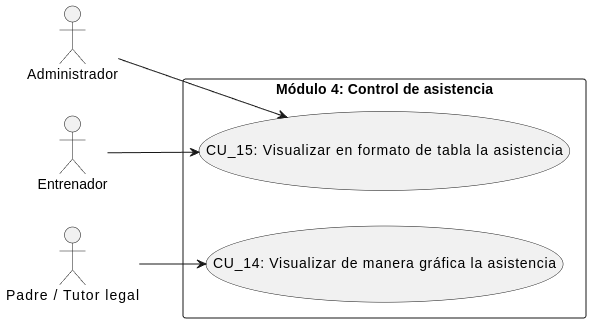
\includegraphics[width=0.8\textwidth]{diagramas/DiagramaAsistencia.drawio.png}
            \caption{Diagrama de control de asistencia.}
            \label{fig:diagrama_control_asistencia}
        \end{figure}

        \newpage

        \begin{table}[htbp]
        \centering
        \footnotesize
        \renewcommand{\arraystretch}{0.95}
        \begin{tabularx}{\textwidth}{|l|X|}
        \hline
        \rowcolor[HTML]{EFEFEF} 
        \textbf{Caso de Uso} & \textbf{Visualizar de manera gráfica la asistencia (CU\_14)} \\ \hline
        \textbf{Actores} & Padre/Tutor legal \\ \hline
        \textbf{Tipo} & Primario y esencial. \\ \hline
        \textbf{Referencias} & RF5.1, RF5.2, RF5.3, RF5.4 \\ \hline
        \textbf{Precondición} & El padre ha iniciado sesión y existen registros de asistencia guardados en el histórico de sus hijos. \\ \hline
        \textbf{Postcondición} & El sistema genera el componente gráfico en la pantalla del dispositivo móvil. \\ \hline
        \textbf{Propósito} & Permitir a los padres consultar de forma visual, intuitiva y rápida la progresión y regularidad de asistencia de sus hijos a los entrenamientos. \\ \hline
        \textbf{Resumen} & El padre accede al panel de asistencia de su hijo. El sistema solicita los datos acumulados al backend y genera un gráfico estadístico en la pantalla utilizando la librería de diseño. \\ \hline
        \textbf{Curso Normal} & 
        \textbf{1.} El Padre accede al perfil de su hijo y selecciona la pestaña ``Asistencia a los entrenamientos''.\newline
        \textbf{2.} El sistema solicita al backend las métricas de asistencia filtradas por el ID del deportista.\newline
        \textbf{3.} El backend procesa los datos en MySQL y devuelve un JSON con los porcentajes mensuales.\newline
        \textbf{4.} El sistema procesa los datos en el frontend y renderiza un gráfico dinámico (\textit{pie chart}) en la interfaz móvil. \\ \hline
        \textbf{Cursos Alternos} & 
        \textbf{3a:} El sistema detecta que el deportista no se ha apuntado a ningún entrenamiento y muestra que hay 0 \% de asistencia. \\ \hline
        \end{tabularx}
        \caption{Ficha caso de uso CU\_14.}
        \label{tab:cu_14}
        \end{table}

        \begin{figure}[htbp]
            \centering
            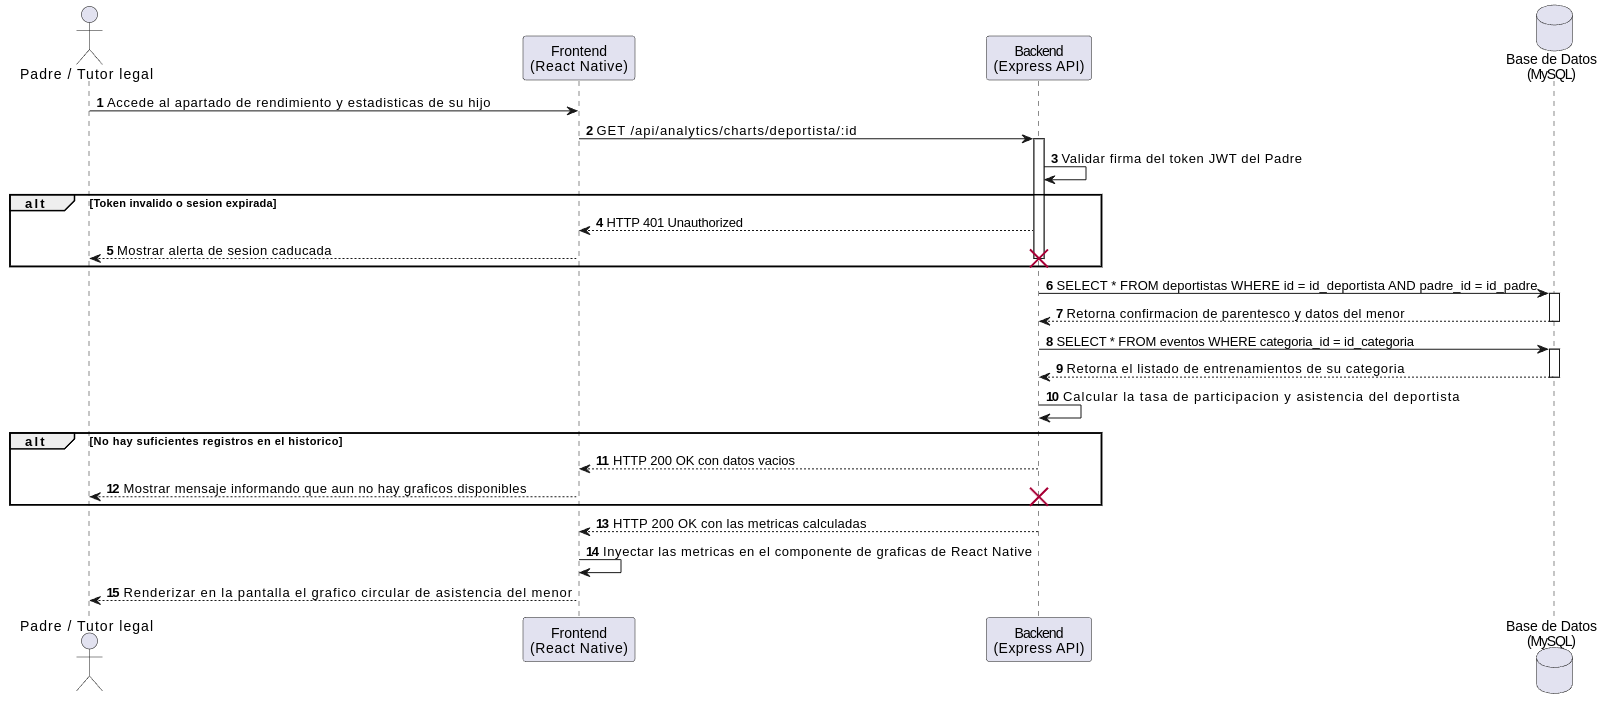
\includegraphics[width=0.8\textwidth]{diagramas/CU_14.drawio.png}
            \caption{Diagrama de secuencia del CU\_14.}
            \label{fig:seq_cu_14}
        \end{figure}

        \begin{table}[htbp]
        \centering
        \footnotesize
        \renewcommand{\arraystretch}{0.95}
        \begin{tabularx}{\textwidth}{|l|X|}
        \hline
        \rowcolor[HTML]{EFEFEF} 
        \textbf{Caso de Uso} & \textbf{Visualizar en formato de tabla la asistencia (CU\_15)} \\ \hline
        \textbf{Actores} & Entrenador, administrador. \\ \hline
        \textbf{Tipo} & Primario y esencial. \\ \hline
        \textbf{Referencias} & RF5.1, RF5.3, RF5.5, RF5.6 \\ \hline
        \textbf{Precondición} & El empleado ha iniciado sesión y pertenece a una categoría con deportistas en activo. \\ \hline
        \textbf{Postcondición} & El sistema muestra una matriz de datos detallada con el desglose de asistencia del grupo. \\ \hline
        \textbf{Propósito} & Permitir al personal técnico y de administración analizar los datos puros y exactos de asistencia de todo un grupo. \\ \hline
        \textbf{Resumen} & El entrenador o administrador selecciona una categoría y un mes. El sistema consulta la base de datos y genera una tabla cuadriculada con los nombres de los deportistas y sus días de asistencia y faltas. \\ \hline
        \textbf{Curso Normal} & 
        \textbf{1.} El Entrenador/Admin accede al módulo de ``Asistencia a los entrenos''.\newline
        \textbf{2.} El sistema muestra los filtros de selección por categoría deportiva y rango de fechas.\newline
        \textbf{3.} El Actor selecciona la categoría que desea auditar y confirma la consulta.\newline
        \textbf{4.} El backend ejecuta una consulta relacional pesada en MySQL para traer todo el histórico del grupo.\newline
        \textbf{5.} El sistema procesa la información y renderiza en pantalla una tabla organizada por filas (deportistas) y columnas (fechas/estados). \\ \hline
        \textbf{Cursos Alternos} & 
        \textbf{4a:} El sistema detecta que la categoría deportiva seleccionada no tiene entrenamientos registrados en el rango de fechas elegido.\newline
        \textbf{4b:} El sistema detiene la generación de la tabla y muestra un mensaje informativo en la pantalla: ``No existen datos de asistencia para los filtros seleccionados''. \\ \hline
        \end{tabularx}
        \caption{Ficha caso de uso CU\_15.}
        \label{tab:cu_15}
        \end{table}

        \begin{figure}[htbp]
            \centering
            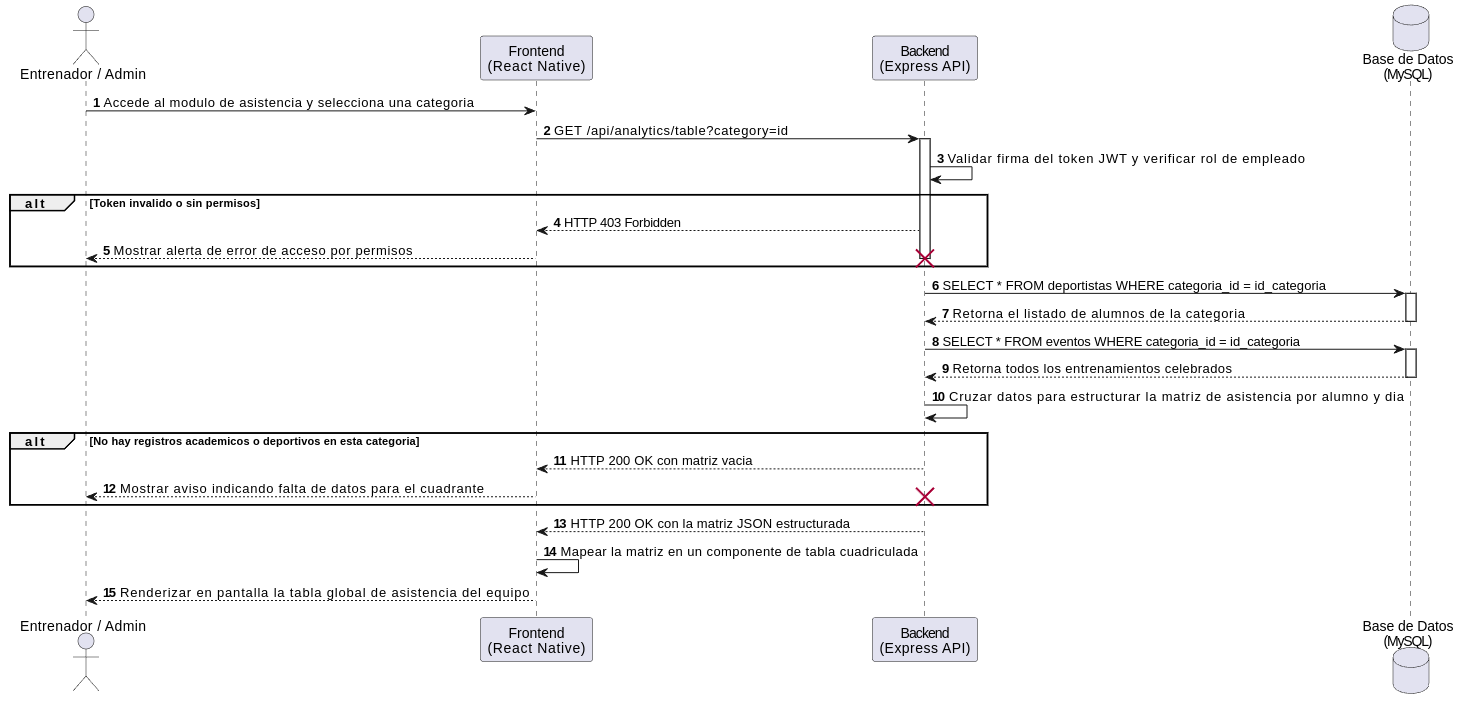
\includegraphics[width=0.9\textwidth]{diagramas/CU_15.drawio.png}
            \caption{Diagrama de secuencia del CU\_15.}
            \label{fig:seq_cu_15}
        \end{figure}

        \newpage
        \subsubsection{Módulo de control multimedia.}
        Este módulo gestiona el almacenamiento, asociación y visualización de recursos multimedia.

        \begin{figure}[htbp]
            \centering
            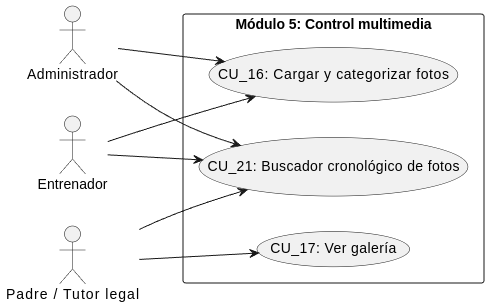
\includegraphics[width=0.8\textwidth]{diagramas/ControlMultimedia.drawio.png}
            \caption{Diagrama de control multimedia.}
            \label{fig:diagrama_control_multimedia}
        \end{figure}

        \clearpage
        \begin{table}[htbp]
        \centering
        \scriptsize
        \renewcommand{\arraystretch}{0.75}
        \begin{tabularx}{\textwidth}{|l|X|}
        \hline
        \rowcolor[HTML]{EFEFEF} 
        \textbf{Caso de Uso} & \textbf{Cargar y categorizar fotos (CU\_16)} \\ \hline
        \textbf{Actores} & Entrenador y Administrador. \\ \hline
        \textbf{Tipo} & Primario y esencial. \\ \hline
        \textbf{Referencias} & RF3.1, RF3.2, RF3.3 \\ \hline
        \textbf{Precondición} & El entrenador ha iniciado sesión y la app tiene permisos de cámara/galería. \\ \hline
        \textbf{Postcondición} & El archivo se almacena físicamente y sus metadatos quedan guardados en MySQL. \\ \hline
        \textbf{Propósito} & Permitir subir imágenes de los entrenamientos y clasificarlas según categoría técnica o carácter general. \\ \hline
        \textbf{Resumen} & El entrenador selecciona una foto de su dispositivo, elige la categoría técnica y el alumno, y confirma. El sistema almacena el archivo y guarda la vinculación en la base de datos. \\ \hline
        \textbf{Curso Normal} & 
        \textbf{1.} El Actor accede a la galería del entrenamiento y pulsa en ``Subir Imagen''.\newline
        \textbf{2.} El sistema abre el selector de archivos nativo del dispositivo.\newline
        \textbf{3.} El Actor selecciona la fotografía de su almacenamiento local.\newline
        \textbf{4.} El sistema muestra la previsualización de la imagen.\newline
        \textbf{5.} El Actor pulsa en ``Subir Foto''.\newline
        \textbf{6.} El backend procesa el archivo, lo guarda en el servidor físico y genera la URL pública.\newline
        \textbf{7.} El sistema inserta los metadatos y la URL en la tabla \textit{fotografías} de la base de datos.\newline
        \textbf{8.} El sistema refresca la interfaz del móvil confirmando la subida exitosa. \\ \hline
        \textbf{Cursos Alternos} & 
        \textbf{6a:} Archivo no válido o supera el tamaño máximo: el sistema interrumpe el proceso y muestra una alerta de error. \\ \hline
        \end{tabularx}
        \caption{Ficha caso de uso CU\_16.}
        \label{tab:cu_16}
        \end{table}

        \begin{figure}[htbp]
            \centering
            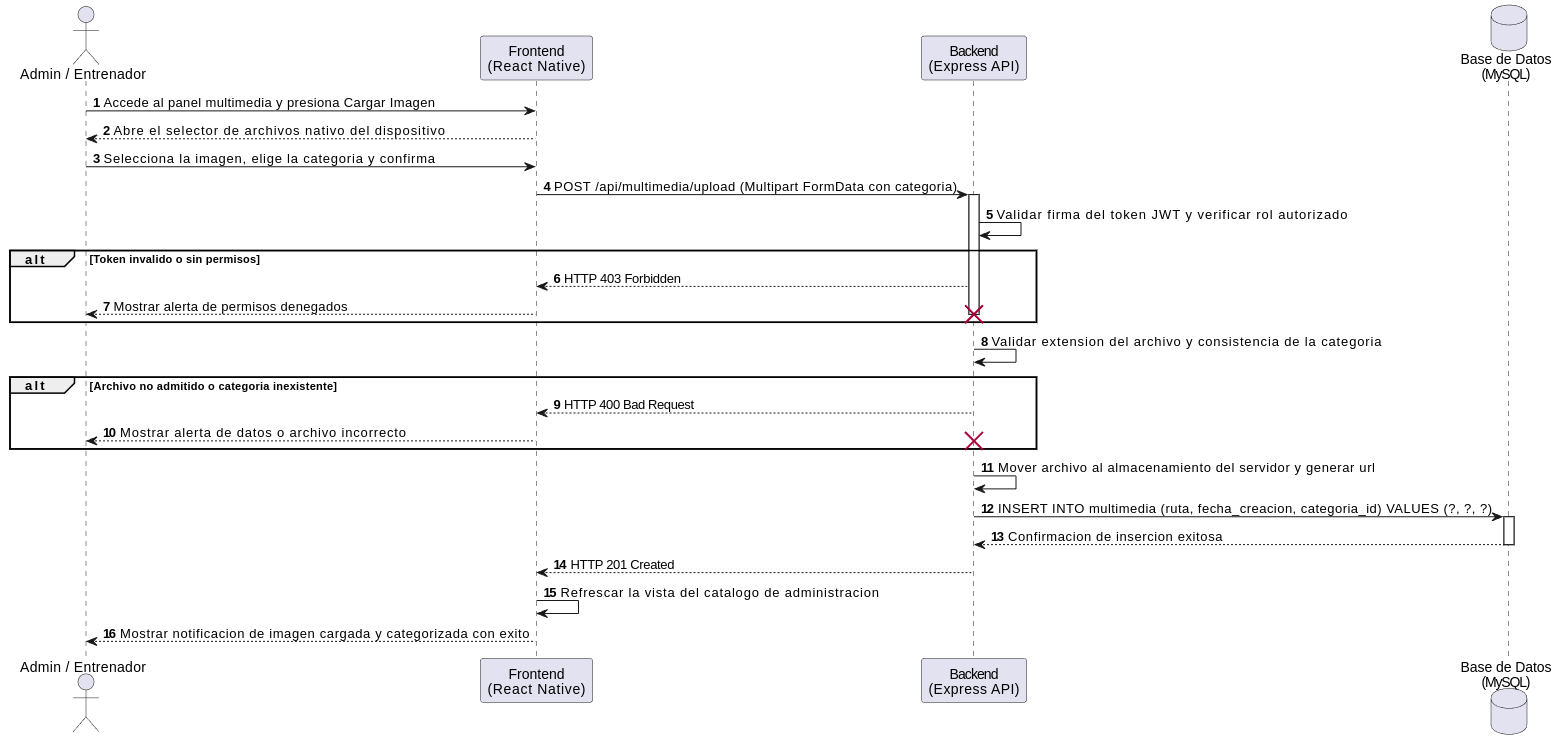
\includegraphics[width=0.9\textwidth]{diagramas/CU_16.drawio.png}
            \caption{Diagrama de secuencia del CU\_16.}
            \label{fig:seq_cu_16}
        \end{figure}

        \begin{table}[htbp]
        \centering
        \footnotesize
        \renewcommand{\arraystretch}{0.90}
        \begin{tabularx}{\textwidth}{|l|X|}
        \hline
        \rowcolor[HTML]{EFEFEF} 
        \textbf{Caso de Uso} & \textbf{Consultar galería de fotos (CU\_17)} \\ \hline
        \textbf{Actores} & Padre/Tutor legal \\ \hline
        \textbf{Tipo} & Primario y esencial. \\ \hline
        \textbf{Referencias} & RF3.3, RF3.4 \\ \hline
        \textbf{Precondición} & El padre ha iniciado sesión en la aplicación móvil y el entrenador ha subido fotos en la categoría del deportista. \\ \hline
        \textbf{Postcondición} & El sistema renderiza la cuadrícula de imágenes multimedia en la interfaz del usuario. \\ \hline
        \textbf{Propósito} & Permitir a los padres acceder a la galería multimedia. \\ \hline
        \textbf{Resumen} & El padre abre el apartado multimedia de su hijo. El sistema extrae la identidad del menor a través del token, consulta las URLs en la base de datos y renderiza la galería fotográfica clasificada en la pantalla del móvil. \\ \hline
        \textbf{Curso Normal} & 
        \textbf{1.} El Padre accede al menú ``Galería'' de su hijo en la aplicación móvil.\newline
        \textbf{2.} El sistema identifica el ID del deportista seleccionado y solicita al backend el listado de sus fotos.\newline
        \textbf{3.} El Padre filtra la búsqueda seleccionando una ``Categoría''.\newline
        \textbf{4.} El backend en Node.js consulta en MySQL la tabla \textit{fotografias} filtrando por el ID del deportista y la categoría técnica elegida.\newline
        \textbf{5.} El sistema devuelve el conjunto de metadatos y las URLs públicas de los archivos.\newline
        \textbf{6.} La aplicación móvil procesa las URLs y renderiza en pantalla una cuadrícula con las vistas en miniatura de las fotos. \\ \hline
        \textbf{Cursos Alternos} & 
        \textbf{4a:} El sistema comprueba que no existen fotos subidas o etiquetadas para ese alumno en la base de datos y muestra la pantalla vacía con el texto: ``Aún no hay fotografías disponibles para este deportista''. \\ \hline
        \end{tabularx}
        \caption{Ficha caso de uso CU\_17.}
        \label{tab:cu_17}
        \end{table}

        \begin{figure}[htbp]
            \centering
            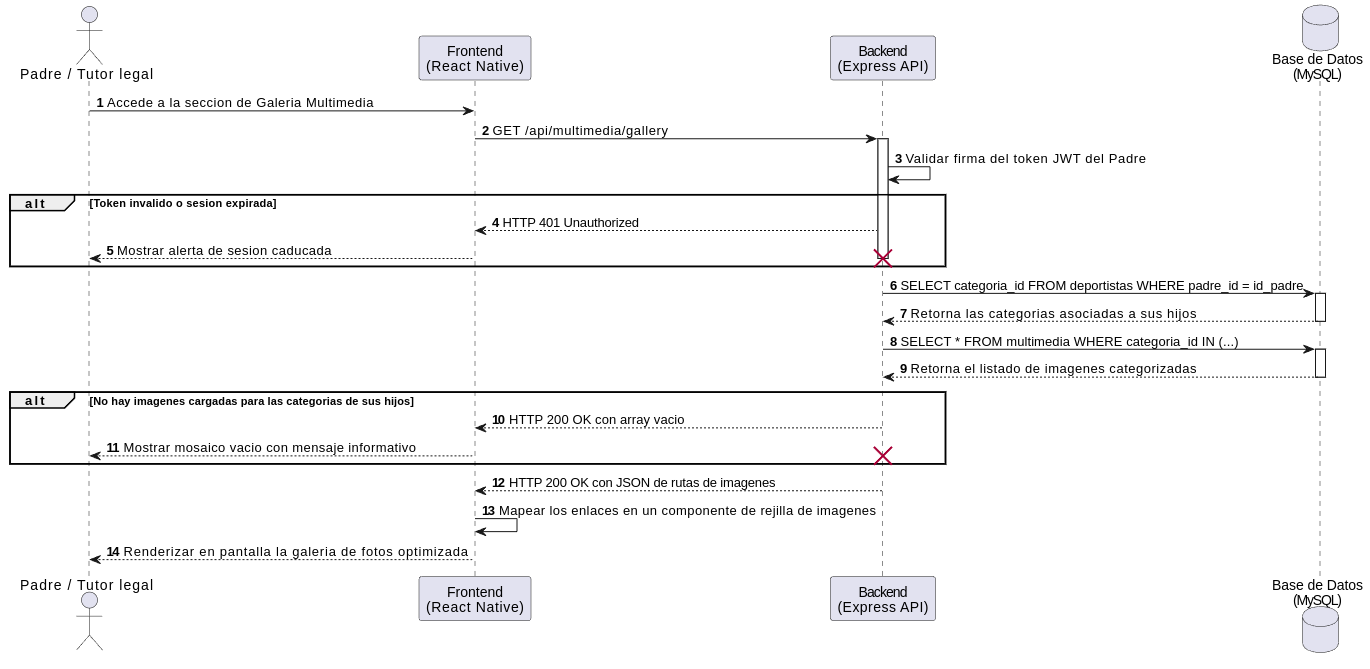
\includegraphics[width=0.9\textwidth]{diagramas/CU_17.drawio.png}
            \caption{Diagrama de secuencia del CU\_17.}
            \label{fig:seq_cu_17}
        \end{figure}

        \nopagebreak
        \begingroup
        \centering
        \footnotesize
        \renewcommand{\arraystretch}{0.95}
        \noindent\begin{tabularx}{\textwidth}{|l|X|}
        \hline
        \rowcolor[HTML]{EFEFEF} 
        \textbf{Caso de Uso} & \textbf{Buscar fotografías de forma cronológica (CU\_21)} \\ \hline
        \textbf{Actores} & General (Padre/Tutor legal, Entrenador y Administrador). \\ \hline
        \textbf{Tipo} & Primario y esencial. \\ \hline
        \textbf{Referencias} & RF3.3 \\ \hline
        \textbf{Precondición} & El usuario ha iniciado sesión y se encuentra dentro de la sección de galería multimedia de la aplicación. \\ \hline
        \textbf{Postcondición} & El sistema refresca la pantalla mostrando únicamente las imágenes que coinciden con el año y mes seleccionados. \\ \hline
        \textbf{Propósito} & Permitir a los usuarios localizar rápidamente el material gráfico de los entrenamientos filtrando la galería por criterios temporales (año y mes). \\ \hline
        \textbf{Resumen} & El usuario interactúa con el selector de fecha dentro de la galería multimedia. El sistema envía los parámetros de filtrado al backend, realiza la consulta indexada en MySQL y renderiza la nueva cuadrícula de imágenes en React Native. \\ \hline
        \textbf{Curso Normal} & 
        \textbf{1.} El Usuario accede al módulo de galería multimedia en la aplicación móvil.\newline
        \textbf{2.} El sistema habilita el componente de búsqueda cronológica.\newline
        \textbf{3.} El Usuario introduce un año y/o un mes específicos y pulsa el botón de filtrar.\newline
        \textbf{4.} El backend recibe los parámetros y realiza una consulta filtrada en la tabla \textit{fotografías} de MySQL.\newline
        \textbf{5.} El sistema devuelve el JSON con las URLs de las imágenes que cumplen el criterio.\newline
        \textbf{6.} El frontend descarga las referencias, actualiza el estado local y renderiza en React Native la cuadrícula con los resultados filtrados. \\ \hline
        \textbf{Cursos Alternos} & 
        \textbf{5a:} El backend ejecuta la consulta y consta que no hay imágenes almacenadas en el periodo indicado. Devuelve una respuesta vacía y la aplicación muestra en pantalla el texto informativo: ``No se han encontrado fotografías en el periodo seleccionado''. \\ \hline
        \end{tabularx}
        \captionof{table}{Ficha caso de uso CU\_21.}
        \label{tab:cu_21}
        \endgroup

        \newpage
        \section{Diseño}
        Tras el análisis recogido en la sección anterior, este apartado describe el diseño lógico de la aplicación móvil de gestión deportiva ---arquitectura, modelo de datos e interfaz---. En primer lugar se presenta la arquitectura por componentes; a continuación, el modelo de datos que sustenta usuarios, entrenamientos, asistencias y recursos multimedia; por último, se ilustran las pantallas principales mediante capturas de la aplicación desarrollada.

        \subsection{Arquitectura del sistema}
        \subsubsection{Visión general}
        La plataforma se despliega como una aplicación móvil nativa en la que el usuario accede a una interfaz interactiva desarrollada en React Native. El cliente se comunica con un servidor backend mediante una API REST; la lógica de negocio y la persistencia residen en este servidor, que almacena la información en una base de datos relacional MySQL. En lugar de repartir la funcionalidad en microservicios independientes, el backend se implementa como un monolito modular: un único proceso desplegable organizado en módulos de dominio (autenticación, gestión de entrenamientos, control de asistencia y almacenamiento multimedia). Esta organización reduce la complejidad operativa del TFG y mantiene un acoplamiento acotado entre áreas funcionales.

        La figura \ref{fig:arq_skiclubmanager} resume la arquitectura general del sistema. Además de la interacción cliente--servidor--base de datos, el cliente gestiona de forma local el estado de la sesión mediante la Context API de React Native, asegurando la persistencia del token JWT para las peticiones autenticadas, mientras que el módulo de rendimiento transforma los históricos de asistencia en componentes visuales mediante la librería gráfica del frontend.

        \begin{figure}[htbp]
            \centering
            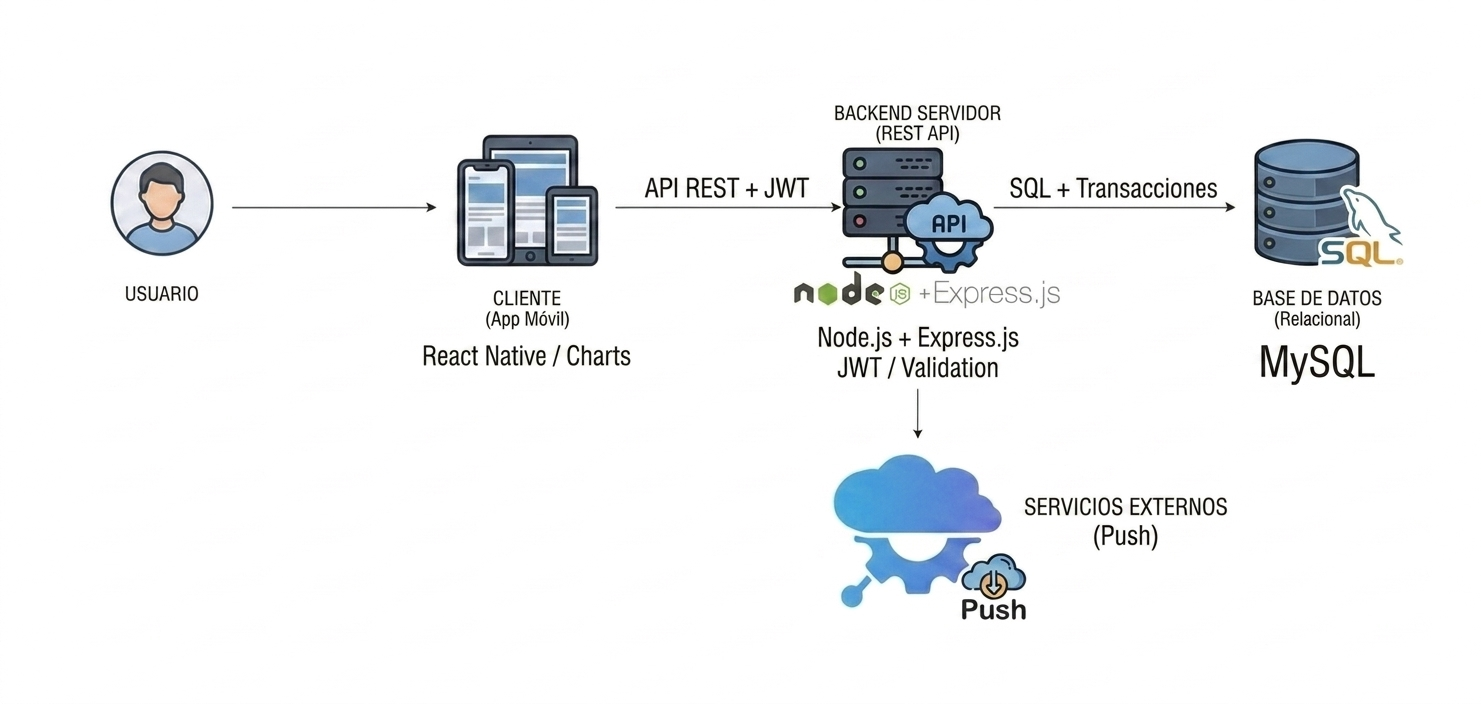
\includegraphics[width=0.9\textwidth]{imagenes/arquitectura.png}
            \caption{Arquitectura de SkiClubManager.}
            \label{fig:arq_skiclubmanager}
        \end{figure}

        \subsubsection{Componentes del backend}

        El servidor de la plataforma se organiza como un monolito modular. Cada módulo de dominio agrupa el controlador REST que expone los endpoints, el servicio donde reside la lógica de negocio y, cuando corresponde, las entidades de persistencia asociadas a la base de datos MySQL. Todos los módulos comparten la misma base de datos relacional. Esta organización mantiene un reparto claro de responsabilidades sin fragmentar el despliegue en varios servicios independientes.

        El conjunto completo de rutas que componen la API REST del sistema se detalla y referencia dinámicamente a través de la \ref{tab:endpoints_backend_1}, la \ref{tab:endpoints_backend_2}, la \ref{tab:endpoints_eventos} y la la \ref{tab:endpoints_gestion}.

        \begin{table}[htbp]
        \centering
        \footnotesize
        \renewcommand{\arraystretch}{1.1}
        \begin{tabularx}{\textwidth}{|l|l|l|X|}
        \hline
        \rowcolor[HTML]{EFEFEF} 
        \textbf{Fichero de Ruta} & \textbf{Verbo} & \textbf{Endpoint} & \textbf{Propósito y Lógica de Negocio} \\ \hline
        autorizacion.js & POST & /login & Autenticación de credenciales y firma de tokens JWT. \\ \hline
        autorizacion.js & POST & /solicitar-registro & Gestión de alta en la plataforma para nuevos usuarios. \\ \hline
        autorizacion.js & POST & /forgot-password & Solicitud de recuperación de contraseña por email. \\ \hline
        autorizacion.js & POST & /reset-password & Configuración de la nueva credencial del usuario. \\ \hline
        autorizacion.js & POST & /change-password & Actualización de contraseña desde el perfil activo. \\ \hline
        autorizacion.js & POST & /refresh & Renovación automática de un accessToken mediante el refresh token. \\ \hline
        usuarios.js & GET & / & Obtención del listado global de usuarios del sistema (Admin). \\ \hline
        usuarios.js & GET & /yo & Recuperación del perfil del usuario autenticado en sesión. \\ \hline
        usuarios.js & GET & /:id & Consulta de un perfil de usuario específico por su identificador. \\ \hline
        usuarios.js & POST & / & Registro directo de una nueva entidad de usuario. \\ \hline
        \end{tabularx}
        \caption{Endpoints REST de la API: Control de Autorización y Gestión de Usuarios.}
        \label{tab:endpoints_backend_1}
        \end{table}

        \begin{table}[htbp]
        \centering
        \footnotesize
        \renewcommand{\arraystretch}{1.1}
        \begin{tabularx}{\textwidth}{|l|l|l|X|}
        \hline
        \rowcolor[HTML]{EFEFEF} 
        \textbf{Fichero de Ruta} & \textbf{Verbo} & \textbf{Endpoint} & \textbf{Propósito y Lógica de Negocio} \\ \hline
        deportista.js & GET & /mis\_hijos & Listado de los esquiadores vinculados al tutor legal (Padre). \\ \hline
        deportista.js & POST & /anadir\_hijo & Alta e inserción relacional de un nuevo hijo en MySQL. \\ \hline
        deportista.js & GET & /expedientes-completos & Consulta agregada de deportistas y sus tutores asignados. \\ \hline
        deportista.js & PUT & /actualizar/:id & Modificación de los datos del expediente técnico de un esquiador. \\ \hline
        deportista.js & DELETE & /eliminar/:id & Borrado físico de un deportista de la base de datos por su ID. \\ \hline
        entrenadores.js & POST & / & Registro e inicialización de un nuevo perfil de entrenador. \\ \hline
        entrenadores.js & GET & / & Recuperación del listado general del personal técnico del club. \\ \hline
        entrenadores.js & GET & /mi\_perfil & Consulta del perfil privado y categoría del entrenador en sesión. \\ \hline
        entrenadores.js & GET & /:id & Búsqueda parametrizada de un entrenador específico. \\ \hline
        entrenadores.js & PUT & /:id & Actualización de los datos laborales o de contacto del técnico. \\ \hline
        entrenadores.js & DELETE & /:id & Baja del sistema de la ficha de un entrenador específico. \\ \hline
        \end{tabularx}
        \caption{Endpoints REST de la API: Fichas de Deportistas y Personal de Entrenadores.}
        \label{tab:endpoints_backend_2}
        \end{table}

        \begin{table}[htbp]
        \centering
        \scriptsize
        \renewcommand{\arraystretch}{0.95}
        \begin{tabularx}{\textwidth}{|l|l|l|X|}
        \hline
        \rowcolor[HTML]{EFEFEF} 
        \textbf{Fichero de Ruta} & \textbf{Verbo} & \textbf{Endpoint} & \textbf{Propósito y Lógica de Negocio} \\ \hline
        \texttt{eventos.js} & POST & \texttt{/} & Creación de un entrenamiento o competición deportiva. \\ \hline
        \texttt{eventos.js} & GET & \texttt{/todos} & Recuperación de todo el calendario histórico y futuro del club. \\ \hline
        \texttt{eventos.js} & GET & \texttt{/filtrados} & Eventos segmentados por categorías del usuario identificado. \\ \hline
        \texttt{eventos.js} & GET & \texttt{/entrenador/mios} & Entrenamientos vinculados a la categoría específica del técnico. \\ \hline
        \texttt{eventos.js} & GET & \texttt{/entrenador/asistencias} & Panel de control de faltas y asistencias para el entrenador. \\ \hline
        \texttt{eventos.js} & GET & \texttt{/padre/asistencias} & Histórico de asistencia de los hijos para control del tutor. \\ \hline
        \texttt{eventos.js} & GET & \texttt{/apuntados} & Eventos en los que los deportistas ya han sido confirmados. \\ \hline
        \texttt{eventos.js} & GET & \texttt{/admin/asistencias} & Auditoría completa de asistencia a nivel de administración. \\ \hline
        \texttt{eventos.js} & GET & \texttt{/viaje/:viajeId/pasajeros} & Listado de deportistas con plaza asignada en un trayecto. \\ \hline
        \texttt{eventos.js} & GET & \texttt{/padre/evento/:id} & Detalle extendido de un evento enfocado al rol de los padres. \\ \hline
        \texttt{eventos.js} & GET & \texttt{/:id/inscritos} & Retorna los alumnos que asistirán a un entrenamiento concreto. \\ \hline
        \texttt{eventos.js} & GET & \texttt{/:id/apuntado} & Validación de la inscripción previa de un deportista. \\ \hline
        \texttt{eventos.js} & POST & \texttt{/:id/apuntar} & Inscripción activa de un deportista en una sesión de pista. \\ \hline
        \texttt{eventos.js} & DELETE & \texttt{/:id/desapuntar} & Cancelación de la asistencia de un deportista a un evento. \\ \hline
        \texttt{eventos.js} & PUT & \texttt{/:id/transporte-hijo} & Modificación del método de subida asignado al menor. \\ \hline
        \texttt{eventos.js} & PUT & \texttt{/:id} & Edición de parámetros (tipo de nieve, disciplina) de un evento. \\ \hline
        \texttt{eventos.js} & DELETE & \texttt{/:id} & Eliminación del registro de un entrenamiento del calendario. \\ \hline
        \end{tabularx}
        \caption{Endpoints REST de la API: Gestión y Planificación de Eventos.}
        \label{tab:endpoints_eventos}
        \end{table}

        \begin{table}[htbp]
        \centering
        \scriptsize
        \renewcommand{\arraystretch}{0.95}
        \begin{tabularx}{\textwidth}{|l|l|l|X|}
        \hline
        \rowcolor[HTML]{EFEFEF} 
        \textbf{Fichero de Ruta} & \textbf{Verbo} & \textbf{Endpoint} & \textbf{Propósito y Lógica de Negocio} \\ \hline
        \texttt{fotos.js} & GET & \texttt{/} & Consulta indexada de las capturas multimedia de los entrenamientos. \\ \hline
        \texttt{fotos.js} & POST & \texttt{/} & Almacenamiento físico de una foto de pista y registro de su URL. \\ \hline
        \texttt{fotos.js} & DELETE & \texttt{/ y /:id} & Eliminación masiva o individual de recursos multimedia. \\ \hline
        \texttt{solicitud.js} & GET & \texttt{/} & Listado de solicitudes de justificación administrativas pendientes. \\ \hline
        \texttt{solicitud.js} & POST & \texttt{/} & Envío de una nueva solicitud o justificante desde la aplicación. \\ \hline
        \texttt{solicitud.js} & POST & \texttt{/:id/aceptar} & Aprobación de una solicitud con impacto en el estado del alumno. \\ \hline
        \texttt{solicitud.js} & POST & \texttt{/:id/rechazar} & Desestimación o eliminación de una solicitud administrativa. \\ \hline
        \texttt{transporte.js} & POST & \texttt{/reservar} & Bloqueo de plazas de transporte corporativo para la subida. \\ \hline
        \texttt{transporte.js} & GET & \texttt{/entrenador} & Consulta de rutas planificadas para el personal de entrenadores. \\ \hline
        \texttt{transporte.js} & GET & \texttt{/:id/pasajeros} & Control de la lista de pasajeros del bus técnico del club. \\ \hline
        \texttt{transporte.js} & GET & \texttt{/padre} & Visualización de las rutas disponibles para el rol de familia. \\ \hline
        \texttt{transporte.js} & GET & \texttt{/admin y /admin/:id/pasajeros} & Gestión e inspección analítica global de la logística de transporte. \\ \hline
        \end{tabularx}
        \caption{Endpoints REST de la API: Recursos Multimedia, Solicitudes Administrativas y Gestión Logística de Transporte.}
        \label{tab:endpoints_gestion}
        \end{table}

        \begin{figure}[htbp]
            \centering
            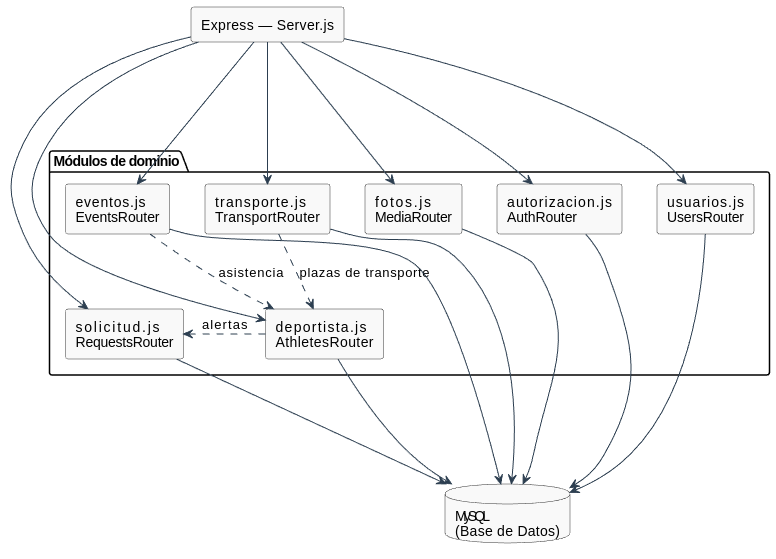
\includegraphics[width=0.9\textwidth]{diagramas/Arquitectura.drawio.png}
            \caption{Organización modular del servidor (backend).}
            \label{fig:org_modular_backend}
        \end{figure}

        \newpage
        \subsubsection{Componentes del frontend}

        La interfaz de usuario de la plataforma se ha desarrollado como una aplicación móvil nativa multiplataforma utilizando el entorno React Native y TypeScript. La navegación interna y el flujo de pantallas se gestionan mediante la librería React Navigation, implementando una estrategia de enrutamiento dinámico basado en el estado de autenticación y el rol asignado al usuario (Administrador, Entrenador o Padre). 

        El punto de entrada de la navegación se centraliza en el componente \texttt{StackNavigator.tsx}, el cual evalúa los parámetros \texttt{isAuthenticated} y \texttt{rol} provistos por el contexto global de seguridad (\texttt{AuthContext}). Si el usuario no está autenticado, el enrutador expone exclusivamente las pantallas del bloque común. Una vez validada la sesión mediante el token JWT, el sistema inyecta un sub-navegador específico (\texttt{AdminNavigator}, \texttt{EntrenadorNavigator} o \texttt{PadreNavigator}) que combina estructuras de navegación por pestañas (\texttt{Tabs}) y pilas de pantallas (\texttt{Stack}).

        Las pantallas que componen los diferentes módulos de la aplicación móvil se detallan e indexan en la \ref{tab:frontend_screens_1} y en la \ref{tab:frontend_screens_2}.

        \begin{table}[htbp]
        \centering
        \scriptsize
        \renewcommand{\arraystretch}{0.95}
        \begin{tabularx}{\textwidth}{|l|l|X|}
        \hline
        \rowcolor[HTML]{EFEFEF} 
        \textbf{Bloque / Carpeta} & \textbf{Fichero de Pantalla} & \textbf{Funcionalidad e Interfaz de Usuario} \\ \hline
        \texttt{comun/} & \texttt{LoginScreen.tsx} & Formulario de acceso al sistema con validación de credenciales. \\ \hline
        \texttt{comun/} & \texttt{ForgotPassword.tsx} & Interfaz para la solicitud de recuperación de credenciales por correo. \\ \hline
        \texttt{comun/} & \texttt{CambiarContrasena.tsx} & Formulario seguro para la actualización de la contraseña del usuario. \\ \hline
        \texttt{padre/} & \texttt{RegisterRequestScreen.tsx} & Formulario de alta inicial y pre-registro para tutores legales. \\ \hline
        \texttt{padre/} & \texttt{HomePadre.tsx} & Panel principal de familias con accesos directos y notificaciones. \\ \hline
        \texttt{padre/} & \texttt{AnadirHijo.tsx} & Formulario para vincular y registrar un esquiador menor bajo su tutela. \\ \hline
        \texttt{padre/} & \texttt{CalendarioPadre.tsx} & Visualización del calendario técnico y eventos de entrenamiento. \\ \hline
        \texttt{padre/} & \texttt{DetalleEventoPadreApuntar.tsx} & Vista extendida de eventos con opción de inscripción para sus hijos. \\ \hline
        \texttt{padre/} & \texttt{DetalleEventoPadreDesapuntar.tsx} & Cancelación de inscripciones previas y gestión de bajas del entrenamiento. \\ \hline
        \texttt{padre/} & \texttt{AsistenciaHijoPista.tsx} & Consulta analítica del histórico de faltas y presencias en nieve de los hijos. \\ \hline
        \texttt{padre/} & \texttt{AsistenciaTransporte.tsx} & Estado y reserva de plazas en los vehículos de subida a la estación. \\ \hline
        \texttt{padre/} & \texttt{GaleriaPadre.tsx} & Muro multimedia cronológico para visualizar fotos técnicas de su hijo. \\ \hline
        \texttt{padre/} & \texttt{PerfilPadre.tsx} & Visualización de los datos del tutor legal y ajustes de la cuenta. \\ \hline
        \texttt{padre/} & \texttt{GestionarPerfil.tsx} & Formulario de edición de información personal y de contacto de la familia. \\ \hline
        \end{tabularx}
        \caption{Componentes del Frontend: Pantallas del Bloque Común y del Rol del Padre.}
        \label{tab:frontend_screens_1}
        \end{table}

        \begin{table}[htbp]
        \centering
        \scriptsize
        \renewcommand{\arraystretch}{0.95}
        \begin{tabularx}{\textwidth}{|l|l|X|}
        \hline
        \rowcolor[HTML]{EFEFEF} 
        \textbf{Bloque / Carpeta} & \textbf{Fichero de Pantalla} & \textbf{Funcionalidad e Interfaz de Usuario} \\ \hline
        \texttt{entrenador/} & \texttt{HomeEntrenador.tsx} & Panel operativo del técnico con resumen de entrenamientos del día. \\ \hline
        \texttt{entrenador/} & \texttt{CalendarioEntrenador.tsx} & Agenda mensualizada de las sesiones y competiciones asignadas. \\ \hline
        \texttt{entrenador/} & \texttt{CrearEvento.tsx} & Formulario técnico para la planificación de nuevas sesiones en pista. \\ \hline
        \texttt{entrenador/} & \texttt{ModificarEntrenamiento.tsx} & Panel de edición de parámetros técnicos del entrenamiento guardado. \\ \hline
        \texttt{entrenador/} & \texttt{AsistenciaEntrenamiento.tsx} & Interfaz interactiva para el control de asistencia por grupos en nieve. \\ \hline
        \texttt{entrenador/} & \texttt{AsistenciaPista.tsx} & Consolidación y cierre del registro de faltas del día de esquí. \\ \hline
        \texttt{entrenador/} & \texttt{AdministrarTransporte.tsx} & Control y verificación de la ocupación del bus técnico del club. \\ \hline
        \texttt{entrenador/} & \texttt{GaleriaEntrenador.tsx} & Herramienta para capturar, asociar y subir material fotográfico. \\ \hline
        \texttt{entrenador/} & \texttt{PerfilEntrenador.tsx} & Información profesional, titulación y categorías asignadas al técnico. \\ \hline
        \texttt{admin/} & \texttt{HomeAdmin.tsx} & Cuadro de mando global del club con métricas y alertas del sistema. \\ \hline
        \texttt{admin/} & \texttt{AdministrarUsuarios.tsx} & Panel CRUD para la gestión y asignación de roles en la plataforma. \\ \hline
        \texttt{admin/} & \texttt{AdministrarEntrenador.tsx} & Alta, baja y control del personal técnico y directores de carrera. \\ \hline
        \texttt{admin/} & \texttt{ListaEntrenadores.tsx} & Visualización global e indexada del cuerpo técnico del club de esquí. \\ \hline
        \texttt{admin/} & \texttt{GestionarDeportistas.tsx} & Base de datos de expedientes, licencias y categorías de los corredores. \\ \hline
        \texttt{admin/} & \texttt{AdministrarTransporte.tsx} & Configuración logística de trayectos, conductores y plazas de subida. \\ \hline
        \texttt{admin/} & \texttt{GaleriaAdmin.tsx} & Moderación global de los recursos multimedia cargados en el servidor. \\ \hline
        \end{tabularx}
        \caption{Componentes del Frontend: Pantallas del Rol del Entrenador y del Rol del Administrador.}
        \label{tab:frontend_screens_2}
        \end{table}

        \begin{figure}[htbp]
            \centering
            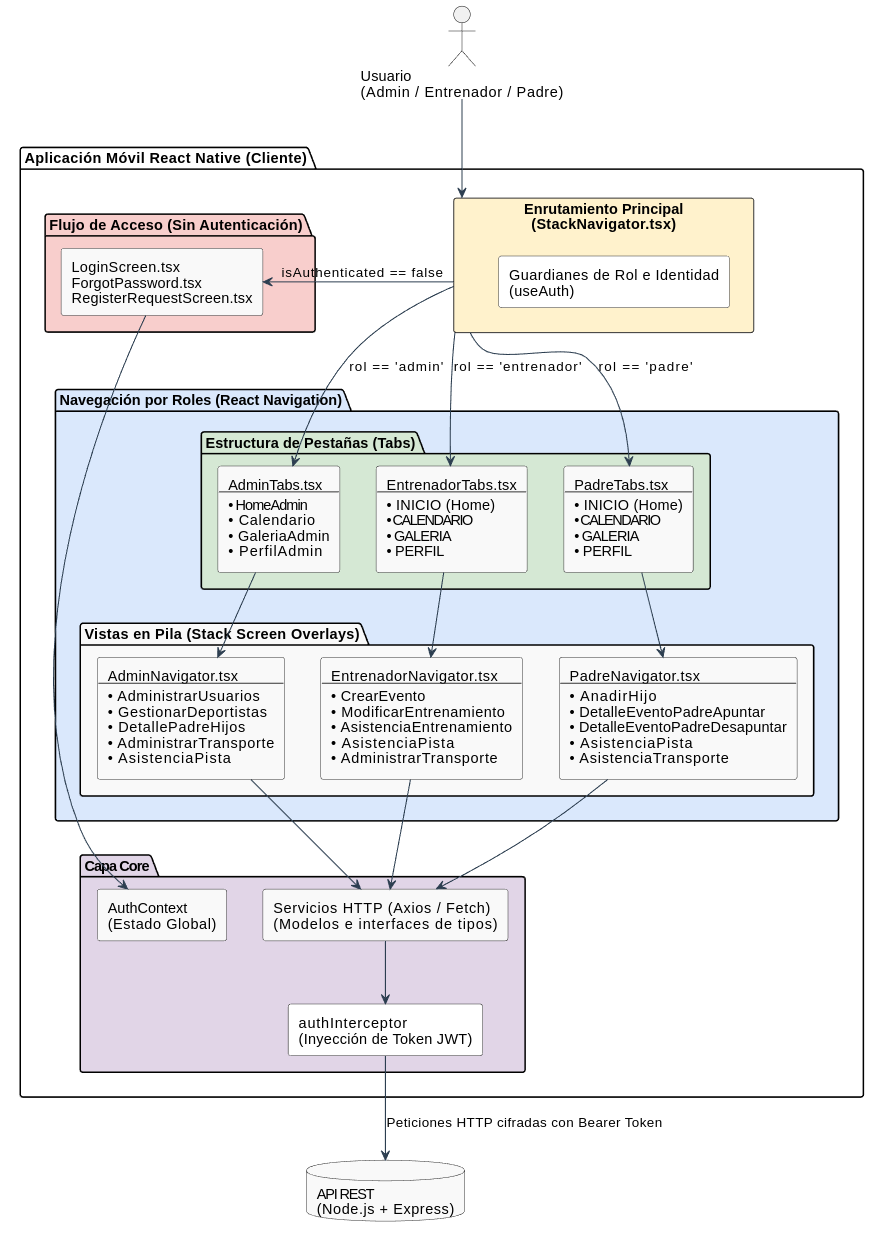
\includegraphics[width=0.95\textwidth]{diagramas/OrganizacionCliente.drawio.png}
            \caption{Arquitectura y enrutamiento dinámico de la aplicación móvil según el rol de usuario.}
            \label{fig:organizacion_cliente}
        \end{figure}

        \newpage
        \subsubsection{Modelo de datos}

        La plataforma persiste toda su información en una base de datos relacional gestionada a través de MySQL. El esquema lógico se define mediante un mapeo directo de entidad-tabla, aplicando restricciones de integridad referencial mediante claves foráneas, reglas de unicidad para evitar duplicidades en registros críticos (como credenciales o vinculaciones familiares) y relaciones muchos a muchos administradas mediante tablas de ruptura o pivote.

        El modelo de datos ha sido diseñado para responder de forma estricta a las necesidades operativas y de negocio de la plataforma, estructurándose en torno a los siguientes pilares funcionales:
        
        \begin{figure}[htbp]
            \centering
            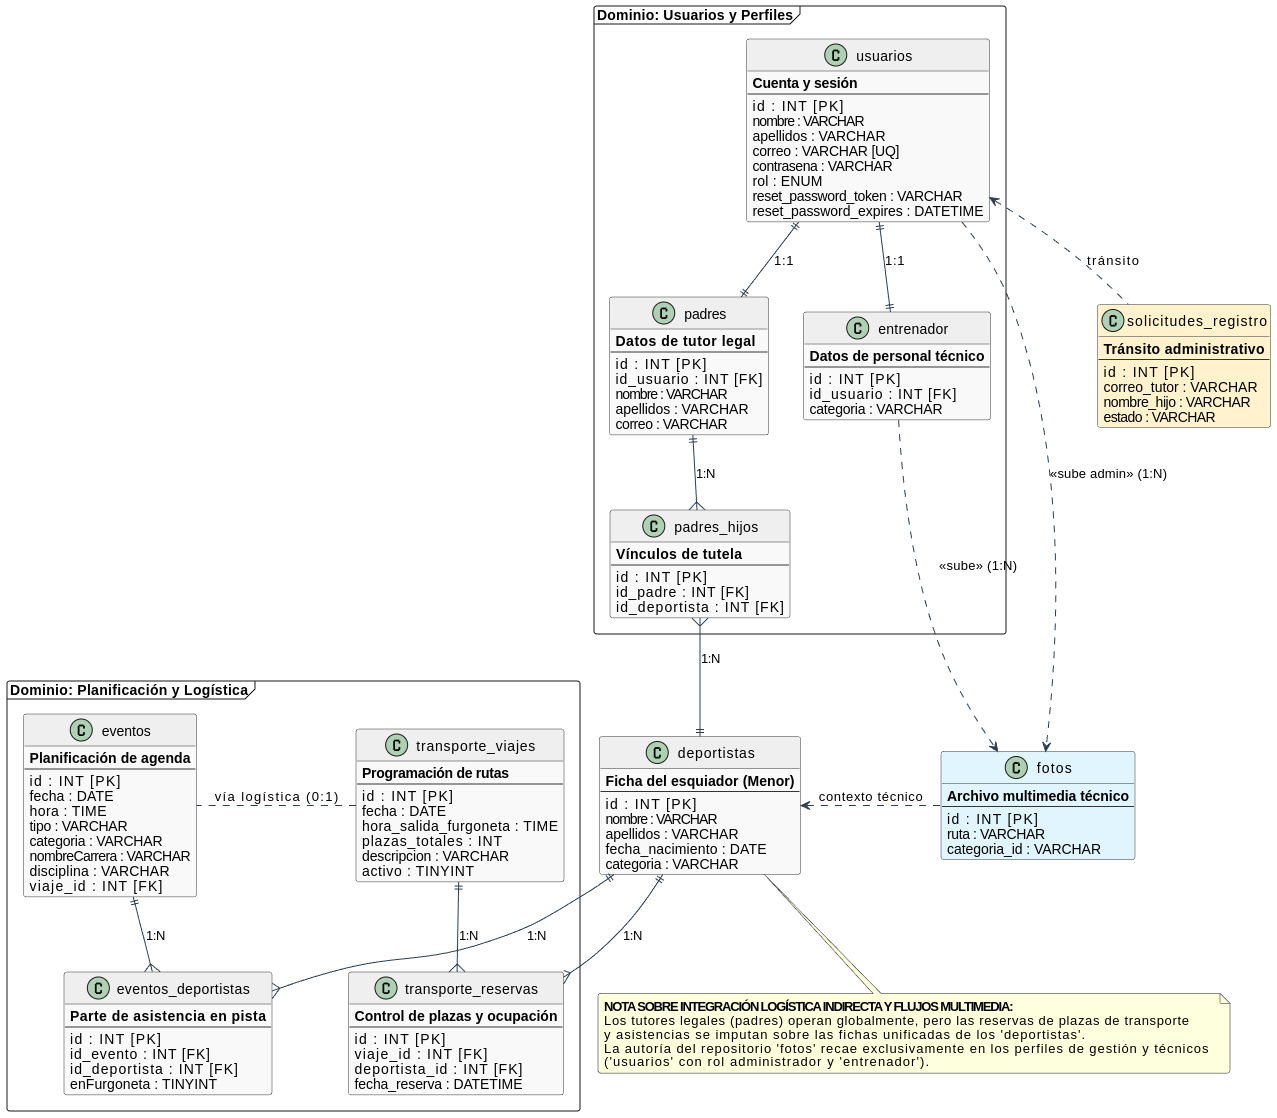
\includegraphics[width=1\textwidth]{diagramas/DiagramaBaseDatos.drawio.png}
            \caption{Diagrama del modelo relacional}
            \label{fig:relacional_usuarios_perfiles}
        \end{figure}

        \newpage
        \subsection{Usuarios y Perfiles}

        A continuación, se detallan de forma pormenorizada las tablas físicas que componen el dominio de gestión de usuarios, perfiles y filiaciones, especificando el tipo de dato, la clave y el propósito de cada atributo según la implementación real en el motor MySQL.

        \subsubsection{Tabla: usuarios}
        Esta entidad actúa como el núcleo del sistema de autenticación global de la plataforma, almacenando las credenciales de acceso y el rol asignado para la autorización en las aplicaciones.

        \begin{table}[htbp]
        \centering
        \scriptsize
        \renewcommand{\arraystretch}{1.0}
        \setlength{\tabcolsep}{4pt}
        \begin{tabularx}{\textwidth}{|l|l|l|X|}
        \hline
        \rowcolor[HTML]{EFEFEF} 
        \textbf{Campo} & \textbf{Tipo de Dato} & \textbf{Clave} & \textbf{Descripción y Restricciones} \\ \hline
        \texttt{id} & INT & PK (AI) & Identificador único auto-incremental de la cuenta. \\ \hline
        \texttt{nombre} & VARCHAR(255) & - & Nombre de pila del usuario registrado. \\ \hline
        \texttt{apellidos} & VARCHAR(255) & - & Apellidos completos del usuario. \\ \hline
        \texttt{correo} & VARCHAR(255) & UNIQUE & Correo electrónico utilizado como login (clave única). \\ \hline
        \texttt{fecha\_nacimiento} & DATE & - & Fecha de nacimiento del usuario de la cuenta. \\ \hline
        \texttt{contrasena} & VARCHAR(255) & - & Hash seguro de la clave de acceso cifrada. \\ \hline
        \texttt{rol} & ENUM(...) & - & Perfil del sistema: \texttt{'admin'}, \texttt{'entrenador'}, \texttt{'padre'}. \\ \hline
        \texttt{reset\_password\_token} & VARCHAR(255) & - & Token temporal para el flujo de recuperación de contraseña. \\ \hline
        \texttt{reset\_password\_expires} & DATETIME & - & Fecha de expiración de la validez del token de reinicio. \\ \hline
        \end{tabularx}
        \caption{Especificación física de la tabla \texttt{usuarios}.}
        \label{tab:dic_usuarios}
        \end{table}

        \subsubsection{Tabla: padres}
        Extiende la información de la cuenta base para aquellos usuarios que operan con el rol de tutores legales de los esquiadores.

        \begin{table}[htbp]
        \centering
        \scriptsize
        \renewcommand{\arraystretch}{1.0}
        \setlength{\tabcolsep}{4pt}
        \begin{tabularx}{\textwidth}{|l|l|l|X|}
        \hline
        \rowcolor[HTML]{EFEFEF} 
        \textbf{Campo} & \textbf{Tipo de Dato} & \textbf{Clave} & \textbf{Descripción y Restricciones} \\ \hline
        \texttt{id} & INT & PK (AI) & Identificador único del perfil del padre/tutor. \\ \hline
        \texttt{id\_usuario} & INT & FK & Referencia al identificador base en la tabla \texttt{usuarios}. \\ \hline
        \texttt{nombre} & VARCHAR(255) & - & Nombre del tutor legal. \\ \hline
        \texttt{apellidos} & VARCHAR(255) & - & Apellidos del tutor legal. \\ \hline
        \texttt{correo} & VARCHAR(255) & - & Correo electrónico de contacto o notificaciones. \\ \hline
        \end{tabularx}
        \caption{Especificación física de la tabla \texttt{padres}.}
        \label{tab:dic_padres}
        \end{table}
        \newpage

        \subsubsection{Tabla: entrenador}
        Almacena la especialización del perfil técnico del club, acotando el ámbito deportivo del profesional.

        \begin{table}[htbp]
        \centering
        \scriptsize
        \renewcommand{\arraystretch}{1.0}
        \setlength{\tabcolsep}{4pt}
        \begin{tabularx}{\textwidth}{|l|l|l|X|}
        \hline
        \rowcolor[HTML]{EFEFEF} 
        \textbf{Campo} & \textbf{Tipo de Dato} & \textbf{Clave} & \textbf{Descripción y Restricciones} \\ \hline
        \texttt{id} & INT & PK (AI) & Identificador único del perfil del entrenador. \\ \hline
        \texttt{categoria} & VARCHAR(100) & - & Grupo o categoría alpina asignada (ej. U14, U16, Tec.). \\ \hline
        \end{tabularx}
        \caption{Especificación física de la tabla \texttt{entrenador}.}
        \label{tab:dic_entrenador}
        \end{table}

        \subsubsection{Tabla: deportistas}
        Fichas y expedientes deportivos de los atletas del club de esquí. Al ser menores, dependen relacionalmente de sus tutores.

        \begin{table}[htbp]
        \centering
        \scriptsize
        \renewcommand{\arraystretch}{1.0}
        \setlength{\tabcolsep}{4pt}
        \begin{tabularx}{\textwidth}{|l|l|l|X|}
        \hline
        \rowcolor[HTML]{EFEFEF} 
        \textbf{Campo} & \textbf{Tipo de Dato} & \textbf{Clave} & \textbf{Descripción y Restricciones} \\ \hline
        \texttt{id} & INT & PK (AI) & Identificador único del esquiador. \\ \hline
        \texttt{nombre} & VARCHAR(255) & - & Nombre del deportista menor de edad. \\ \hline
        \texttt{apellidos} & VARCHAR(255) & - & Apellidos del deportista. \\ \hline
        \texttt{fecha\_nacimiento} & DATE & - & Fecha de nacimiento del atleta (determina su categoría por edad). \\ \hline
        \texttt{categoria} & VARCHAR(100) & - & Categoría de competición alpina asignada. \\ \hline
        \end{tabularx}
        \caption{Especificación física de la tabla \texttt{deportistas}.}
        \label{tab:dic_deportistas}
        \end{table}

        \subsubsection{Tabla: padres\_hijos}
        Tabla relacional de ruptura muchos a muchos ($M:N$) encargada de coordinar la patria potestad y los lazos de parentesco del club.

        \begin{table}[htbp]
        \centering
        \scriptsize
        \renewcommand{\arraystretch}{1.0}
        \setlength{\tabcolsep}{4pt}
        \begin{tabularx}{\textwidth}{|l|l|l|X|}
        \hline
        \rowcolor[HTML]{EFEFEF} 
        \textbf{Campo} & \textbf{Tipo de Dato} & \textbf{Clave} & \textbf{Descripción y Restricciones} \\ \hline
        \texttt{id} & INT & PK (AI) & Identificador correlativo del vínculo. \\ \hline
        \texttt{id\_padre} & INT & FK & Clave foránea orientada al registro de la tabla \texttt{padres}. \\ \hline
        \texttt{id\_deportista} & INT & FK & Clave foránea orientada al registro de la tabla \texttt{deportistas}. \\ \hline
        \end{tabularx}
        \caption{Especificación física de la tabla intermedia \texttt{padres\_hijos}.}
        \label{tab:dic_padres_hijos}
        \end{table}

        La estructura física, las restricciones de integridad y la tipificación de datos que gobiernan este dominio se ilustran de forma detallada en el diagrama del modelo relacional de la \ref{fig:relacional_usuarios_perfiles}.

        \begin{figure}[htbp]
            \centering
            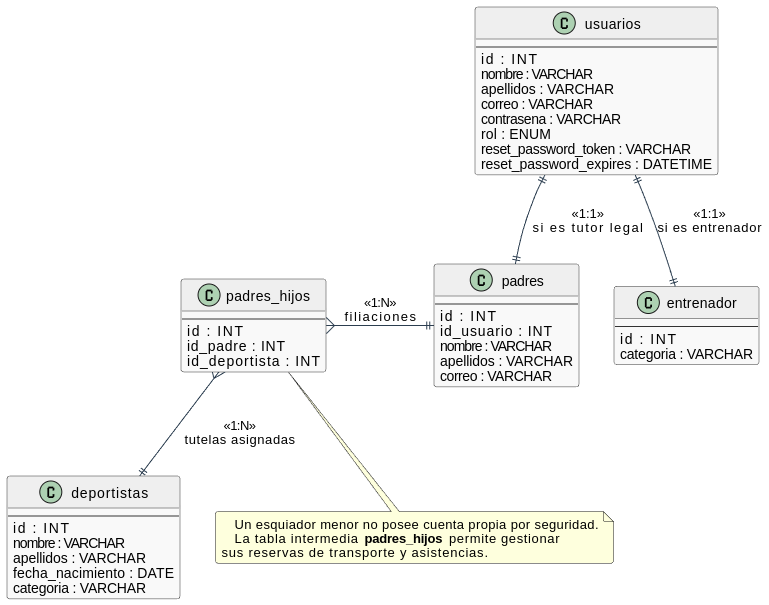
\includegraphics[width=0.75\textwidth]{diagramas/DiagramaModeloUsuario.drawio.png}
            \caption{Modelo relacional de datos Usuarios y Perfiles.}
            \label{fig:relacional_usuarios_perfiles}
        \end{figure}

        \newpage

        \subsection{Entrenamientos y Asistencias}

        Este bloque del modelo de datos gestiona la planificación del calendario del club y el seguimiento operativo del rendimiento físico y la asistencia en las pistas de esquí. Estas tablas operan para permitir la vinculación de las convocatorias de entrenamientos o carreras oficiales con la presencia real de los esquiadores, optimizando la posterior explotación estadística y visualización de progreso deportivo de los atletas.

        A continuación, se especifican las tablas físicas y las restricciones técnicas correspondientes a este bloque funcional del motor MySQL.

        \subsubsection{Tabla: eventos}
        Almacena las sesiones técnicas, entrenamientos físicos y competiciones del club programadas en el calendario deportivo.

        \begin{table}[htbp]
        \centering
        \scriptsize
        \renewcommand{\arraystretch}{0.9}
        \setlength{\tabcolsep}{4pt}
        \begin{tabularx}{\textwidth}{|l|l|l|X|}
        \hline
        \rowcolor[HTML]{EFEFEF} 
        \textbf{Campo} & \textbf{Tipo de Dato} & \textbf{Clave} & \textbf{Descripción y Restricciones} \\ \hline
        \texttt{id} & INT & PK (AI) & Identificador único auto-incremental del evento. \\ \hline
        \texttt{fecha} & DATE & - & Fecha programada para la sesión deportiva. \\ \hline
        \texttt{hora} & TIME & - & Hora de inicio o convocatoria del entrenamiento. \\ \hline
        \texttt{tipo} & VARCHAR(255) & - & Tipología del evento (ej. Entrenamiento, Carrera, Físico). \\ \hline
        \texttt{categoria} & VARCHAR(255) & - & Categoría alpina convocada (texto o estructuras mapeadas). \\ \hline
        \texttt{nombreCarrera} & VARCHAR(255) & - & Nombre del evento competitivo oficial (admite valores nulos). \\ \hline
        \texttt{disciplina} & VARCHAR(255) & - & Disciplina técnica asociada (ej. SL, GS, SG, DH o nulo). \\ \hline
        \texttt{viaje\_id} & INT & FK & Referencia opcional al identificador de la tabla \texttt{transporte\_viajes}. \\ \hline
        \end{tabularx}
        \caption{Especificación física de la tabla \texttt{eventos}.}
        \label{tab:dic_eventos}
        \end{table}
        \newpage

        \subsubsection{Tabla: eventos\_deportistas}
        Tabla de ruptura muchos a muchos encargada del control analítico de asistencia a pista y coordinación de la furgoneta técnica.

        \begin{table}[htbp]
        \centering
        \scriptsize
        \renewcommand{\arraystretch}{0.9}
        \setlength{\tabcolsep}{4pt}
        \begin{tabularx}{\textwidth}{|l|l|l|X|}
        \hline
        \rowcolor[HTML]{EFEFEF} 
        \textbf{Campo} & \textbf{Tipo de Dato} & \textbf{Clave} & \textbf{Descripción y Restricciones} \\ \hline
        \texttt{id} & INT & PK (AI) & Identificador correlativo único del registro de asistencia. \\ \hline
        \texttt{id\_evento} & INT & FK & Clave foránea orientada al identificador de la tabla \texttt{eventos}. \\ \hline
        \texttt{id\_deportista} & INT & FK & Clave foránea orientada al identificador de la tabla \texttt{deportistas}. \\ \hline
        \texttt{enFurgoneta} & TINYINT(1) & - & Indicador booleano que determina si el deportista requiere plaza de bus. \\ \hline
        \end{tabularx}
        \caption{Especificación física de la tabla intermedia \texttt{eventos\_deportistas}.}
        \label{tab:dic_eventos_deportistas}
        \end{table}

        La estructura física, las restricciones y la tipificación de los atributos de este módulo se ilustran detalladamente en el diagrama del modelo relacional de la \ref{fig:relacional_eventos_asistencias}.
        \newpage
        \begin{figure}[htbp]
            \centering
            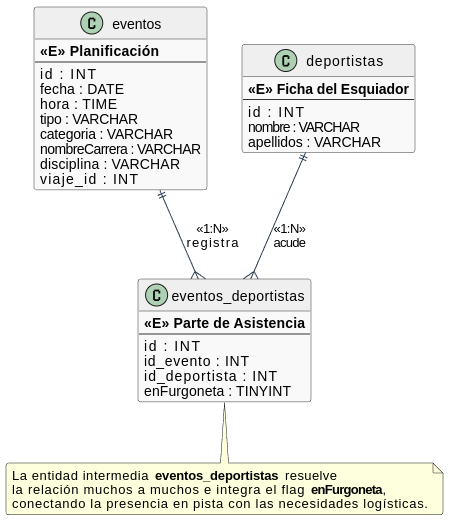
\includegraphics[width=0.65\textwidth]{diagramas/DiaagramaModeloEntrenos.drawio.png}
            \caption{Diagrama del modelo relacional de Entrenamientos y Asistencias.}
            \label{fig:relacional_eventos_asistencias}
        \end{figure}

        \subsection{Logística de Transporte}

        Este bloque del modelo de datos resuelve las necesidades operativas del club asociadas al desplazamiento de los esquiadores y el cuerpo técnico. Al centralizar la logística de transporte, el sistema optimiza la ocupación de los vehículos corporativos y furgonetas del equipo, ofreciendo además una trazabilidad completa a los tutores legales sobre el traslado seguro de los deportistas menores de edad.

        A continuación, se especifican las tablas físicas y las restricciones técnicas correspondientes a este bloque funcional del motor MySQL.
        \newpage
        \subsubsection{Tabla: transporte\_viajes}
        Representa las furgonetas, plazas habilitadas y viajes programados.

        \begin{table}[htbp]
        \centering
        \scriptsize
        \renewcommand{\arraystretch}{0.9}
        \setlength{\tabcolsep}{4pt}
        \begin{tabularx}{\textwidth}{|l|l|l|X|}
        \hline
        \rowcolor[HTML]{EFEFEF} 
        \textbf{Campo} & \textbf{Tipo de Dato} & \textbf{Clave} & \textbf{Descripción y Restricciones} \\ \hline
        \texttt{id} & INT & PK (AI) & Identificador único auto-incremental del viaje logístico. \\ \hline
        \texttt{fecha} & DATE & - & Fecha programada para la subida de los deportistas. \\ \hline
        \texttt{hora\_salida\_furgoneta} & TIME & - & Hora exacta de recogida y salida del vehículo oficial. \\ \hline
        \texttt{plazas\_totales} & INT & - & Capacidad máxima de pasajeros soportada por el vehículo. \\ \hline
        \texttt{descripcion} & VARCHAR(255) & - & Detalles de la ruta o furgoneta específica programada. \\ \hline
        \texttt{activo} & TINYINT(1) & - & Indicador booleano para habilitar o suspender las reservas. \\ \hline
        \end{tabularx}
        \caption{Especificación física de la tabla \texttt{transporte\_viajes}.}
        \label{tab:dic_transporte_viajes}
        \end{table}

        \subsubsection{Tabla: transporte\_reservas}
        Tabla intermedia encargada de consolidar y auditar de forma relacional las reservas de plazas ocupadas por los esquiadores en cada vehículo.

        \begin{table}[htbp]
        \centering
        \scriptsize
        \renewcommand{\arraystretch}{0.92}
        \setlength{\tabcolsep}{4pt}
        \begin{tabularx}{\textwidth}{|l|l|l|X|}
        \hline
        \rowcolor[HTML]{EFEFEF} 
        \textbf{Campo} & \textbf{Tipo de Dato} & \textbf{Clave} & \textbf{Descripción y Restricciones} \\ \hline
        \texttt{id} & INT & PK (AI) & Identificador correlativo único del registro de la reserva. \\ \hline
        \texttt{viaje\_id} & INT & FK & Clave foránea orientada al identificador de la tabla \texttt{transporte\_viajes}. \\ \hline
        \texttt{deportista\_id} & INT & FK & Clave foránea orientada al identificador de la tabla \texttt{deportistas}. \\ \hline
        \texttt{fecha\_reserva} & DATETIME & - & Sello temporal que registra el instante en el que se confirmó la plaza. \\ \hline
        \end{tabularx}
        \caption{Especificación física de la tabla intermedia \texttt{transporte\_reservas}.}
        \label{tab:dic_transporte_reservas}
        \end{table}

        La estructura física, las restricciones de integridad y la tipificación de los atributos de este dominio se ilustran detalladamente en el diagrama del modelo relacional de la \ref{fig:relacional_transporte_viajes}.

        \begin{figure}[htbp]
            \centering
            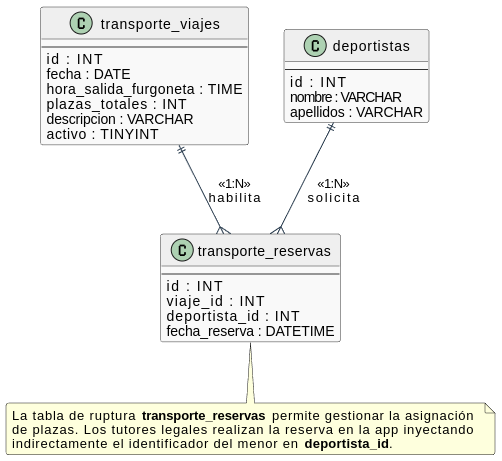
\includegraphics[width=0.65\textwidth]{diagramas/DiagramaTransporte.drawio.png}
            \caption{Modelo relacional de Transporte.}
            \label{fig:relacional_transporte_viajes}
        \end{figure}
        
        \newpage
        \subsection{Soporte y Gestión de Recursos}

        Este último bloque del modelo de datos engloba aquellas entidades diseñadas para dar soporte administrativo al proceso de incorporación a la plataforma, así como para la persistencia del archivo digital multimedia generado durante los entrenamientos en nieve. Estas tablas operan de forma transversal para garantizar la seguridad en el registro de usuarios y el análisis visual de los deportistas.

        A continuación, se especifican las tablas físicas y las restricciones técnicas correspondientes a este bloque funcional del motor MySQL.

        \subsubsection{Tabla: solicitudes\_registro}
        Actúa como tabla de tránsito para la validación previa de credenciales y datos familiares antes de su inserción definitiva en las tablas de producción del sistema.

        \begin{table}[htbp]
        \centering
        \scriptsize
        \renewcommand{\arraystretch}{0.9}
        \setlength{\tabcolsep}{4pt}
        \begin{tabularx}{\textwidth}{|l|l|l|X|}
        \hline
        \rowcolor[HTML]{EFEFEF} 
        \textbf{Campo} & \textbf{Tipo de Dato} & \textbf{Clave} & \textbf{Descripción y Restricciones} \\ \hline
        \texttt{id} & INT & PK (AI) & Identificador único auto-incremental de la solicitud. \\ \hline
        \texttt{nombre\_tutor} & VARCHAR(255) & - & Nombre de pila del padre o madre solicitante. \\ \hline
        \texttt{apellidos\_tutor} & VARCHAR(255) & - & Apellidos completos del tutor legal. \\ \hline
        \texttt{correo\_tutor} & VARCHAR(255) & - & Correo de contacto (futuro identificador de login). \\ \hline
        \texttt{nombre\_hijo} & VARCHAR(255) & - & Nombre de pila del deportista menor de edad. \\ \hline
        \texttt{apellidos\_hijo} & VARCHAR(255) & - & Apellidos completos del deportista menor. \\ \hline
        \texttt{fecha\_nacimiento\_hijo} & DATE & - & Fecha de nacimiento del corredor en inscripción. \\ \hline
        \texttt{contrasena} & VARCHAR(255) & - & Hash temporal de la clave propuesta por el usuario. \\ \hline
        \texttt{estado} & VARCHAR(50) & - & Estado de la solicitud (ej. Pendiente, Aceptada, Rechazada). \\ \hline
        \texttt{categoria} & VARCHAR(100) & - & Categoría alpina solicitada para el deportista. \\ \hline
        \texttt{fecha\_nacimiento\_tutor} & DATE & - & Fecha de nacimiento del padre o madre solicitante. \\ \hline
        \end{tabularx}
        \caption{Especificación física de la tabla \texttt{solicitudes\_registro}.}
        \label{tab:dic_solicitudes_registro}
        \end{table}
        
        \newpage
        \subsubsection{Tabla: fotos}
        Almacena la indexación y metadatos de las imágenes multimedia para la visualización técnica y el control de progreso deportivo.

        \begin{table}[htbp]
        \centering
        \scriptsize
        \renewcommand{\arraystretch}{0.9}
        \setlength{\tabcolsep}{4pt}
        \begin{tabularx}{\textwidth}{|l|l|l|X|}
        \hline
        \rowcolor[HTML]{EFEFEF} 
        \textbf{Campo} & \textbf{Tipo de Dato} & \textbf{Clave} & \textbf{Descripción y Restricciones} \\ \hline
        \texttt{id} & INT & PK (AI) & Identificador único auto-incremental del recurso multimedia. \\ \hline
        \texttt{ruta} & VARCHAR(255) & - & Dirección URL o path físico del archivo almacenado. \\ \hline
        \texttt{fecha\_creacion} & DATETIME & - & Sello temporal que registra el instante de subida del archivo. \\ \hline
        \texttt{categoria\_id} & VARCHAR(100) & - & Identificador de la categoría alpina asociada a la imagen. \\ \hline
        \end{tabularx}
        \caption{Especificación física de la tabla \texttt{fotos}.}
        \label{tab:dic_fotos}
        \end{table}

        La estructura lógica, los flujos de autoría multimedia y las relaciones de contexto de este módulo se ilustran detalladamente en el diagrama relacional de la \ref{fig:conceptual_soporte_recursos}.

        \begin{figure}[htbp]
            \centering
            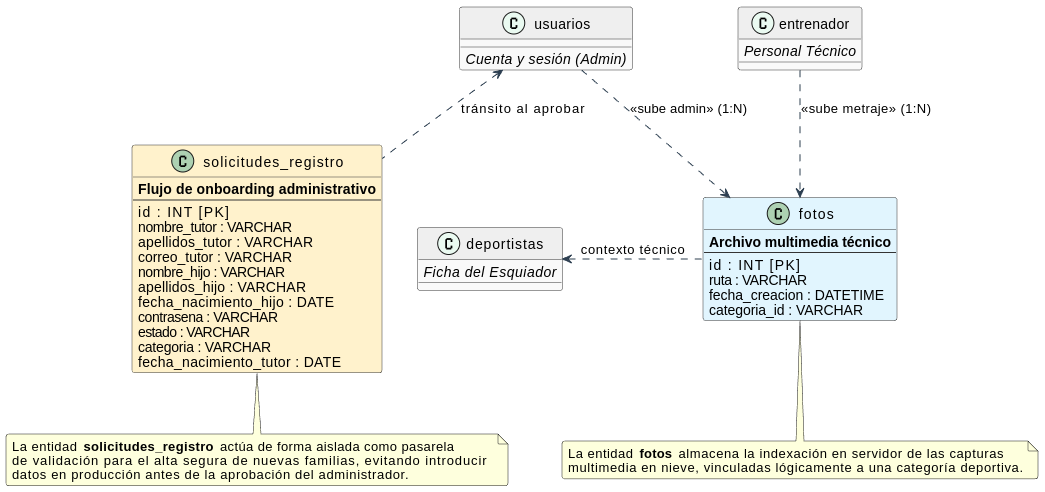
\includegraphics[width=0.8\textwidth]{diagramas/DiagramaMultimedia.drawio.png}
            \caption{Modelo de datos de Soporte y Gestión de Recursos.}
            \label{fig:conceptual_soporte_recursos}
        \end{figure}

        \newpage
        \subsection{Interfaz de usuario}
        \subsubsection{Prototipado con figma}
        Una vez definida la arquitectura conceptual y física de la base de datos, el siguiente paso en el ciclo de vida del desarrollo del software consiste en la traslación de los requisitos funcionales a un entorno puramente visual y operativo. Antes de iniciar la fase de implementación y codificación de los componentes del \textit{frontend}, se llevó a cabo un proceso iterativo de diseño de interfaces con el objetivo de modelar la experiencia de usuario (\textit{User Experience}, UX) y la consistencia visual (\textit{User Interface}, UI).

        Esta etapa de diseño previo resulta crítica en ingeniería del software por tres motivos fundamentales:
        \begin{itemize}
            \item \textbf{Mitigación de riesgos técnicos:} Permite validar los flujos de navegación lógicos del club de esquí (como el proceso de reserva indirecta de plazas o el control de asistencias) sin incurrir en costes de refactorización de código en fases avanzadas.
            \item \textbf{Garantía de usabilidad:} Asegura que tanto los tutores legales (quienes requieren interfaces directas, claras y seguras para el control de sus hijos menores) como el cuerpo técnico (que interactúa con la aplicación en entornos fríos y exteriores en las pistas de esquí) dispongan de una curva de aprendizaje mínima.
            \item \textbf{Establecimiento de una guía de estilo única:} Consolida de forma unificada la iconografía, las paletas cromáticas corporativas y las jerarquías tipográficas, sirviendo como plano técnico exacto para la posterior fase de maquetación.
        \end{itemize}

        Para la materialización de estos esquemas visuales se empleó la herramienta de prototipado industrial \textbf{Figma}. El proceso se dividió en dos fases metodológicas consecutivas: en primer lugar, se definieron los esquemas de baja fidelidad o \textit{wireframes} para estructurar la arquitectura de la información; posteriormente, se evolucionaron hacia prototipos de alta fidelidad (\textit{mockups}) que representan de forma fiel y exacta el aspecto final que adoptará la aplicación en producción.

        A continuación, se detallan los pilares visuales que gobiernan la aplicación, así como el desglose de las vistas principales agrupadas por los roles operativos del sistema.
        
        \begin{figure}[htbp]
            \centering
            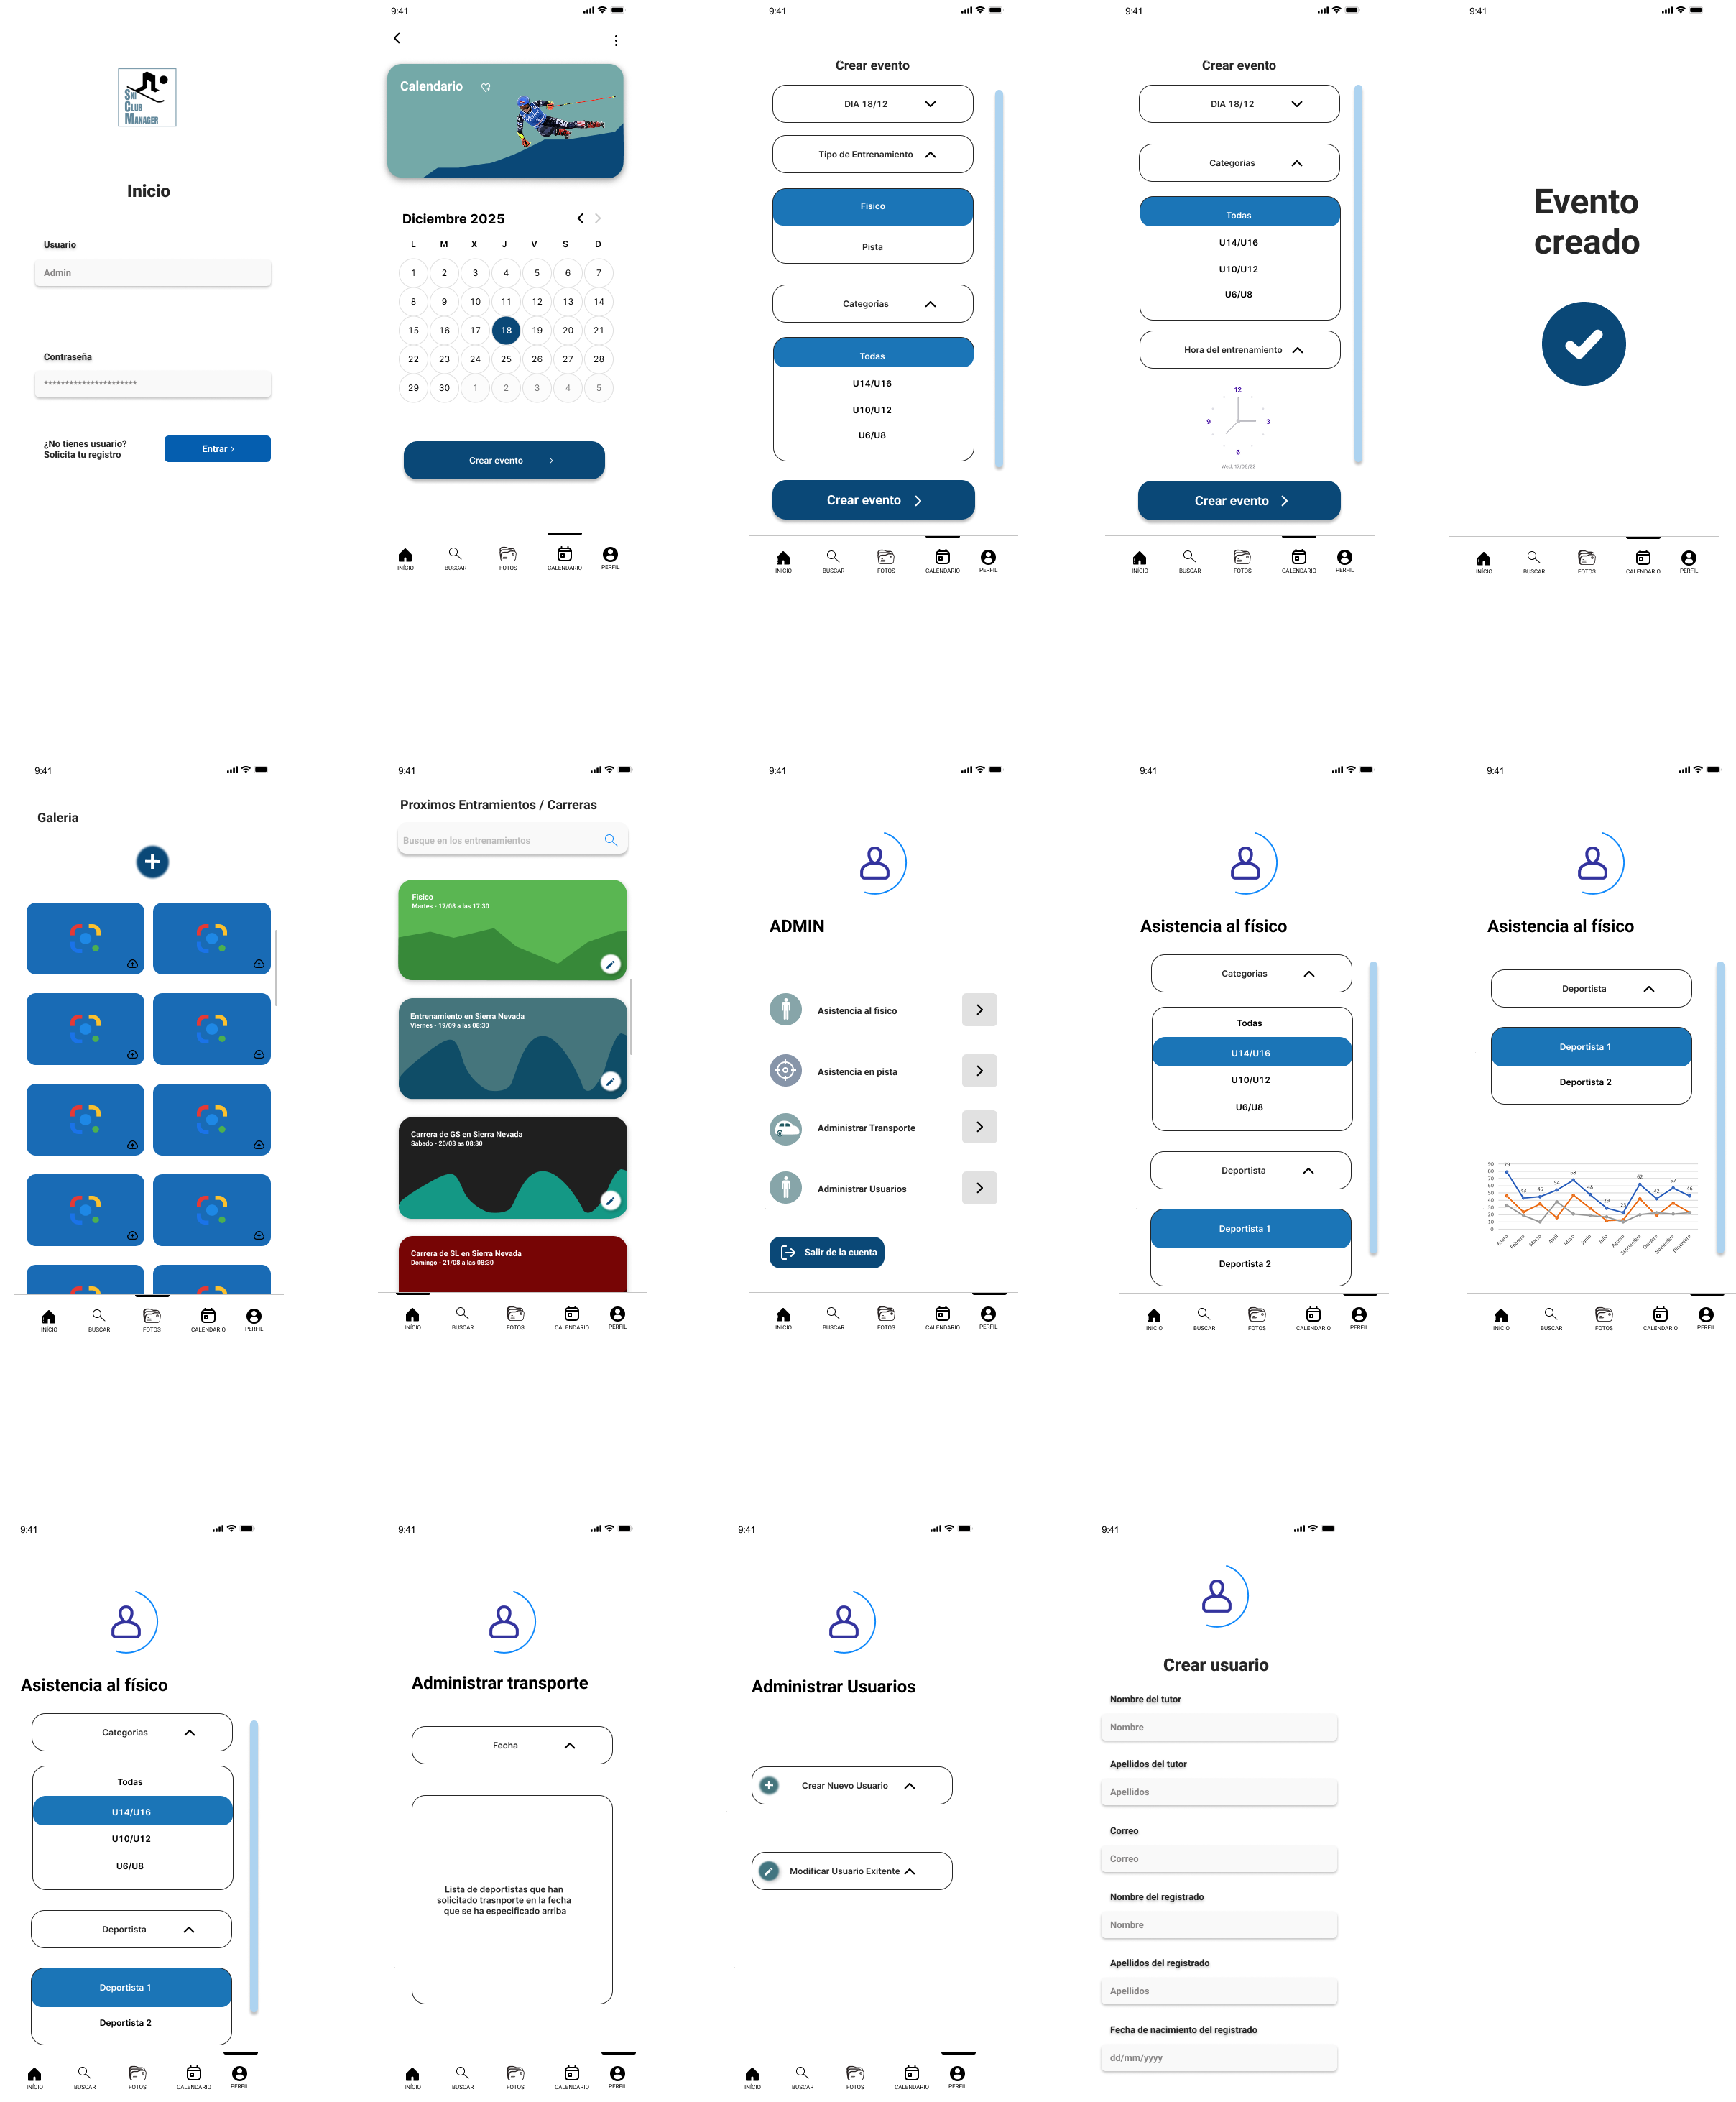
\includegraphics[width=0.8\textwidth]{imagenes/MockupAdmin.png}
            \caption{Mockup de la interfaz del administrado y del entrenador.}
            \label{fig:mockup_admin}
        \end{figure}

         \begin{figure}[htbp]
            \centering
            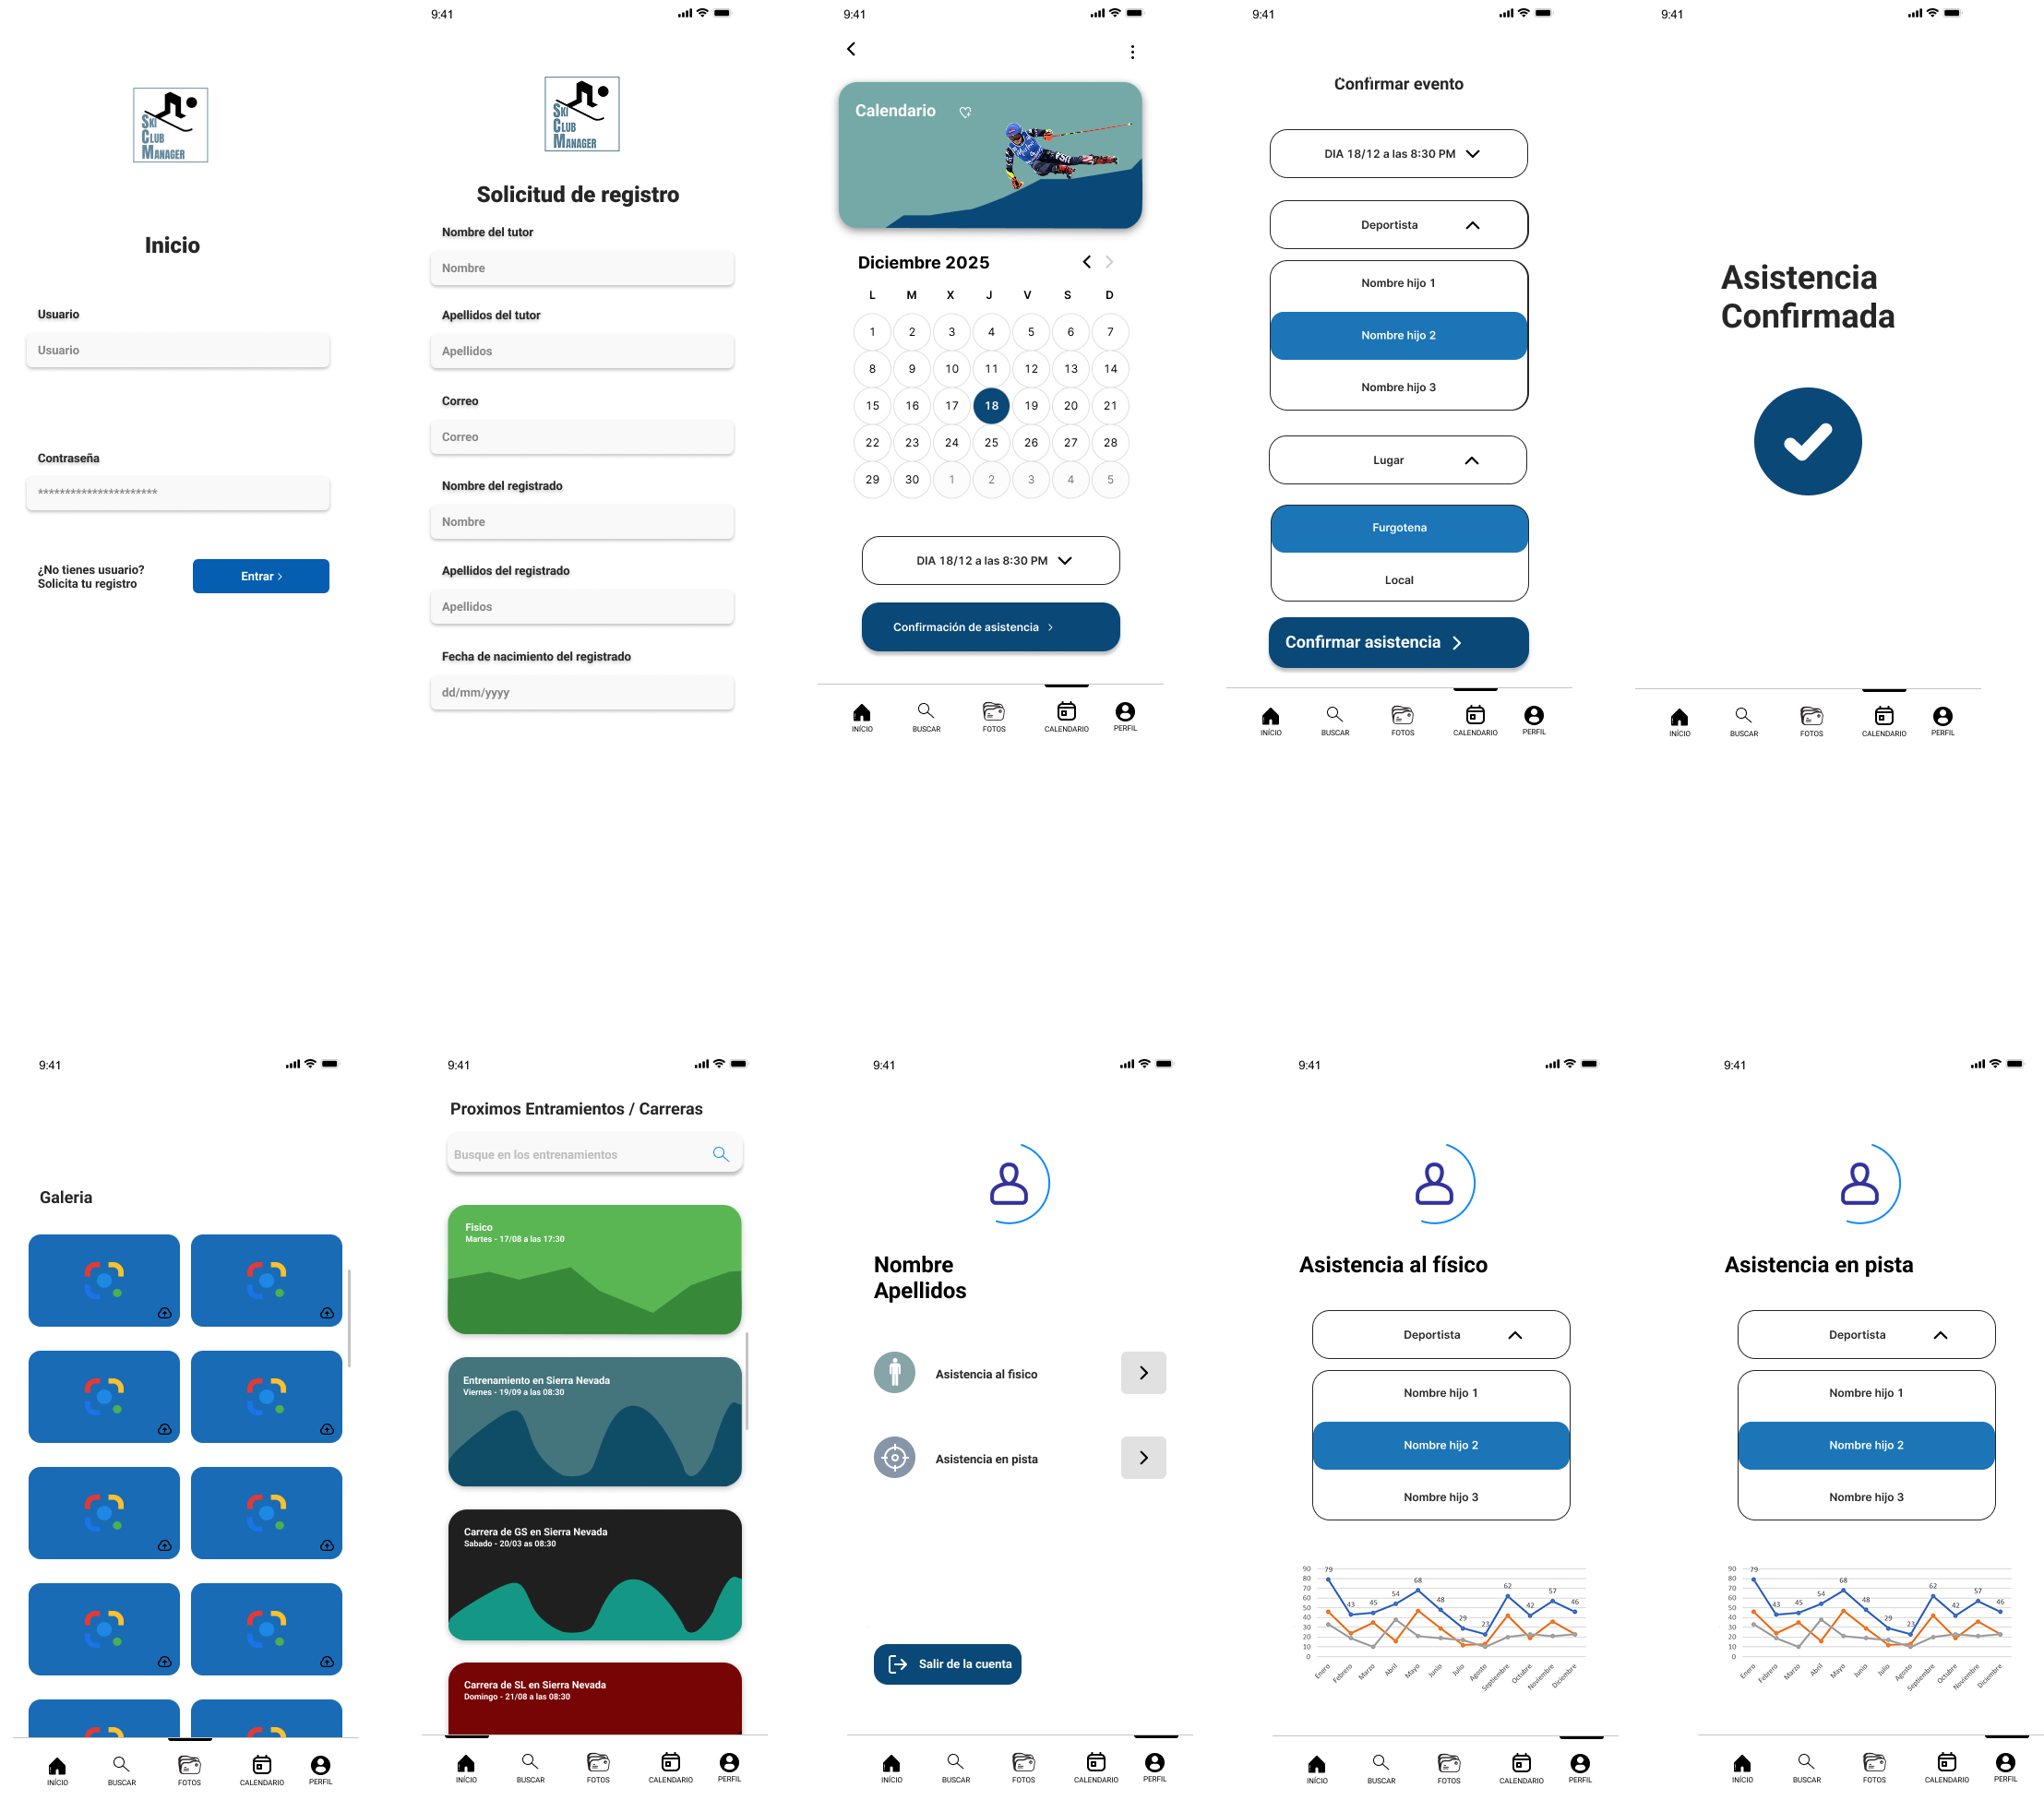
\includegraphics[width=0.8\textwidth]{imagenes/MockupPadre.png}
            \caption{Mockup de la interfaz del padre y del tutor.}
            \label{fig:mockup_padre}
        \end{figure}
        \newpage

        La fidelidad de los prototipos desarrollados en Figma y la posterior maquetación de la aplicación no son arbitrarias; responden de manera estricta a una identidad corporativa unificada. El establecimiento de este \textit{UI Kit} (Kit de Interfaz de Usuario) garantiza que cada componente visual mantenga la consistencia a lo largo de las diferentes vistas de la plataforma, reforzando la imagen institucional del club y optimizando la carga cognitiva del usuario.

        A continuación, se describen los pilares fundamentales que componen la guía de estilo del sistema.

        \subsubsection{Nombre}
        El nombre \textbf{“SkiClubManager”} fue elegido de manera estratégica para evocar la combinación exacta entre el esqui alpino de competición y la robustez de una plataforma de control administrativo moderno. Por un lado, \textbf{“SkiClub”} define de forma inequívoca el nicho y la identidad deportiva del sistema, apelando a la comunidad de corredores, entrenadores y familias que conviven en las estaciones invernales. Por otro lado, \textbf{“Manager”} alude de manera directa a la eficiencia, la automatización de procesos y el control logístico integral (asistencias, transporte y expedientes), lo cual se convierte en la metáfora perfecta del núcleo funcional del proyecto: transformar la compleja gestión manual de un club deportivo tradicional en una operativa ágil, digitalizada y centralizada en una sola herramienta.

        \subsubsection{Logo}
        El logo de la aplicación fue diseñado para capturar la esencia de “SkiClubManager”. Incluye la silueta de montañas nevadas y una flecha ascendente, lo cual simboliza tanto el entorno alpino como el progreso y la gestión deportiva del club. Se desarrolló utilizando la herramienta Figma, cuidando que los colores (tonos azules y naranja) y las formas fueran coherentes con la estética general de la aplicación, brindando una identidad visual atractiva y memorable.        \begin{figure}[htbp]
            \centering
            
\includegraphics[width=0.5\textwidth]{imagenes/logo.png}
            \caption{Diseño del logo.}
            \label{fig:diseño_logo}
        \end{figure}
        \newpage

        \subsubsection{Paleta Cromática (Colores)}
        La selección del espectro cromático responde a la identidad de los deportes de invierno y a la necesidad de ofrecer un contraste óptimo en exteriores. La paleta se compone de una base estructural de azules y un conjunto de colores semánticos destinados a la categorización visual en el módulo de calendario:

        \begin{itemize}
            \item \textbf{Color Primario y Secundario:} Tonos de azul alpino oscuro para la estructura, barras de navegación y botones principales, combinados con azul celeste para los acentos y estados activos.
            \item \textbf{Colores Semánticos del Calendario:} Para diferenciar de un vistazo el tipo de planificación en la agenda sin saturar al usuario, se utiliza un código de tres colores específicos (Rojo, Verde y Azul).
        \end{itemize}

        La definición técnica de la paleta y sus casos de uso en la interfaz se detallan en la tabla \ref{tab:paleta_colores}.

        \begin{table}[htbp]
        \centering
        \scriptsize
        \renewcommand{\arraystretch}{1.3}
        \setlength{\tabcolsep}{6pt}
        \begin{tabularx}{\textwidth}{|l|l|c|X|}
        \hline
        \rowcolor[HTML]{EFEFEF} 
        \textbf{Componente / Aplicación} & \textbf{Código HEX} & \textbf{Muestra} & \textbf{Propósito en la Interfaz (UX)} \\ \hline
        Azul Principal (Estructural) & \#2C3E50 & \colorbox[HTML]{2C3E50}{\hspace{0.4cm}} & Fondo de cabeceras, botones de acción y texto principal. \\ \hline
        Azul Celeste (Acentos) & \#3498DB & \colorbox[HTML]{3498DB}{\hspace{0.4cm}} & Elementos seleccionados, enlaces y estados activos. \\ \hline
        Verde (Calendario) & \#2ECC71 & \colorbox[HTML]{2ECC71}{\hspace{0.4cm}} & Identificación de entrenamientos de tipo físico. \\ \hline
        Rojo (Calendario) & \#E74C3C & \colorbox[HTML]{E74C3C}{\hspace{0.4cm}} & Identificación de entrenamientos técnicos en nieve. \\ \hline
        Azul Agenda (Calendario) & \#2980B9 & \colorbox[HTML]{2980B9}{\hspace{0.4cm}} & Identificación de eventos oficiales o competiciones del club. \\ \hline
        \end{tabularx}
        \caption{Especificación de la paleta de colores y lógica semántica del calendario.}
        \label{tab:paleta_colores}
        \end{table}

        \subsubsection{Componentes de la Interfaz de Usuario}

        El desarrollo del \textit{frontend} de la aplicación se ha estructurado bajo un enfoque de arquitectura basada en componentes reutilizables utilizando el framework \textbf{React Native}. Esta metodología no solo optimiza la mantenibilidad del código y reduce la redundancia, sino que garantiza un comportamiento fluido y nativo tanto en dispositivos Android como iOS, aspecto crítico para el cuerpo técnico que opera la aplicación en condiciones de baja temperatura exterior.

        A continuación, se desglosan los bloques y componentes principales que estructuran la experiencia de usuario de la plataforma:

        \subsubsection{Componentes Estructurales y de Navegación}
        Para la organización de las vistas y el flujo de pantallas se han implementado contenedores adaptativos que gestionan el ciclo de vida de la interfaz:
        \begin{itemize}
            \item \textbf{Contenedores de Pantalla (\texttt{SafeAreaView} y \texttt{ScrollView}):} Componentes encargados de garantizar que la interfaz respete las dimensiones físicas del dispositivo (evitando colisiones con \textit{notches} o barras del sistema) y permitiendo el desplazamiento vertical fluido en listados densos de deportistas o eventos.
            \item \textbf{Estructuras de Navegación (\texttt{React Navigation}):} Se combina una navegación por pestañas inferiores (\textit{Bottom Tab Navigation}) para el acceso rápido a los módulos principales (Calendario, Deportistas, Perfil) con una navegación en pila (\textit{Stack Navigation}) para flujos transaccionales profundos, tales como la apertura del expediente técnico de un corredor o la visualización de una foto en alta resolución.
        \end{itemize}

        \subsubsection{Componentes de Control de Estado y Datos}
        La sincronización de la información proveniente del \textit{backend} en Node.js y la interacción del usuario se gestionan mediante componentes de flujo de datos:
        \begin{itemize}
            \item \textbf{Proveedores de Contexto (\texttt{Context API}):} Componentes globales encargados de envolver la aplicación para inyectar el estado de la sesión, las credenciales del token JWT y el rol del usuario autenticado (Entrenador o Padre), permitiendo un renderizado condicional inmediato de la interfaz según los permisos del perfil.
            \item \textbf{Formularios Dinámicos y Entradas de Texto:} Componentes personalizados basados en \texttt{TextInput} que integran validaciones en tiempo real para procesos críticos como el inicio de sesión, la pasarela de preregistro familiar y la subida de rutas multimedia.
        \end{itemize}

        \subsubsection{Componentes Visuales Especializados y Analítica}
        Para responder a los requisitos de control de asistencia y progresión deportiva, la interfaz integra componentes enriquecidos de visualización de datos:
        \begin{itemize}
            \item \textbf{Gráficos de Progreso (\texttt{react-native-chart-kit}):} Componentes encargados de renderizar de manera interactiva las métricas de rendimiento y asistencia técnica. Utilizan gráficos de líneas y barras adaptativos que permiten filtrar la evolución del deportista por temporada o mes, facilitando a los entrenadores y padres la detección de patrones de asistencia.
            \item \textbf{Tarjetas de Expediente Familiar y Deportivo:} Presentan de forma compacta el estado de sus reservas de transporte, asistencias a pista e histórico de imágenes asociadas.
        \end{itemize}

        La organización e interconexión de estos componentes de interfaz se detalla de forma sintética en la tabla \ref{tab:componentes_ui}.

        \begin{table}[htbp]
        \centering
        \scriptsize
        \renewcommand{\arraystretch}{1.3}
        \setlength{\tabcolsep}{6pt}
        \begin{tabularx}{\textwidth}{|l|l|X|}
        \hline
        \rowcolor[HTML]{EFEFEF} 
        \textbf{Categoría} & \textbf{Componente / Librería} & \textbf{Responsabilidad en la Aplicación (React Native)} \\ \hline
        Navegación & \texttt{BottomTab / Stack} & Gestión del flujo de pantallas y menús según el rol operativo. \\ \hline
        Analítica Visual & \texttt{react-native-chart-kit} & Renderizado de curvas de progresión, estadísticas y asistencia. \\ \hline
        Gestión de Estado & \texttt{Context API} & Propagación global del estado de autenticación JWT y filtros de temporada. \\ \hline
        Interfaz Crítica & \texttt{SafeAreaView / Tarjetas} & Garantizar la legibilidad en exteriores y consistencia del diseño. \\ \hline
        \end{tabularx}
        \caption{Clasificación y responsabilidades de los componentes de la interfaz de usuario.}
        \label{tab:componentes_ui}
        \end{table}

%\frontmatter
%\tableofcontents
%\listoffigures
%\listoftables
%
%\mainmatter
%\setlength{\parskip}{5pt}

%\chapter{Introducción}
    \subsubsection{Contexto}
    El ámbito del entrenamiento deportivo de alta competición y tecnificación, específicamente en disciplinas invernales como el esquí alpino, presenta una dinámica operativa altamente compleja. A diferencia de otros deportes de interior o con instalaciones estables, la gestión de un club de esquí está condicionada por factores variables como los constantes cambios en las condiciones meteorológicas y de la nieve, y la dispersión geográfica de las estaciones de esquí.

    En este escenario, el día a día de la entidad involucra de forma directa a tres actores principales o \textit{stakeholders}: el administrador, el cuerpo técnico (entrenadores) y los tutores legales (padres). La coordinación diaria requiere gestionar flujos de información críticos en tiempo real, tales como la planificación de sesiones en pistas, los cambios de horarios de última hora, la asistencia obligatoria a los entrenamientos y el posterior análisis técnico del rendimiento.

    Tradicionalmente, las organizaciones deportivas de mediana escala han sustentado esta logística mediante metodologías analógicas o herramientas de ofimática genéricas dispersas (hojas de cálculo compartidas, anotaciones en papel y canales de mensajería instantánea informal). 
    \newpage

    \section{Motivación}
    La motivación principal de este proyecto surge de una realidad evidente en el panorama deportivo español: el esquí alpino de competición es un deporte minoritario y poco conocido a nivel nacional. Tras más de ocho años de experiencia profesional trabajando como entrenadora en este sector, se constata que esta falta de repercusión masiva provoca un vacío tecnológico absoluto. Las grandes empresas de software deportivo desarrollan plataformas pensadas exclusivamente para deportes de masas como el fútbol, el baloncesto o el \textit{running}, ignorando por completo las necesidades logísticas de los deportes de invierno. 

    Un club de esquí opera en un entorno geográfico y meteorológico extremo, donde las sesiones dependen críticamente de la nieve, el calendario es altamente variable y el soporte visual es obligatorio para la corrección técnica. Al no existir plataformas comerciales que recojan estas particularidades, los clubes se ven obligados a trabajar de forma fragmentada, utilizando hojas de cálculo genéricas o aplicaciones de mensajería informal que saturan a los entrenadores. 

    Esta experiencia acumulada a pie de pista permite identificar las ineficiencias clave que justifican el desarrollo de una solución de software a medida:
    \begin{itemize}
        \item \textbf{Inexistencia de software especializado:} Las herramientas actuales del mercado son incapaces de gestionar un calendario supeditado a la estacionalidad de las estaciones invernales ni ofrecen soluciones para las dinámicas específicas del esquí alpino, forzando al club a adaptar rudimentariamente sistemas que no han sido diseñados para su realidad.
    
        \item \textbf{Demanda de contenido visual no resuelta:} En las categorías formativas, la principal queja recurrente de las familias es la falta de acceso a los vídeos y fotos de sus hijos en pista. En este deporte, el material audiovisual no es ocio, sino una herramienta indispensable para corregir la técnica y evaluar la progresión. Al no haber un canal oficial y centralizado para compartir este material pesado, la información se dispersa y se pierde.
    
        \item \textbf{Gestión de asistencia y datos precaria:} El registro de asistencia manual o mediante plantillas aisladas impide realizar un seguimiento histórico fiable de los deportistas. La falta de una base de datos centralizada conduce a la pérdida de información crítica sobre la constancia del atleta, impidiendo que el cuerpo técnico tome decisiones basadas en datos reales a lo largo de las temporadas.
    \end{itemize}

    Frente a esta problemática, la oportunidad de diseñar e implementar un sistema de software modular constituye un reto tecnológico de ingeniería de software con un impacto directo en la productividad del club y en la optimización de la planificación deportiva.

    \section{Estado del arte}
    En esta sección se realizará un análisis exhaustivo de las soluciones tecnológicas existentes en el ámbito del software deportivo, con un enfoque específico en aquellas plataformas que, aunque no estén diseñadas para el esquí alpino, puedan ofrecer funcionalidades relevantes para la gestión de clubes deportivos. Se evaluarán herramientas de gestión de entrenamientos, aplicaciones de seguimiento de rendimiento y plataformas de comunicación entre entrenadores y familias, identificando sus fortalezas y limitaciones en relación con las necesidades específicas del esquí alpino.
    
    \begin{enumerate}
        \item \textbf{SportEasy:} Es una de las plataformas más difundidas para la gestión de equipos amateurs y clubes deportivos. Permite el control de asistencia a entrenamientos, la asignación de convocatorias y dispone de un sistema de mensajería interno. Funciona bajo un modelo de suscripción (\textit{SaaS}) y ofrece aplicaciones móviles multiplataforma.
        \item \textbf{Playoff:} Una herramienta de origen nacional muy enfocada en la administración pura de clubes (gestión de cuotas, base de datos de socios, licencias y control de accesos). Cuenta con un módulo de comunicación interna y herramientas para que los administradores centralicen los registros de los atletas.
        \item \textbf{TeamSnap:} Solución norteamericana líder en la organización de ligas y equipos deportivos. Destaca por su potente calendario indexado, su sistema de notificaciones automáticas para cambios de última hora y su panel de control para entrenadores y familias.
        \item \textbf{Sprongo:} Es la plataforma de software de análisis de vídeo de referencia en el esquí alpino de competición a nivel mundial, utilizada por equipos olímpicos y clubes internacionales. Se centra exclusivamente en el procesamiento multimedia, permitiendo la subida de vídeos en pista para realizar análisis biomecánicos, superposición de imágenes (\textit{overlay}) y corrección de virajes en cámara lenta. Sin embargo, carece por completo de un módulo administrativo relacional; no gestiona el control de asistencia diario, calendarios supeditados a la logística de la estación o perfiles diferenciados con analíticas visuales de constancia para los tutores legales.
        \item \textbf{Onesporter:} Es una plataforma digital internacional orientada específicamente al entrenamiento de deportes de invierno y esquí alpino de competición. Permite a los entrenadores planificar sesiones en nieve, registrar métricas de preparación física, gestionar el calendario de carreras y realizar un seguimiento del rendimiento del atleta. Si bien es una de las soluciones más completas para el cuerpo técnico, presenta limitaciones críticas para el escenario de un club de base: funciona bajo un modelo de suscripción individual costoso, está diseñada exclusivamente para el seguimiento del deportista de élite (dejando fuera la gestión administrativa global de un club de mediana escala), carece de un sistema relacional abierto para el control automatizado de asistencia por categorías y no ofrece un canal de comunicación directo ni analíticas visuales adaptadas para los tutores legales (padres) de categorías formativas.
    \end{enumerate}

    \hfill \break
        A continuación, se muestran pequeñas ejemplos de las 5 aplicaciones mencionadas para que puedan ser visualizadas:
    

        \begin{figure}[htbp]
            \centering
            
            % Primera fila: 2 figuras
            \begin{subfigure}{.48\textwidth}
                \centering
                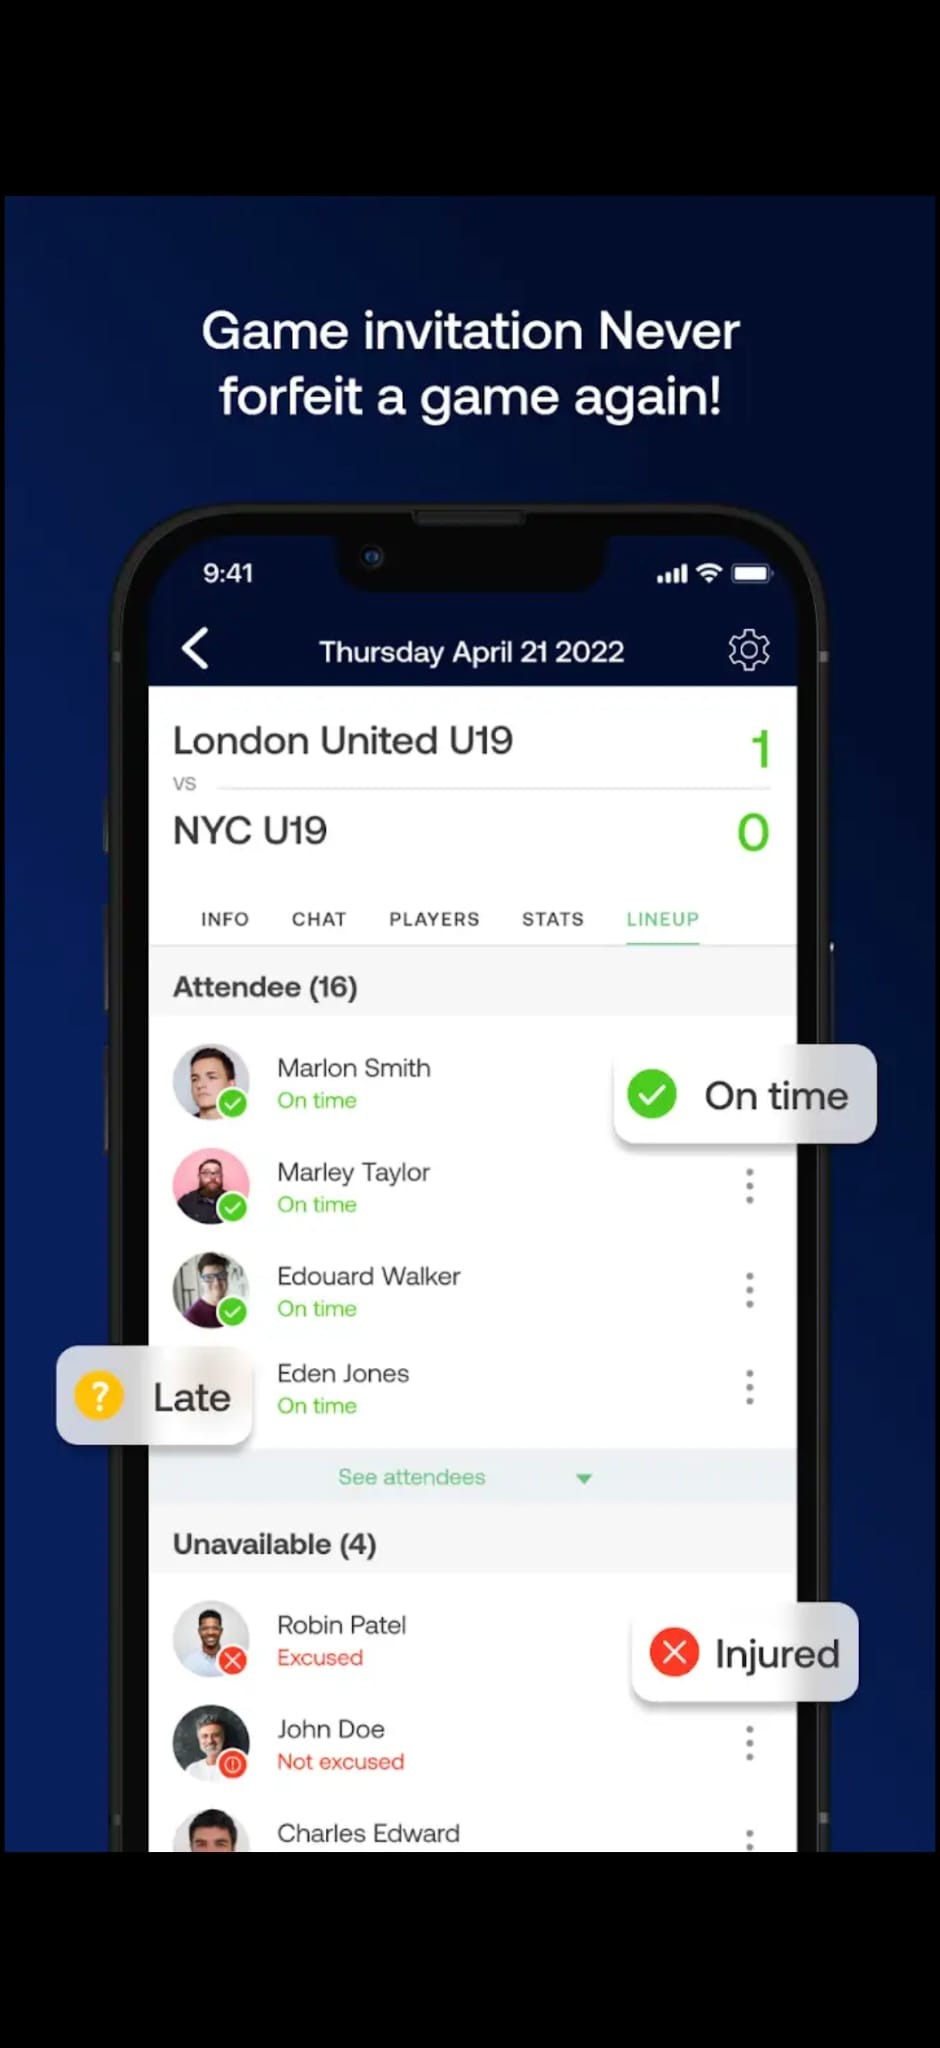
\includegraphics[width=.7\linewidth, height=1.1\linewidth]{imagenes/sportEasy.jpeg}
                \caption{SportEasy \protect\cite{SportEasy}}
                \label{fig:sporteasy_interface}            
            \end{subfigure}\hfill
            \begin{subfigure}{.48\textwidth}
                \centering
                \includegraphics[width=.7\linewidth, height=1.1\linewidth]{imagenes/Playoff.jpeg}
                \caption{Playoff \protect\cite{Playoff}}
                \label{fig:playoff_interface}            
            \end{subfigure}
            
            \vspace{0.5cm} % Espacio vertical entre la primera y segunda fila
            
            % Segunda fila: 2 figuras
            \begin{subfigure}{.48\textwidth}
                \centering
                \includegraphics[width=.7\linewidth, height=1.1\linewidth]{imagenes/TeamSnap.jpeg}
                \caption{TeamSnap \protect\cite{TeamSnap}}
                \label{fig:teamsnap_interface}            
            \end{subfigure}\hfill
            \begin{subfigure}{.48\textwidth}
                \centering
                \includegraphics[width=.7\linewidth, height=1.1\linewidth]{imagenes/Sprongo.jpeg}
                \caption{Sprongo \protect\cite{Sprongo}}
                \label{fig:sprongo_interface}            
            \end{subfigure}
            
            \vspace{0.5cm} % Espacio vertical entre la segunda y tercera fila
            
            % Tercera fila: 1 figura centrada
            \begin{subfigure}{\textwidth}
                \centering
                \includegraphics[width=.33\linewidth, height=0.52\linewidth]{imagenes/Onesporter.jpeg}
                \caption{Onesporter \protect\cite{Onesporter}}
                \label{fig:onesporter_interface}            
            \end{subfigure}
            
            \caption{Interfaces de las soluciones de software analizadas en el estudio competitivo.}
            \label{fig:analisis_competitivo_interfaces}
        \end{figure}

    \section{Objetivos}
    Dado el contexto analizado y las oportunidades de mejora detectadas, estos son los objetivos específicos del proyecto:

    \begin{itemize}
        \item \textbf{Diseñar e implementar la base de datos:} Modelar una estructura relacional en MySQL para almacenar de forma segura y organizada la información de los deportistas, entrenadores, eventos y el histórico de asistencia por temporadas.
        
        \item \textbf{Desarrollo del servicio backend:} Construir una API REST en Node.js con Express estructurada en controladores y rutas independientes para gestionar de manera eficiente todas las peticiones del sistema.
        
        \item \textbf{Garantizar la seguridad mediante roles:} Implementar un sistema de autenticación basado en JSON Web Tokens (JWT) que restrinja el acceso a las rutas del backend según el perfil del usuario (Administrador, Entrenador o Padre).
        
        \item \textbf{Crear la interfaz de usuario móvil:} Desarrollar una aplicación multiplataforma utilizando React Native y Context API que sea ligera, intuitiva y fácil de usar en las condiciones extremas a pie de pista.
        
        \item \textbf{Integrar analítica estadística visual:} Incorporar la librería \textit{react-native-chart-kit} para transformar los registros numéricos de asistencia y entrenamientos en gráficos estadísticos claros que muestren la progresión de los atletas.
        
        \item \textbf{Centralizar la gestión multimedia técnica:} Diseñar un repositorio indexado dentro de la aplicación para que los entrenadores puedan subir fotos y vídeos de los descensos, vinculándolos directamente al perfil de cada deportista para su corrección técnica.
    \end{itemize}

    Con todo ello, la gestión diaria del club de esquí y el seguimiento de los deportistas de base será no solo más eficiente y automatizado, sino también transparente y accesible para los entrenadores y las familias.
%
%\chapter{Tecnologías y Herramientas Utilizadas}
\label{cap:tecnologias_utilizadas}

El desarrollo de la plataforma \textit{SkiClubManager} se ha basado en una arquitectura desacoplada compuesta por un servicio de \textit{backend} centralizado y una aplicación móvil nativa como \textit{frontend}. La selección de la pila tecnológica (\textit{stack}) responde a criterios estrictos de rendimiento, mantenibilidad y la necesidad de ofrecer una experiencia de usuario fluida en entornos de alta montaña. A continuación, se justifican técnicamente las herramientas y entornos seleccionados.

\subsubsection{Infraestructura Backend y API REST}
Para dar soporte a la aplicación móvil y centralizar la lógica de negocio, se ha diseñado un servicio backend basado en una arquitectura cliente-servidor mediante el desarrollo de una API REST.

\subsubsection{Node.js}
Node.js es un entorno de ejecución para JavaScript construido con el motor V8 de Google \cite{NodeJS}. Su elección como núcleo del \textit{backend} se justifica por las siguientes características:
\begin{itemize}
    \item \textbf{Modelo de E/S sin bloqueo y orientado a eventos:} Utiliza un único hilo de ejecución asistido por un bucle de eventos (\textit{Event Loop}). Esto permite gestionar múltiples conexiones concurrentes de forma asíncrona sin bloquear el servidor, una cualidad crítica cuando entrenadores y familias interactúan con la aplicación simultáneamente.
    \item \textbf{Unificación del lenguaje:} El uso de JavaScript tanto en el servidor como en el cliente (\textit{frontend}) optimiza los tiempos de desarrollo, reduce la curva de aprendizaje y simplifica el mantenimiento del código fuente global.
\end{itemize}

\subsubsection{Express}
Express es un \textit{framework} minimalista y flexible creado para Node.js \cite{ExpressJS}, seleccionado para estructurar la API REST debido a su solvencia en el manejo de peticiones HTTP:
\begin{itemize}
    \item \textbf{Arquitectura basada en Middleware:} Organiza el flujo de las peticiones mediante funciones interconectadas. Esto permite auditar, transformar o validar los datos de entrada antes de que alcancen la lógica de negocio final.
    \item \textbf{Enrutamiento modular:} Permite desglosar las rutas de la API en controladores independientes, garantizando un código limpio, escalable y alineado con los principios de diseño de software modular.
\end{itemize}

\subsubsection{Motor de Persistencia: MySQL}
Como sistema de gestión de bases de datos se ha seleccionado MySQL \cite{MySQL}, un motor relacional de código abierto que garantiza el almacenamiento seguro y consistente de la información del club. Su elección se fundamenta en su capacidad para gestionar restricciones de integridad referencial mediante claves foráneas, asegurando que las asistencias, transportes y expedientes queden vinculados de forma unívoca y protegida a las fichas de los deportistas menores de edad.

\subsubsection{Desarrollo Frontend Móvil}
La capa de interacción con el usuario final requiere un entorno capaz de ofrecer portabilidad sin penalizar el rendimiento en dispositivos móviles.

\subsubsection{React Native}
React Native es un \textit{framework} de código abierto desarrollado por Meta \cite{ReactNative} que permite compilar aplicaciones móviles nativas para iOS y Android a partir de una única base de código en JavaScript y React. Los motivos técnicos de su elección incluyen:
\begin{itemize}
    \item \textbf{Renderizado Nativo:} A diferencia de las soluciones híbridas basadas en vistas web, React Native invoca directamente los componentes nativos del sistema operativo, garantizando una interfaz fluida y una respuesta inmediata a las interacciones del usuario.
    \item \textbf{Eficiencia en Entornos de Nieve:} La ligereza de la aplicación y la velocidad de respuesta de sus componentes son críticas para el cuerpo técnico en las pistas de esquí, donde las bajas temperaturas exteriores exigen flujos de trabajo rápidos y pantallas de carga mínimas.
\end{itemize}

\subsubsection{Gestión de Estado: Context API}
Para la propagación del estado global de la aplicación se ha utilizado la herramienta nativa \textit{Context API} de React. Este mecanismo permite inyectar los datos de la sesión activa, el rol del usuario autenticado (Entrenador o Padre) y los filtros temporales a lo largo de todo el árbol de componentes sin necesidad de recurrir a librerías externas complejas, facilitando el renderizado condicional inmediato de la interfaz.

\subsubsection{Autenticación: JSON Web Tokens (JWT)}
La seguridad y el aislamiento de los datos sensibles se gestionan mediante el estándar abierto RFC 7519, conocido como JSON Web Tokens \cite{RFC7519_JWT}. Tras un inicio de sesión exitoso, el servidor genera un token firmado criptográficamente que la aplicación móvil almacena de forma segura. Este token se adjunta en las cabeceras de cada petición HTTP, garantizando la autenticidad del emisor y permitiendo la validación de roles en cada \textit{endpoint} de la API REST.

\subsubsection{Visualización Analítica: React Native Chart Kit}
Para la representación gráfica del rendimiento de los corredores y los balances de asistencia en los perfiles familiares, se ha implementado la librería complementaria \textit{react-native-chart-kit} \cite{ReactNativeChartKit}. Esta herramienta se acopla directamente sobre el flujo de datos del estado global, transformando registros relacionales planos de asistencia en métricas visuales comprensibles y optimizadas para su correcta renderización en dispositivos móviles.

\subsubsection{Diseño de Interfaces: Figma}
Como entorno de prototipado industrial se ha empleado Figma. Esta herramienta basada en la nube ha permitido modelar la arquitectura de la información y evolucionar los esquemas desde \textit{wireframes} de baja fidelidad hasta los \textit{mockups} de alta fidelidad que sirven como plano técnico exacto para la maquetación visual de la aplicación móvil.
%
%\input{capitulos/03_Planificacion}
%
%\input{capitulos/04_Analisis}
%
%\input{capitulos/05_Diseno}
%
%\input{capitulos/06_Implementacion}
%
%\input{capitulos/07_Pruebas}
%
%\input{capitulos/08_Conclusiones}

%\cleardoublepage
%\phantomsection
\cleardoublepage
\printbibliography[title={Referencias Bibliográficas}]

\appendix
%\input{apendices/manual_usuario/manual_usuario}
%\input{glosario/entradas_glosario}

\chapter*{}
\thispagestyle{empty}

\end{document}